\documentclass{article}
\usepackage{geometry, graphicx, array, caption, amsmath, tikz,lscape}
\usepackage{multirow}
%\usepackage{subfigure}
\usepackage{lscape}
\DeclareMathOperator*{\argmin}{arg\,min}
\usetikzlibrary{shapes,positioning,fit,backgrounds}
\usepackage{subcaption}
\usepackage{dcolumn}
\newcolumntype{d}[1]{D{.}{.}{#1}}
\usepackage[round]{natbib}
\usepackage[colorlinks, linkcolor=black, citecolor=black, filecolor=black, urlcolor=blue]{hyperref}
%\usepackage{caption}
\usepackage[labelfont=bf,font=large]{caption}
\usepackage[hang,flushmargin]{footmisc}
\usepackage{amsfonts}
\usepackage{soul}
\usepackage{adjustbox}
\usepackage{wrapfig}
\usepackage{parskip}


\begin{document}
\setlength{\parskip}{15pt}

\title{Are Market Makers Incentivized to Provide Liquidity? Evidence from the Nasdaq}
\author{G\"{o}khan Cebiroglu \\ Nikolaus Hautsch \\ Julia Reynolds}
\date{Version: \today}
\maketitle

\begin{abstract}
\noindent Since 2002, Nasdaq has given market participants the discretion over whether to submit limit orders anonymously, or submit their orders non-anonymously along with their market participant identification number (MPID). The vast majority of non-anonymous orders are submitted by market makers, who are mandated by the exchange to submit a certain number of non-anonymous orders per day. However, while market makers are expected to fulfill this quota, the choice of when and under what circumstances to reveal their identities is still at their discretion. Therefore, in this project, we explore the determinants of MPID revelation among market makers on the Nasdaq, and the implications that these non-anonymous order submissions have for market quality.
\end{abstract}

\clearpage 

\section{Introduction}

While equity market makers were traditionally agents appointed by exchanges to maintain orderly markets and stand ready to provide liquidity, recent years have seen the rise of so-called ``endogenous liquidity providers" (ELPs), who are not appointed by exchanges but arise as liquidity providers on their own accounts.\footnote{See, e.g., \citet{bessembinder2015market,anand2016market}} The current reliance of many modern U.S. equity trading platforms on ELPs remains somewhat controversial, as exchanges have scrambled to implement programs to properly incentivize and obligate this new type of market maker to maintain orderly markets and provide liquidity.\footnote{E.g.,, the Qualified Market Maker Program on Nasdaq and the Designated Market Market Program on the NYSE.} Some questions remain as to whether exchanges have indeed been successful at this task.\footnote{For example, in a speech before the Economics Club of New York, Securities and Exchange Commission (SEC) chairman Mary L. Shapiro expressed concern ``whether the firms that effectively act as market makers during normal times should have any obligation to support the market in reasonable ways in tough times." (see ``Strengthening Our Equity Market Structure", 7 September 2010, available at \url{https://www.sec.gov/news/speech/2010/spch090710mls.htm}). In a report written in response to the May 2010 Flash Crash, a joint committee of the SEC and Commodity Futures Trading Commission (CFTC) emphasizes that ``...there remain legitimate concerns over the absence of present incentives for market participants to provide liquidity in the present market structure." (see ``Recommendations Regarding Regarding Regulatory Responses to the Market Events of May 6, 2010", 18 Februrary 2011, available at \url{http://www.cftc.gov/idc/groups/public/@aboutcftc/documents/file/jacreport_021811.pdf}).} Recent literature has focused much attention on ``market fragility": Without the presence of exchange-mandated obligations, ELPs tend to withdraw liquidity provision in unison once conditions become suboptimal and liquidity would be most needed such as in times of price uncertainty and order imbalances \citep[see, e.g.,][]{bessembinder2015market,anand2016market}. 

At the same time, there is some debate as to what the definition of a proper liquidity provider should be. According to more classical definitions of market makers, the goal of liquidity provision should simply be the ``patient" provision of limit orders, to meet demand from and help smooth out the non-synchronous arrival of ``impatient" buyers and sellers \citep[see, e.g.,][]{grossman1988liquidity}. On the other hand, more recent authors have begun to argue that, due to novel characteristics of modern markets such as high-frequency trading and dark pools, the definition of liquidity provision should be generalized. Specifically, liquidity provision should additionally be considered as the use of contrarian trading to actively correct and stabilize prices that deviate from fundamental values \citep[see, e.g.,][]{Hendershott2014405}. \citet{biais2016supplies} argue that the latter type of liquidity provision is less likely to contribute to market fragility, as such liquidity providers tend to stay in the market when price uncertainty increases. Therefore, another questions focuses on to what extent these different types of liquidity provision are incentivized without exchange-mandated obligations, and how this translates into market quality.

%%%%%%%%%%%%%%%%%%%%%%%%%%%%%%%%%%%%%%%%%%%

\noindent Another characteristic of modern equity markets that impacts the role of the market maker is that of increasing anonymity of trading. \citet{raman2014electronic} argue that an increase in market fragility is a direct result of the anonymity of modern electronic markets. In traditional floor-based markets, market makers could use reputation and long-term relationships to identify the information content of trades, and credibly discipline those who trade on private information \citep{battalio2007reputation}. However, in anonymous markets, market makers have no way of knowing the information levels of traders, which thus increases their exposure to adverse selection and incentivizes the mass withdraw of liquidity in uncertain market conditions. Furthermore, market makers may lack the incentives to reveal their own presence given a choice to trade anonymously, as non-anonymity exposes them to adverse selection in the form of pick-off risk, or serves simply to expose their own strategies and inventories.

%%%%%%%%%%%%%%%%%%%%%%%%%%%%%%%%%%%%%%%%%%%

% In an attempt to compete with anonymous ECNs, since 2002 Nasdaq has given market participants the discretion over %Given the potential benefits of anonymity in the forms of hiding trading strategies and private information, this has naturally led to a rise in anonymous trading on this electronic market. ()

%At the same time, anonymous markets also make it impossible for market makers to ``collude" with other market makers to keep spreads high and glean additional profits (). While perhaps beneficial to market quality, the inability to identify and ``sanction" market makers who undercut the prices of their fellow liquidity providers may also alter the incentives for liquidity provision in anonymous markets.

\noindent Since the introduction of SuperMontage in 2002, Nasdaq has given market participants the discretion over whether to submit limit orders anonymously, or submit their orders non-anonymously along with their market participant identification number (MPID) \citep{mizrach2006does}. At the same time, the rules governing liquidity provision on Nasdaq require that registered market makers submit a certain amount of non-anonymous, MPID-attributed quotes as part of their role as liquidity providers. Specifically, market makers are expected to stand ready and willing to buy and sell securities in which they are registered as a market maker, and to maintain continuous two-sided quotations that are attributable to the market makers by their MPID.\footnote{Nasdaq Rule 4613(a)(1): ``...the member shall be willing to buy and sell such security for its own account on a continuous basis and shall enter and maintain a two-sided quotation (`Principal Quote'), which is attributed to the market maker by a special maker participant identifier (`MPID')...". See \url{http://Nasdaq.cchwallstreet.com/Nasdaq/pdf/new_listing_rules.pdf}.} Nasdaq's Qualified Market Maker (QMM) program broadens these obligations somewhat, stipulating that a QMM must, on a daily basis, post displayed quotes during at least 25\% of trading hours in at least 1,000 securities.\footnote{See \url{http://Nasdaq.cchwallstreet.com/Nasdaq/main/Nasdaq-equityrules/chp_1_1/chp_1_1_4/chp_1_1_4_6/chp_1_1_4_6_5/chp_1_1_4_6_5_4/default.asp}.} In return, market makers receive additional rebates on liquidity provision, along with other privileges. However, given their fulfillment of this quota of MPID-attributed orders, the choice of when and under what circumstances to reveal their presence is still at the discretion of the individual market maker. This has put modern market makers at a crossroads in terms of fulfilling their obligations as market makers, against avoiding adverse selection and exposure in highly anonymous markets.

\noindent Therefore, this paper explores the nature of the market maker incentive program's required exposure of market maker MPIDs, and to what extent this rule may in turn constrain market makers more than incentivizing them to adequately supply liquidity. Accordingly, we explores the determinants of non-anonymous intervention by market makers on the Nasdaq, and the implications that this may have for market quality. Specifically, this paper asks: Are MPID-attributed orders submitted by market makers in line with their obligations to provide liquidity? To what extent to they respond to market conditions in which they must intervene as ``reliable counterparties", and to what extent do they act as ``contrarian traders", according to the two definitions of liquidity provision? Secondly, how does the market react to non-anonymous orders posted by market makers? In order to address these questions, we use a unique dataset that reconstructs the limit order book for several Nasdaq-traded stocks. Our data contains information on whether or not a limit order is submitted anonymously, and, given non-anonymity, the market participant identifier number (MPID) of the submitter. This allows us to identify the non-anonymous orders submitted by market makers. In answering these questions, we aim to contribute insights into whether liquidity provision incentive schemes put into place by modern exchanges indeed properly incentivize market makers to maintain orderly markets and provide liquidity when it is needed.

\noindent Our paper is most closely related to that of \citet{comerton2011traders}, which examines the determinants and impact of anonymous trading on the Toronto Stock Exchange, using trading book data from 1 May to 31 July 2004. These authors find that traders use anonymity when submitting informed orders, and that anonymity can reduce the executions costs of orders that are large and aggressive. However, it should be noted that the properties of their dataset hint that TSX at this period of time had a very different trading landscape than that of the present study. While 2.86\% of orders in our sample are submitted non-anonymously, in the dataset of \citet{comerton2011traders} about 94\% are submitted non-anonymously. Furthermore, TSX stocks each have a designated market maker firm who is compensated directly by the issuer for maintaining an orderly market in that stock; such contracts are currently illegal in the U.S. under FINRA Rule 5250.\footnote{See FINRA Rule 5250, Payments for Market Making: ``No member or person associated with a member shall accept any payment or other consideration, directly or indirectly, from an issuer of a security, or any affiliate or promoter thereof, for publishing a quotation, acting as market maker in a security, or submitting an application in connection therewith." Available at \url{http://finra.complinet.com/en/display/display_main.html?rbid=2403&element_id=8626}.} In addition, our paper is related to two working papers. Both \citet{benhami2006liquidity} and \citet{karam2012} examine the value of the choice of (non-) anonymity on Nasdaq traders; however, both papers use datasets that pre-date the implementation Regulation National Market System (Reg NMS), after which most trading shifted onto ECNs that more easily facilitate anonymous trading.

\noindent Our main results can be summarized as follows. In terms of the determinants of market maker MPID attribution, results from a panel regression of MPID-attributed submission intensities on lagged market conditions are consistent with the hypothesis that the market makers submit MPID-attributed orders in their capacity to provide liquidity, but only as far as they respond to market conditions in which the supply of limit orders is low. A one-standard deviation decrease in submission volumes leads to a relative increase in MPID-attributed submissions by market makers of 3-6\%, and a one-standard deviation decrease in depth increases MPID-attributed submissions by about 1-3\%. MPID-attributed order submissions by market makers are also higher following intervals of high volatility and high relative bid-ask spreads, reflecting a response to illiquid conditions on the limit order book. However, market makers are not shown to respond with MPID-attributed orders to intervals of high pricing errors (as measures by the \citet{hasbrouck1993assessing} measure), nor are they shown to submit orders that would act against movements in prices. Therefore, Nasdaq's incentive program seems to encourage interventions by market makers in the sense of a more classical definition of liquidity provision, but does not necessarily encourage them to intervene to correct and stabilize prices.

As for the market's reaction to MPID-attributed submissions by market makers, we use a instrumental variable panel regression of market quality measures on lagged measures of MPID-attributed order submission intensities, in which MPID-attributed submission intensities are instrumented using the average MPID-attributed submission intensities in other sample stocks. The results indeed show that MPID-attributed orders by market makers succeeds at increasing the number of executions. A one-standard-deviation increase in the intensity of MPID-attributed submissions increases execution volumes by 14-40\%. However, this increased rate of market participation does not seem to translate into an improvement in market quality. There is little evidence that MPID-attributed orders are followed by lower relative bid-ask spreads or volatility, and are furthermore shown to potentially increase the presence of pricing errors by 9-36\%.

Taken together, these results show that, while liquidity provision incentive programs on Nasdaq indeed encourage market makers to submit patient limit orders to meet liquidity demand, there are little incentives for them to respond to correct de-stabilized prices. In fact, the requirement that they reveal their MPID, thereby exposing themselves to adverse selection, may strongly reduce their incentives to intervene in response to pricing errors. Since little improvement in market quality is found absent this incentive, the ``contrarian trader" role of liquidity provision may be crucial in transferring the incentives to provide liquidity into real benefits for modern markets.

\noindent The remainder of this paper is organized as follows. Section~\ref{hypothesis} describes the economic foundations to our paper and lays out our hypotheses regarding the determinants of and market reactions to non-anonymous market maker intervention. Details on our unique dataset, along with descriptions of the MPID data and our measure of MPID submission intensity, are provided Section~\ref{data}. Section~\ref{determinants} describes the methodology and empirical results for our question on the determinants of market maker intervention, while Section~\ref{reactions} does the same addressing our question regarding market reactions to market makers' non-anonymous interventions. Finally, Section~\ref{conclusion} concludes.

\section{Economic Foundations}\label{hypothesis}

The first aim of our paper is to address the question: Do market makers submit non-anonymous orders according to their obligations to provide liquidity? In order to examine this question, it is of course first necessary to clarify what the purpose and function of a market maker as a provider of liquidity should be.

A more classic definition of liquidity provision tend to focus on liquidity providers as ``patient" traders, who submit limit orders to meet liquidity demand from market-order-submitting ``impatient" traders. The idea centers around the submission of limit orders, which lets liquidity providers smooth out the different arrival times of impatient buyers and sellers. In his seminal paper, \citet{demsetz1968cost} identifies the non-synchronous arrival of buyers and sellers into a market as one of the key frictions in financial markets. However, he proposes that this problem can be alleviated by market makers who bridge the gaps between these non-synchronous arrivals. In subsequent papers, \citet{garbade1979structural} and \citet{grossman1988liquidity} show that market makers help to mitigate order imbalances and lower execution risk for other market participants. According to this ``reliable-counterparty" definition, the main role of market makers should be to serve as reliable counterparties to traders when no others are available.

Guided by this intuition, if liquidity providers are indeed properly incentivized and/or obligated to act as market makers according to this definition, then submitted quotes that are attributed to a market maker MPID should reflect this role. We would expect to see a higher rate of MPID-attributed quotes when limits orders are insufficient to meet liquidity demand: i.e., when available depth is relatively low, order submissions are relatively low, and order executions are relatively high.\footnote{In an alternative hypothesis, market makers may also submit limit orders when executions are low, if they expect that their orders will attract executions by ``reactive traders" in the spirit of \citet{harris1997order}.} We might also see a higher rate of MPID-attributed quotes when depth on the books is low, as this represents a low supply of limit orders. %Furthermore, market participation has been shown to drop during market downturns \citep[see, e.g.,][]{naes2011stock}; therefore, we might also expect to see a higher rate of MPID-attributed quotes following large, negative movements in prices.

On the other hand, with the rise of modern electronic market structures and changing incentives for traders, some have argued that the definition of what it means to supply liquidity requires a further update. According this more ``modern" definition, liquidity providers should be seen as ``contrarian" traders who prevent large pricing fluctuations by trading against error-driven price movements, and in this sense can supply liquidity even through aggressive or marketable orders.\footnote{Note that our dataset does not allow for the identification of MPID-attributed market orders. Therefore, price aggressiveness (the distance of a limit order to the midquote) serves as a proxy for the ``marketability" of an MPID-attributed order.}  Using a state-space model, \citet{Hendershott2014405} show that specialists on the NYSE respond to price pressures and seek to revert pricing errors by trading against them, thus showing the tendency of liquidity providers to trade against transitory price movements. Other recent papers to use this concept of liquidity provision as the provision of contra-side trades can be found, for example, in the literature on liquidity provision by institutional investors \citep[][]{franzoni2013constrains}, liquidity provision in dark pools \citep[][]{boni2013dark}, and liquidity provision by proprietary traders \citep[][]{biais2016supplies}. This ``contrarian-trader" definition tells us that the role of the market maker should be to stabilize markets in the face of price uncertainty.

In this case, we would also expect to see a higher rate of MPID-attributed quotes when uncertainty in prices is high. Uncertainty in this case refers to an occasion in which asset prices deviate significantly from fundamental underlying values. This is typically measured using asset volatility \citep[see, e.g.,][]{chung2014uncertainty}. Furthermore, higher uncertainty is also associated with higher illiquidity as measured by the relative bid-ask spread, as (1) illiquidity prevents information from being quickly incorporated into prices \citep[see, e.g.,][]{chordia2008liquidity}, and (2) uncertainty about prices exposes traders to higher adverse selection as in the classic ``lemons problem" of \citet{akerlof1995market}, and higher adverse selection in turn leads to higher spreads \citep[see, e.g.,][]{kyle1985continuous,huang1997components}. Following this definition of liquidity provision as ``contrarian" trading, we might also expect to see higher rate of MPID-attributed errors following significant directional changes in prices.

Note that these roles are not mutually exclusive, and difficult to entangle empirically. As an example, if market makers are shown to increase buy-side MPID-attributed orders following periods of low buy-side depth, this could be because they are responding to a low supply of limit orders, and/or because they are responding to price pressures by sell market orders that are ``eating up" depth on the buy side side of the book. A reaction to low submission volume could stem from market makers' incentives to re-supply limit orders, or stem from a reaction to the substitution of market for limit orders as market participants react quickly to changing prices. Market makers may react to high volatility or relative bid-ask spreads in order to stabilize markets, or they may simply be reacting to a thin limit order book, in which spreads are wide and depth is not sufficient to absorb market orders without frequent changes in the price. However, some variables may allow us to tease out a distinction between these two different roles. If market makers submit MPID-attributed orders according to this first definition of liquidity provision, we might expect to see that MPID-attributed orders are less aggressive on average. This does not necessarily fit the role of liquidity provision according to the second definition. In the same vein, if market makers use MPID-attributed according to this second definition, then we might expect to see a higher MPID submission following large price changes, or following an increase in pricing ``noise" (as measured using, e.g., the \citet{hasbrouck1993assessing} definition of pricing errors). This brings us to the following hypotheses:

%Lastly, as large, aggressive orders are typically associated with the highest price impact and risk of informed trading \citep[see, e.g., ][]{easley1987price,JOFI:JOFI5192,kaniel2006so}, market makers may avoid the use of such orders to further avoid any destabilizing price effects from a new submission. Therefore, market makers may be more likely to submit orders that are smaller and less aggressive.

%\noindent\fbox{
\parbox{\textwidth}{
\noindent \textbf{Hypothesis 1}: If the MPID-attributed orders are submitted by market makers in their capacity as liquidity providers, then we should see an increase in MPID submission in response to: (a) lower submission volume and higher execution volume; (b) lower depth; (c) higher volatility; and (d) higher bid-ask spreads. \\
\noindent \textbf{Hypothesis 1a}: If MPID-attributed orders are submitted by market makers in the capacity as ``contrarian traders", then we should see an increase in MPID submission in response to: (e) large prices changes; and (f) an increase in pricing errors. \\
\noindent \textbf{Hypothesis 1b}:If MPID-attributed orders are submitted by market makers in the capacity to serve as ``reliable counterparties", then MPID-attributed orders should be (g) less aggressive on average.
}
%}

The second aim of our paper is to answer the question: How does the market react to non-anonymous orders posted by market makers? By submitting an MPID-attributed order, a market maker essentially reveals two important signals, to which the market can react. The first signal can be tied to the nature of the order as non-anonymous. Numerous papers on trader anonymity have shown that informed traders prefer to submit their orders anonymously, to prevent other traders from discovering their information or trading strategies \citep[see, e.g.,][]{grammig2001knowing,barclay2003competition,comerton2011traders}. As the submission of an non-anonymous orders by market makers is mandated by Nasdaq, this potentially exposes market makers to increased adverse selection, depending on the types of traders that are attracted to trade against their orders. Following \citet{harris1997order}, order exposure may on the one hand encourage market participation from so-called defensive, ``reactive" traders,  who wait to be presented with valuable trading opportunities rather than initiating a trade and potentially exposing themselves to informed trades. Increased market participation from this type of trader, whose orders may provide as well as take liquidity, may improve liquidity conditions on and thus the overall market quality of the limit order book. On the other hand, if MPID-attributed orders are seen by the market as containing some amount of information (e.g., information about trading strategies or inventories), order exposure could also potentially encourage reactions by so-called ``parasitic" traders, who trade in order to take advantage of the information they glean from exposed orders. \citet{harris1997order} argues that these types of traders do not improve or can even deteriorate market quality, as these orders take, rather than supply, liquidity, and furthermore make no contributions to price efficiency. In either case, we would expect to see market participation rates rise following MPID-attributed orders; however, whether the increase in market participation leads to an improvement in market quality may depend on the types of traders that are attracted.

The second signal stems from the fact that, since the MPID reveals the full identity of the submitter, MPID attribution also reveals that the order is submitted by a market maker. Given regulatory concern over low investor confidence in liquidity providers since the 2010 Flash Crash, the revealed presence of a reliable liquidity provider may serve to boost investor confidence and stabilize uncertain markets \citep[see, e.g.,][]{watanabe2015,anand2016market}. As a result, we might see lower volatility in response to an MPID-attributed order. Particularly if the market can observe market makers acting to smooth out pricing errors, MPID-attributed order may be viewed as ``anchoring" the price on the side of the book (buy or sell) to which it is submitted. Therefore, we might also see a drop in pricing errors.  This leads to the following hypotheses:

%\noindent\fbox{
\parbox{\textwidth}{
\noindent \textbf{Hypothesis 2}: If the MPID-attributed orders are submitted by market markers in their capacity as liquidity providers, then in response to higher rates of MPID submission we should see: (a) higher execution and submission volume. \\
    \textbf{Hypothesis 2a}: If the MPID-attributed orders orders encourage market participation by reactive (v.s. parasitic traders), then in response to higher rates of MPID submission we should see: (b) higher depth; (c) lower bid-ask spreads; and (d) lower volatility. \\
\noindent \textbf{Hypothesis 2b}: If MPID-attributed orders are submitted by market makers in the capacity as ``contrarian traders", then in response to higher rates of MPID submission we should see a (e) decrease in pricing errors.
}

%}

%\noindent On the other hand, the literature shows a range of alternative motivations that can drive the determinants of and reactions to market maker order submissions, particularly within the context of market transparency. \citet{simaan2003market} argue that non-anonymity allows market makers to form a regime that enforces an implicit collusion to keep spreads wide, in which defecting market makers can be identified and punished. Furthermore, market makers are occasionally treated in the literature as informed traders, as they can receive information from either their associated clients \citep{saporta1997inter,naik1999trade} or make inferences from their knowledge of order flow, particularly in the the case of high-frequency market makers \citep{vayanos2001strategic,van2016high,malinova2016modern}.\footnote{Other prominent examples include \citet{boulatov2013hidden} and \citet{kaniel2006so}, who examine the endogenous choice of informed traders to submit limit or market orders. \citet{kaniel2006so} shows that informed traders with long-lived information tend to prefer limit orders, and that price impacts following limit orders tend to be higher.} As argued by \citet{karam2012}, the fact that market makers are constrained to provide MPID-attributed quotes increases the likelihood that even their non-anonymous quotes will contain some degree of their information. Furthermore, \citet{reiss2005anonymity} show that, even when an anonymous market is available, market makers prefer to submit their informed trades non-anonymously, in order to avoid a downward spiral in which too many anonymous informed trades increase adverse selection and crowd out liquidity. Lastly, market makers may also use their MPID-attributed orders in attempts to ``bluff" the market. \citet{foucault2013market} and \citet{karam2012} argue that, when market makers are aware that their orders will signal information, they will post non-anonymous quotes at the best bid or ask when spreads are large.

\noindent Overall, if market makers are indeed properly incentivized and/or obligated to use their MPID-attributed orders to encourage market participation and to stabilize markets, then these incentives should be reflected in the MPID's strategic choice of when to submit a non-anonymous order, as well as reflected in the market's reaction to an MPID-attributed order. Deviations from Hypotheses 1 and 2 should reflect an alternative motivation for the market maker's submission of MPID-attributed orders, and thus a deviation from the principal goals of exchange-mandated market maker incentive programs.

\section{Data}\label{data}

Data is obtained from LOBSTER\footnote{Limit Order Book System -- The Efficient Reconstructor; see \url{https://lobsterdata.com/}.} Academic Data, an online data tool that reconstructs the limit order book for the universe of Nasdaq stocks using the Nasdaq TotalView-ITCH direct data feed. The dataset includes order book data on prevailing bid and ask quotes and depths at up to 200 price levels, as well as message files that contain updates to the limit order book. This includes information on the type of event (submissions, partial or total cancellations, and executions of visible or hidden orders), the number of shares, price, direction (buy or sell), and time stamp (to the nanosecond) of the order that the event concerns, as well as a unique order reference number that allows us to track the submission and eventual execution or cancellation of the order. In addition, our data sample uniquely contains information on the Market Participant Identification Number (MPID). This will be described in more detail in Section~\ref{subsec:MMID}.

\noindent The main sample in this analysis is composed of eight Nasdaq-listed firms, mostly in the high-tech industry. These firms include: Apple, Inc. (AAPL); Cisco Systems, Inc. (CSCO); eBay, Inc. (EBAY); Facebook, Inc. (FB); Google, Inc. (GOOG); Intel Corporation (INTC); Microsoft Corporation (MSFT), and Yahoo! Inc. (YHOO). The sample time period includes 14 trading days in November 2013, from 4 November to 22 November 2013.\footnote{It was necessary to exclude 11 November 2013 due to corrupt data files.} Summary statistics for the stock prices, returns, and order flow for these firms is presented in Table~\ref{tab:desstats}. From the summary statistics we can see, first, a wide dispersion in share prices between the sample stocks. The two highest-priced stocks (GOOG, at \$1025.43; and AAPL, at \$521.25) are particularly distinct from the other stocks, as they have stocks prices that are an order of magnitude higher than the next highest-priced stock (EBAY, at \$51.94). Furthermore, these stocks also differ widely in terms of order flow. While GOOG has just over 5,000 average daily trades, FB has nearly eleven times as mainly, at nearly 55,000 average daily trades. Lastly, five out of the eight stocks experience, on average, negative daily returns, implying that this time period may be in one in which the market is in particular need of stable liquidity provision by market makers. Also reported for each firms are the percentages of total order submissions that are attributed to an MPID. MPID-attribution rates range from a low of 1.61\% for MSFT, to a high of $6.80\%$ for FB.

\begin{table}[h!]
\caption{Sample Stocks Descriptive Statistics} \label{tab:desstats}
\begin{center}
\resizebox{\textwidth}{!}{%
\begin{tabular}{p{2.5in}>{\centering\arraybackslash}m{1in}>{\centering\arraybackslash}m{1in}>{\centering\arraybackslash}m{1in}>{\centering\arraybackslash}m{1in}>{\centering\arraybackslash}m{1in}} \hline
  \hline
\multicolumn{6}{c}{}\\
     & \textbf{Mean} & \textbf{Median} & \textbf{Std. Dev.} & \textbf{Min.} & \textbf{Max.} \\
\textbf{AAPL} \\
Average Stock Price (USD)            & 521.25     & 520.43     & 3.66       & 512.38    & 529.27        \\
Daily Return (bp)                    & -0.10      & -0.21      & 1.00       & -1.61     & 1.57          \\
Number of Daily Orders               & 138,681    & 137,088    & 23,008     & 96,796    & 186,736       \\
Number of Daily Trades               & 16,368     & 15,555     & 2,500      & 13,614    & 21,515        \\
\% MPID & 1.96\% \\
%$\Delta t$ & $1.58$ & $0.72$ & $2.26$ & $0.00$ & $28.67$ \\
\textbf{CSCO} \\
Average Stock Price (USD)            & 22.11       & 21.47       & 1.03       & 20.77      & 24.00        \\
Intradaily Return Volatility (bp)    & 0.0022      & 0.0015      & 0.0028     & 0.0013     & 0.0121       \\
Daily Return (bp)                    & -0.34       & 0.70        & 3.31       & -10.84     & 2.13         \\
Number of Daily Orders               & 249,443     & 244,267     & 90,655     & 152,238    & 536,612      \\
Number of Daily Trades               & 22,544      & 19,668      & 13,670     & 12,247     & 67,736       \\
\% MPID & 2.14\% \\
%$\Delta t$ & $1.40$ & $0.35$ & $2.11$ & $0.00$ & $22.34$ \\
\textbf{EBAY} \\
Average Stock Price (USD)            & 51.94      & 52.15      & 1.07       & 49.87      & 53.85        \\
Daily Return (bp)                    & -0.15      & -0.30      & 1.68       & -3.34      & 4.31         \\
Number of Daily Orders               & 310,645    & 286,657    & 113,001    & 164,888    & 597,135      \\
Number of Daily Trades               & 20,620     & 17,564     & 7,797      & 13,560     & 40,018       \\
\% MPID & 3.84\% \\
%$\Delta t$ & $1.40$ & $0.54$ & $1.97$ & $0.00$ & $18.90$ \\
\textbf{FB} \\
Average Stock Price (USD)            & 47.89       & 47.89       & 1.13       & 45.73      & 50.45        \\
Daily Return (bp)                    & -0.29       & 0.04        & 2.84       & -6.49      & 4.51         \\
Number of Daily Orders               & 638,182     & 649,744     & 162,879    & 369,426    & 852,392      \\
Number of Daily Trades               & 54,356      & 59,540      & 13,418     & 32,768     & 78,343       \\
\% MPID & 6.80\% \\
%$\Delta t$ & $0.29$ & $0.02$ & $0.72$ & $0.00$ & $17.54$ \\
\textbf{GOOG} \\
Average Stock Price (USD)            & 1025.43   & 1025.80   & 9.58      & 1005.00   & 1048.80      \\
Daily Return (bp)                    & 0.05      & -0.15     & 0.88      & -1.48     & 2.05         \\
Number of Daily Orders               & 75,042    & 76,744    & 19,323    & 49,241    & 114,180      \\
Number of Daily Trades               & 5,187     & 4,710     & 1,395     & 3,531     & 7,935        \\
\% MPID & 1.81\% \\
%$\Delta t$ & $2.52$ & $0.44$ & $5.01$ & $0.00$ & $98.35$ \\
\textbf{INTC} \\
Average Stock Price (USD)            & 24.36       & 24.34      & 0.33       & 23.77      & 25.28        \\
Daily Return (bp)                    & -0.11       & 0.29       & 1.88       & -5.35      & 2.69         \\
Number of Daily Orders               & 190,832     & 172,346    & 49,940     & 138,646    & 326,237      \\
Number of Daily Trades               & 14,174      & 12,548     & 5,644      & 9,398      & 31,298       \\
\% MPID & 1.89\% \\
%$\Delta t$ & $1.47$ & $0.30$ & $2.33$ & $0.00$ & $23.48$ \\
\textbf{MSFT} \\
Average Stock Price (USD)            & 37.34       & 37.45       & 0.55       & 35.55      & 38.22         \\
Daily Return (bp)                    & 0.35        & 0.43        & 1.71       & -1.77      & 4.18          \\
Number of Daily Orders               & 444,870     & 426,755     & 105,221    & 269,153    & 640,988       \\
Number of Daily Trades               & 29,026      & 27,207      & 10,764     & 16,448     & 57,101        \\
\% MPID & 1.61\% \\
%$\Delta t$ & $0.84$ & $0.08$ & $1.60$ & $0.00$ & $21.85$ \\
\textbf{YHOO} \\
Average Stock Price (USD)            & 34.56      & 34.85      & 1.32       & 32.07      & 36.66        \\
Daily Return (bp)                    & 0.75       & 0.52       & 1.94       & -2.40      & 3.15         \\
Number of Daily Orders               & 378,733    & 358,077    & 124,213    & 208,150    & 552,838      \\
Number of Daily Trades               & 21,726     & 22,149     & 5,121      & 15,623     & 34,732       \\
\% MPID & 2.85\% \\
\\ \hline
%$\Delta t$ & $1.07$ & $0.06$ & $2.04$ & $0.00$ & $26.31$
  \hline
\end{tabular}}
\end{center}
\noindent \footnotesize This table shows the average stock price, daily return (using closing transaction prices), daily number of orders (i.e., submitted limit orders), and the number of daily trades (i.e., executed orders or submitted market orders), for eight Nasdaq-traded stocks for 4-22 November 2013. Reported are the mean, median, standard deviation, minimum, and maximum of these variables for each firm. Also reported for each firm are the percentages of order submissions that are attributed to an MPID.
\end{table}

\subsection{Market Maker Identifier Data}\label{subsec:MMID}

As previously mentioned, LOBSTER Academic Data records data directly from the Nasdaq TotalView-ITCH direct data feed. When a market participant submits a limit order to Nasdaq, the information on a number of characteristics of the order, including the order reference number, limit price and size, will be recorded as a submission message. If the market participants has chosen to display their identity to other market participants, than the message will additionally contain their Market Participant Identification (MPID), which is uniquely assigned to each market participant registered on the exchange.

\noindent Along with the firm name of the market participant and other identifying information, Nasdaq additionally provides information on the market participant type (i.e., Market Maker, Order Entry Firm, Electronic Crossing Network (ECN), general Nasdaq Market Participant, etc.).\footnote{For more information on MPID types, see \url{http://www.Nasdaqtrader.com/trader.aspx?id=symboldirdefs} and \url{ftp://ftp.Nasdaqtrader.com/symboldirectory/mpidlist.txt}.} This allows us to identify which market participants are registered as market makers. Table~\ref{tab:mpidnames} shows the list of the Nasdaq MPIDs that are revealed within our sample, along with the corresponding market participant type. Also reported in Column (4) is the relative contribution of each MPID to the total MPID-attributed submission volume. The table confirms that a vast majority (99.89\%) of MPID revelation is done by firms that identify as market makers. To remain consistent with our hypotheses on the behavior of market makers, those MPIDs which are not attributed to the market maker MPID type are removed.\footnote{Note that the MPID ``WEMM", formerly belonging to Wells Fargo, Inc., has since been de-listed as an MPID, and thus its MPID type cannot be verified. Therefore, this (relatively small) sample is also removed.}

\begin{table}
\caption{Market Participant Identifiers, Types and Relative Submission Contribution}\label{tab:mpidnames}
\begin{center}
\resizebox{0.6\textwidth}{!}{%
\begin{tabular}{p{0.5in}>{\centering\arraybackslash}m{2.5in}>{\centering\arraybackslash}m{1.5in}>{\centering\arraybackslash}m{0.6in}}
\hline \hline
\textbf{(1)} & \textbf{(2)} & \textbf{(3)} & \textbf{(4)} \\
\textbf{MPID} & \textbf{Firm Name} & \textbf{MPID Type} & \textbf{\%Sub.} \\ \hline \hline
 &  &  &  \\
ATDF & Automated Trading Desk Financial Services, LLC & Market Maker & 0.05\% \\
BARD & Robert W. Baird \& Co. Incorporated & Market Maker & $<0.00\%$ \\
DADA & D.A. Davidson \& Co. & Market Maker & 0.00\% \\
FBCO & Credit Suisse Securities (USA) LLC & Market Maker & 0.28\% \\
GSCO & Goldman, Sachs \& Co. & Market Maker & 1.55\% \\
RHCO & Suntrust Robinson Humphrey, Inc. & Market Maker & $<0.00\%$ \\
SBSH & Citigroup Global Markets Inc. & Market Maker & 17.21\% \\
TMBR & Timber Hill LLC & Market Maker & 76.36\% \\
UBSS & UBS Securities LLC & Market Maker & 4.44\% \\
WCHV & Wells Fargo Securities, LLC. & Market Maker & $<0.00\%$ \\
&&\textbf{Total Market Maker} &  \textbf{99.89\%} \\
 &  &  &  \\
BOOK & Bloomberg Tradebook LLC & ECN & 0.03\% \\
LEHM & Barclays Capital Inc./Le & Nasdaq Participant & 0.01\% \\
NITE & Knight Capital Americas LLC & Nasdaq Participant & 0.03\% \\
WEMM & Wells Fargo Securities, LLC. & Nasdaq Participant & 0.04\% \\
&&\textbf{Total Other} & \textbf{0.11\%} \\
 &  &  &  \\
\hline \hline
\end{tabular}}
\end{center}
\begin{minipage}{\textwidth}
\footnotesize
This table shows the list of Nasdaq market participant identifiers (MPIDs) identified from a sample of eight Nasdaq-traded stocks for 4-22 November 2013. Reported are the MPIDs, the firm name of the market participant, the MPID type, and the percentage of total MPID-attributed submission volume contributed by that particular MPID. The market participants are split according to whether or not Nasdaq registers the market participant as a market maker or not; see \url{ftp://ftp.Nasdaqtrader.com/symboldirectory/mpidlist.txt}.
\end{minipage}
\end{table}

\noindent Table~\ref{tab:mpidbyfirm} decomposes the contribution of each market participant to the submission volume of individual stocks. From the table, it becomes clear that only three market makers maintain a presence in all stocks: Citigroup Global Markets LLC (SBSH), Timber Hill LLC (TMBR), and UBS Securities LLC (UBSS). Also reported are the Herfindahl-Hirschman Index (HHI) scores for each stock, calculated as the sum of squares of the market shares (i.e., relative contribution to MPID-attributed submission volume) of each market making firm active within a stock. This measure should capture the degree of competition between liquidity providers in each stock, and ranges from a low of 3973 for GOOG (most competitive), to a high of 8943 for EBAY (least competitive).

\begin{table}[!htbp]
\caption{Relative Contribution of Market Participants to Submission Volume, By Stock}\label{tab:mpidbyfirm}
\begin{center}
\resizebox{\textwidth}{!}{%
\tiny
\begin{tabular}{p{1in}>{\centering\arraybackslash}m{0.4in}>{\centering\arraybackslash}m{0.4in}>{\centering\arraybackslash}m{0.4in}>{\centering\arraybackslash}m{0.4in}>{\centering\arraybackslash}m{0.4in}>{\centering\arraybackslash}m{0.4in}>{\centering\arraybackslash}m{0.4in}>{\centering\arraybackslash}m{0.4in}}
\hline \hline
\\ \\
%\multicolumn{9}{c}{(A) Relative Contribution of Market Participants to Submission Volume, By Stock} \\ \\
& \textbf{(1)} & \textbf{(2)} & \textbf{(3)} & \textbf{(4)} & \textbf{(5)} & \textbf{(6)} & \textbf{(7)} & \textbf{(8)}  \\
& \textbf{AAPL} & \textbf{CSCO} & \textbf{EBAY} & \textbf{FB} & \textbf{GOOG} & \textbf{INTC} & \textbf{MSFT} & \textbf{YHOO}     \\ \\
\textbf{ATDF} & 0.21\% & 0.24\% & 0.02\% & 0.02\% & 0.16\% & 0.15\% & 0.07\% & 0.04\% \\
\textbf{BARD} & $-$ & $-$ & $<0.01\%$ & $-$ & $-$ & $-$ & 0.01\% & $-$ \\
\textbf{BOOK} & 0.03\% & 0.11\% & 0.09\% & $<0.01\%$ & 0.17\% & 0.15\% & 0.02\% & 0.01\% \\
\textbf{DADA} & $-$ & 0.01\% & $-$ & $-$ & $-$ & $-$ & $-$ & $-$ \\
\textbf{FBCO} & 0.35\% & 2.08\% & 0.05\% & 0.06\% & 0.10\% & 2.13\% & 0.08\% & 0.04\% \\
\textbf{GSCO} & $-$ & 5.57\% & $-$ & $-$ & $-$ & 7.52\% & 10.81\% & $-$ \\
\textbf{LEHM} & $-$ & $-$ & $-$ & $-$ & $-$ & 0.11\% & 0.05\% & $-$ \\
\textbf{NITE} & 0.05\% & 0.07\% & $-$ & 0.02\% & 0.96\% & 0.03\% & 0.02\% & 0.01\% \\
\textbf{RHCO} & $<0.01\%$ & $-$ & $-$ & $-$ & $-$ & $-$ & $-$ & $-$ \\
\textbf{SBSH} & 3.72\% & 18.90\% & 4.65\% & 24.11\% & 51.56\% & 4.89\% & 0.87\% & 16.49\% \\
\textbf{TMBR} & 68.08\% & 57.89\% & 94.45\% & 73.06\% & 33.73\% & 72.15\% & 84.95\% & 81.78\% \\
\textbf{UBSS} & 27.23\% & 14.98\% & 0.73\% & 2.71\% & 13.26\% & 12.77\% & 3.09\% & 1.61\% \\
\textbf{WCHV} & 0.01\% & $-$ & $-$ & $-$ & $-$ & $-$ & $-$ & $-$ \\
\textbf{WEMM} & 0.32\% & 0.16\% & 0.01\% & 0.02\% & 0.06\% & 0.11\% & 0.03\% & 0.02\% \\ \\
\textbf{Herfindahl-Hirschman Index} & 5390.47 & 3968.31 & 8942.97 & 5926.41 & 3972.96 & 5453.76 & 7343.68 & 6962.48
\\ \\ \hline \hline \\ \\
%\multicolumn{9}{c}{(B) Characteristics of Largest Market Participants, By Stock} \\ \\
%& \textbf{(1)} & \textbf{(2)} & \textbf{(3)} & \textbf{(4)} & \textbf{(5)} & \textbf{(6)} & %\textbf{(7)} & \textbf{(8)}  \\
%& \textbf{AAPL} & \textbf{CSCO} & \textbf{EBAY} & \textbf{FB} & \textbf{GOOG} & %\textbf{INTC} & \textbf{MSFT} & \textbf{YHOO}     \\ \\
%\textbf{TMBR} &  &  &  &  &  &  &  &  \\
%\multicolumn{1}{r}{\# Buy Submissions} & 11204 & 21762 & 80101 & 225690 & 3197 & 17866 & %42955 & 61442 \\
%\multicolumn{1}{r}{\# Sell Submissions} & 14634 & 21235 & 77744 & 218361 & 3165 & 18220 & %42019 & 62024 \\
%%\multicolumn{1}{r}{\# Cancellations} & 25209 & 43010 & 152957 & 431214 & 6234 & 36066 & %84855 & 119767 \\
%\multicolumn{1}{r}{\# Executions} & 837 & 1107 & 2788 & 7750 & 178 & 1420 & 2276 & 2669 \\
%\multicolumn{1}{r}{Time to Replace} & 82.2 & 3.42 & 2.05 & 2.24 & 104.75 & 5.67 & 2.67 & %2.21 \\
%%\multicolumn{1}{r}{Daily Cash Flow} & 920.57 & 23.2 & 141.96 & 108.93 & -129.36 & -58.82 & %-23.95 & 258.51 \\
%\multicolumn{1}{r}{Price Impact} & -0.002 & 0.245 & 0.271 & 0.138 & 0.04 & 0.363 & 0.101 & %0.31 \\
%\multicolumn{1}{r}{Realized Spread} & 0.098 & -0.017 & -0.163 & -0.023 & 0.151 & -0.156 & %0.039 & -0.156 \\
%\textbf{SBSH} &  &  &  &  &  &  &  &  \\
%\multicolumn{1}{r}{\# Buy Submissions} & 1410 & 7101 & 3999 & 78798 & 7685 & 553 & 29 & %12095 \\
%\multicolumn{1}{r}{\# Sell Submissions} & 0 & 6934 & 3768 & 67746 & 2039 & 1893 & 837 & %12799 \\
%%\multicolumn{1}{r}{\# Cancellations} & 1800 & 13781 & 8122 & 148925 & 10321 & 2753 & 930 & %24960 \\
%\multicolumn{1}{r}{\# Executions} & 0 & 3 & 0 & 7 & 0 & 12 & 11 & 0 \\
%\multicolumn{1}{r}{Time to Replace} & - & 0.03 & - & 3.86 & - & 229.43 & 89.42 & - \\
%%\multicolumn{1}{r}{Daily Cash Flow} & 0 & 0.51 & 0 & -3.87 & 0 & 0.85 & 2.01 & 0 \\
%\multicolumn{1}{r}{Price Impact} & - & -0.562 & - & -1.917 & - & -1.655 & 0.325 & - \\
%\multicolumn{1}{r}{Realized Spread} & - & 0.773 & - & 2.325 & - & 1.857 & -0.191 & - \\
%\textbf{UBSS} &  &  &  &  &  &  &  &  \\
%\multicolumn{1}{r}{\# Buy Submissions} & 5417 & 6401 & 888 & 8993 & 1323 & 3201 & 1712 & %1425 \\
%\multicolumn{1}{r}{\# Sell Submissions} & 5012 & 5258 & 356 & 7595 & 1300 & 3725 & 1469 & 1040 \\
%%\multicolumn{1}{r}{\# Cancellations} & 4815 & 10750 & 545 & 12539 & 1191 & 6164 & 1918 & 1425 \\
%\multicolumn{1}{r}{\# Executions} & 17155 & 6475 & 2014 & 18830 & 3686 & 6417 & 3567 & 2902 %\\
%\multicolumn{1}{r}{Time to Replace} & 127.23 & 97.33 & 1057.32 & 49.41 & 934.29 & 174.44 & 336.19 & 380.83 \\
%\multicolumn{1}{r}{Daily Cash Flow} & 1414.87 & 598.92 & -390.62 & 3502.49 & 1943.46 & 492.49 & 134.57 & -174.47 \\
%\multicolumn{1}{r}{Price Impact} & 0.102 & 0.152 & 0.274 & 0.106 & 0.146 & 0.284 & 0.067 & 0.205 \\
%\multicolumn{1}{r}{Realized Spread} & -0.005 & 0.075 & -0.151 & 0.007 & 0.014 & -0.074 & 0.078 & -0.047 \\
%\textbf{Anonymous} &  &  &  &  &  &  &  &  \\
%\multicolumn{1}{r}{\# Buy Submissions} & 1042170 & 1715117 & 2136405 & 4170685 & 454033 & 1335875 & 3083341 & 2603254 \\
%\multicolumn{1}{r}{\# Sell Submissions} & 861296 & 1702184 & 2045480 & 4155962 & 577558 & 1285194 & 3044702 & 2547997 \\
%\multicolumn{1}{r}{\# Cancellations} & 1858586 & 3232379 & 3928692 & 7682321 & 974473 & 2505961 & 5897197 & 4943911 \\
%\multicolumn{1}{r}{\# Executions} & 326738 & 366218 & 310517 & 803347 & 107234 & 223562 & 439814 & 319349 \\
%\multicolumn{1}{r}{Time to Replace} & 0.46 & 0.04 & 0.07 & 0.03 & 1.68 & 0.05 & 0.03 & 0.05 \\
%\multicolumn{1}{r}{Daily Cash Flow} & 20763 & 3624.51 & -6711.19 & 1463.74 & -8466.25 & 818.79 & 7544.46 & 1507.83 \\
%\multicolumn{1}{r}{Price Impact} & 0.051 & 0.292 & 0.132 & 0.123 & 0.134 & 0.284 & 0.162 & 0.234 \\
%\multicolumn{1}{r}{Realized Spread} & 0.004 & -0.071 & -0.03 & -0.029 & -0.01 & -0.085 & -0.031 & -0.099
%\\ \\ \hline \hline
\end{tabular}}
\end{center}
\begin{minipage}{\textwidth}
\footnotesize
This table shows the list of Nasdaq market participant identifiers (MPIDs) from a sample of eight Nasdaq-traded stocks for 4-22 November 2013. Reported are the MPIDs and their relative contribution (in percentage terms) to the total submission volume for each stock. Also reported are each stock's Herfindahl-Hirschman Index (HHI), to capture the each stock's level of competition between liquidity providers. %Panel B shows characteristics of the three largest market makers in the sample of market participants, including the number of buy and sell submissions, the number of submitted orders that are (partially) executed and (partially) cancelled, the time (in seconds) between the execution of a submitted order and the replacement of that order with a submission in the same direction, daily cash flow (calculated as daily sum of the volume of appropriately-signed executed orders), and price impact and realized spread associated with an MPID-attributed executed order from that market market. Aggregate results for anonymous orders are also reported.
\end{minipage}
\end{table}

\subsection{Measure of MPID Submission Intensity}\label{mpidsub}

As a measure of MPID submission intensity, we consider the number of orders submitted that are attributed to an MPID, divided by the total number of orders. Specifically, the MPID submission ratio $MPID_t^i$ is calculated for each stock $i$ over the interval $[t,t+1]$, as:

\begin{equation}
MPID_t^i=\frac{ \sum_{s=t-1}^{t} \mathbb{I}_s^{MPID.SUB,i} } {\sum_{s=t-1}^{t} \mathbb{I}_s^{SUB,i}}, \label{MPID}
\end{equation}

\noindent where $\mathbb{I}_t^{SUB,i}$ is a dummy variable equal to one if the order book message at time $t$ describes the submission of a limit order, and $\mathbb{I}_t^{MPID.SUB,i}$ if the order book message at time $t$ shows the submission of a limit order with an attributed MPID. Likewise, measures of buy-side and sell-side MPID submission intensities ($MPID.BUY_t^{i}$ and $MPID.SELL_t^{i}$) are calculated, respectively, as the ratio of buy- (sell-) side MPID-attributed submissions to the total number of buy- (sell-) side submissions over the interval $[t,t+1]$. Note that using the ratio of MPID-attributed order submissions to total order submissions, rather than the absolute number of MPID-attributed order submissions, allows us to control for general trading strategies and order flow trends and better isolate marginal drivers of MPID submission strategies. For example, limit order submissions in general tend to be high early in the trading day; observing a high absolute number of MPID orders during this time may therefore reflect a general trend in order submission strategies. However, observing a higher \emph{ratio} of MPID order submissions entails that there are additional incentives for traders to reveal their presence early in the trading day. To construct the ratios in (\ref{MPID}), the trading day is segmented into a 30-second grid, and MPID submission ratios are calculated for each 30-second interval.

Table~\ref{mpidsubstats} shows summary statistics for the MPID submission ratios $MPID_t^i$, $MPID.BUY_t^{i}$ and $MPID.SELL_t^{i}$, for the individual stocks in our sample, along with on an aggregate level. As expected, MPID submission ratios are variables ranging from 0 to 1; the aggregate mean MPID submission ratio reflects a mean order submission ratio of about 0.03. FB has the highest MPID order submission ratios, with a mean of about 0.07, while all other firms have average MPID order submission ratios that range from 0.01 to 0.05. GOOG has the highest standard deviation in its MPID submission ratios; this is perhaps not surprising, as from Table \ref{tab:desstats} it is the least liquid firm in our sample. Furthermore, MPID submission ratios tend to be right-skewed, reflecting the presence of occasional very high values. This is especially true for GOOG, who sees maximum MPID submission ratios equal to 1.

In terms of the time series properties of our measures, results from augmented Dickey-Fuller (ADF) unit root tests reject the null of of a unit root in each series, in favor of the alternative that the series are stationary.\footnote{Full results available upon request.} Autocorrellograms for $MPID_t^i$ for each firm are presented in Figure~\ref{ratiostats}, and show high persistence in MPID submission ratios, as autocorrelation remains highly significant even after 20 lags. This reveals a necessity for adjusting our empirical strategies to control for this high degree of autocorrelation. Figure \ref{ratiostats1} plots, respectively, the $MPID_t^i$ for each individual firm, as well as stock-averages of the total MPID submission ratio $MPID_t^i$, buy-side MPID submission ratio, $MPID.BUY_t^i$, and sell-side MPID submission ratio, $MPID.SELL_t^i$, averaged across each interval in the trading day. From these Figures, it becomes clear that MPID submission variables peak during the first minutes of the trading day, gradually decreasing to something resembling stationary series later in the trading day. Therefore, as it appears that $MPID_t^i$ follows different dynamics during the early part of the trading day, our regressions will additionally include a dummy variable capturing the first thirty minutes of each trading day.



\begin{table}[htp!]
\caption{Title}\label{mpidsubstats}
\begin{center}
\resizebox{0.75\linewidth}{!}{%
\begin{tabular}{lp{1.5cm}p{1.5cm}p{1.5cm}p{1.5cm}p{1.5cm}p{1.5cm}p{1.5cm}} \hline \hline \\
& (1) & (2) & (3) & (4) & (5) & (6) \\ \\
\multicolumn{7}{c}{(A.1) All MPID Submissions}            \\ \\
                                                      & Mean  & Median & Std. Dev. & Min.  & Max.  & Skew  \\
AAPL                                                  & 0.022 & 0.010  & 0.032     & 0.000 & 0.344 & 2.859 \\
CSCO                                                  & 0.022 & 0.020  & 0.017     & 0.000 & 0.304 & 2.119 \\
EBAY                                                  & 0.043 & 0.039  & 0.029     & 0.000 & 0.324 & 1.887 \\
FB                                                    & 0.069 & 0.064  & 0.030     & 0.000 & 0.294 & 1.054 \\
GOOG                                                  & 0.019 & 0.000  & 0.042     & 0.000 & 1.000 & 4.959 \\
INTC                                                  & 0.019 & 0.017  & 0.017     & 0.000 & 0.214 & 1.815 \\
MSFT                                                  & 0.015 & 0.014  & 0.011     & 0.000 & 0.125 & 1.725 \\
YHOO                                                  & 0.030 & 0.027  & 0.022     & 0.000 & 0.368 & 2.311 \\ \\
\multicolumn{7}{c}{(A.2) Buy-Side MPID Submissions}      \\ \\
                                                      & Mean  & Median & Std. Dev. & Min.  & Max.  & Skew  \\
AAPL                                                  & 0.019 & 0.000  & 0.039     & 0.000 & 0.526 & 3.896 \\
CSCO                                                  & 0.024 & 0.019  & 0.027     & 0.000 & 0.397 & 2.764 \\
EBAY                                                  & 0.046 & 0.040  & 0.036     & 0.000 & 0.563 & 2.209 \\
FB                                                    & 0.072 & 0.067  & 0.036     & 0.000 & 0.375 & 1.066 \\
GOOG                                                  & 0.025 & 0.000  & 0.063     & 0.000 & 1.000 & 4.516 \\
INTC                                                  & 0.020 & 0.014  & 0.025     & 0.000 & 0.333 & 2.491 \\
MSFT                                                  & 0.016 & 0.014  & 0.015     & 0.000 & 0.200 & 2.471 \\
YHOO                                                  & 0.033 & 0.027  & 0.029     & 0.000 & 0.556 & 2.933 \\ \\
\multicolumn{7}{c}{(A.3) Sell-Side MPID Submissions}       \\ \\
                                                      & Mean  & Median & Std. Dev. & Min.  & Max.  & Skew  \\
AAPL                                                  & 0.027 & 0.000  & 0.051     & 0.000 & 0.519 & 3.193 \\
CSCO                                                  & 0.023 & 0.019  & 0.025     & 0.000 & 0.333 & 2.411 \\
EBAY                                                  & 0.044 & 0.039  & 0.036     & 0.000 & 0.435 & 1.877 \\
FB                                                    & 0.069 & 0.063  & 0.036     & 0.000 & 0.364 & 1.182 \\
GOOG                                                  & 0.014 & 0.000  & 0.049     & 0.000 & 1.000 & 6.110 \\
INTC                                                  & 0.022 & 0.016  & 0.027     & 0.000 & 0.394 & 2.719 \\
MSFT                                                  & 0.016 & 0.014  & 0.016     & 0.000 & 0.200 & 2.515 \\
YHOO                                                  & 0.033 & 0.027  & 0.029     & 0.000 & 0.313 & 2.386 \\ \\
\multicolumn{7}{c}{(A.4) All Firms}                      \\ \\
                                                      & Mean  & Median & Std. Dev. & Min.  & Max.  & Skew  \\
All MPID Submissions                                  & 0.030 & 0.021  & 0.031     & 0.000 & 1.000 & 2.666 \\
Buy-Side MPID Submissions                             & 0.032 & 0.020  & 0.040     & 0.000 & 1.000 & 3.383 \\
Sell-Side MPID Submissions                            & 0.031 & 0.020  & 0.039     & 0.000 & 1.000 & 3.094 \\ \\
\multicolumn{7}{c}{(A.5) TMBR Submissions, All Firms}                   \\  \\
                                                      & Mean  & Median & Std. Dev. & Min.  & Max.  & Skew     \\
All MPID Submissions       & 0.022  & 0.015     & 0.026 & 0    & 1     & 2.856 \\
Buy-Side MPID Submissions  & 0.023  & 0.012     & 0.032 & 0    & 1     & 3.469  \\
Sell-Side MPID Submissions & 0.023  & 0.013     & 0.033 & 0    & 0.692 & 3.29  \\
\\
\hline \hline
\end{tabular}}
\begin{minipage}{0.75\textwidth}
\footnotesize
%This table shows...
\end{minipage}
\end{center}
\end{table}

\begin{figure}[htp!]
\caption{Autocollerograms for MPID Submission Ratios} \label{ratiostats}
\begin{subfigure}{0.24\textwidth}
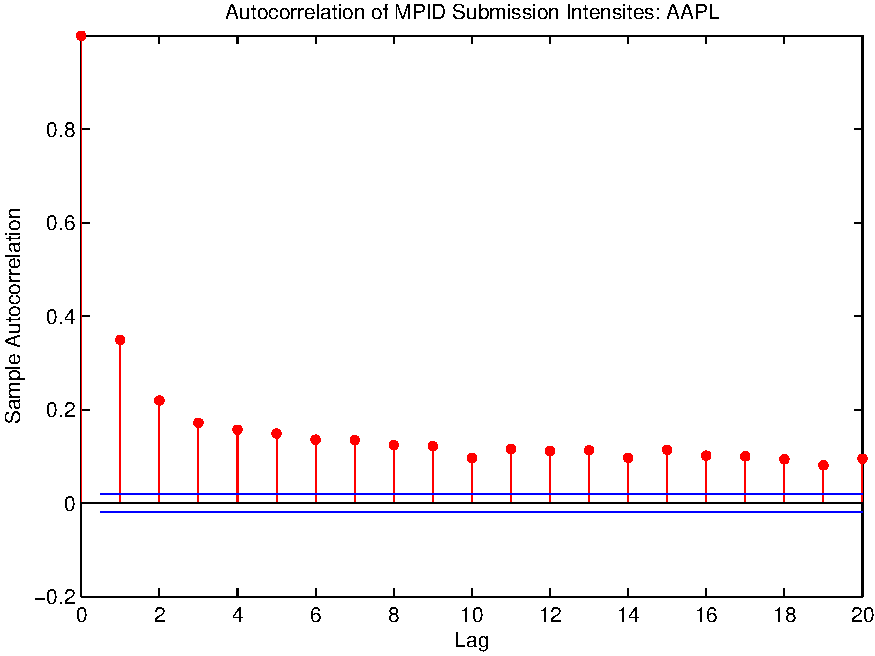
\includegraphics[width=\linewidth]{docs/Graphs_MPID_SUB_RATIO_AAPL_30sec_FullTime.pdf}
%\caption{\tiny Caption} \label{fig:fig1a}
\end{subfigure}
\hspace*{\fill}
\begin{subfigure}{0.24\textwidth}
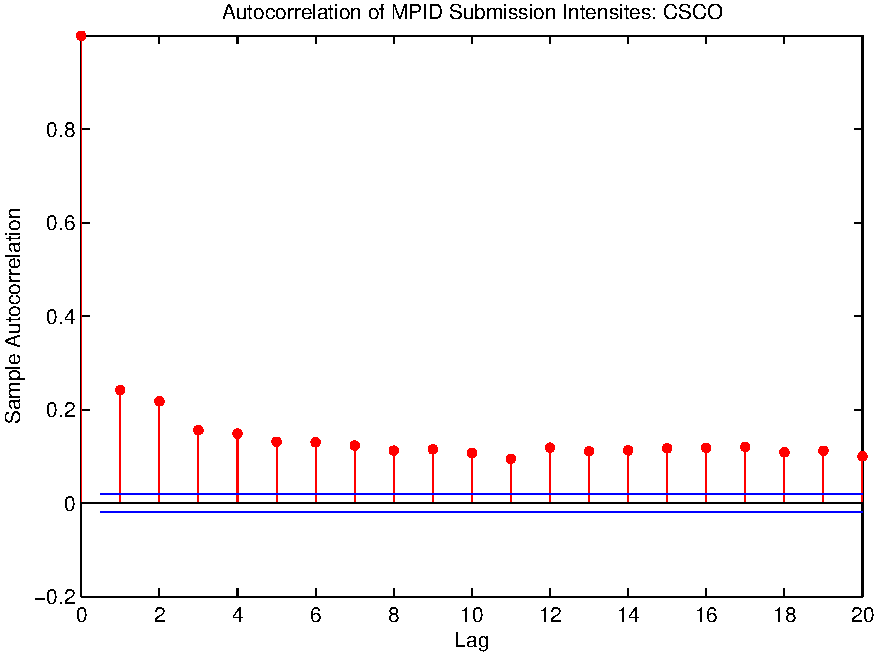
\includegraphics[width=\linewidth]{docs/Graphs_MPID_SUB_RATIO_CSCO_30sec_FullTime.pdf}
%\caption{\tiny Caption} \label{fig:fig1b}
\end{subfigure}
\begin{subfigure}{0.24\textwidth}
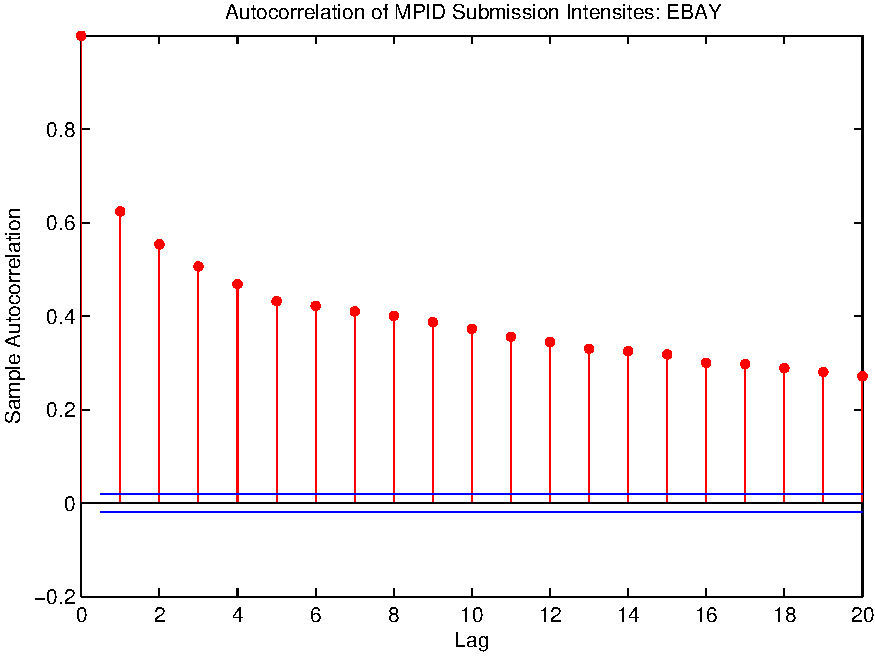
\includegraphics[width=\linewidth]{docs/Graphs_MPID_SUB_RATIO_EBAY_30sec_FullTime.pdf}
%\caption{\tiny Caption} \label{fig:fig1c}
\end{subfigure}
\begin{subfigure}{0.24\textwidth}
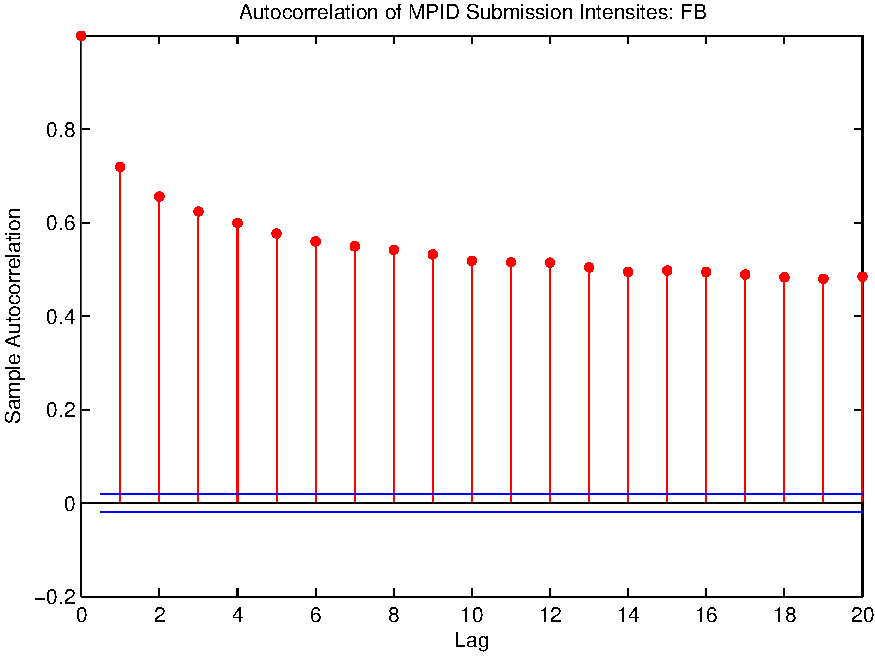
\includegraphics[width=\linewidth]{docs/Graphs_MPID_SUB_RATIO_FB_30sec_FullTime.pdf}
%\caption{\tiny Caption} \label{fig:fig1g}
\end{subfigure}

\begin{subfigure}{0.24\textwidth}
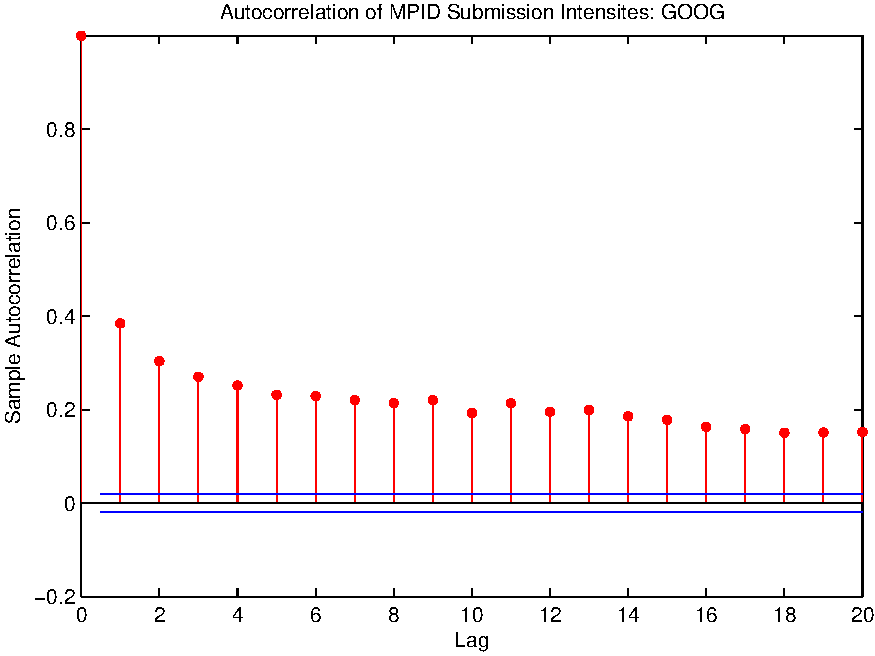
\includegraphics[width=\linewidth]{docs/Graphs_MPID_SUB_RATIO_GOOG_30sec_FullTime.pdf}
%\caption{\tiny Caption} \label{fig:fig1a}
\end{subfigure}
\hspace*{\fill}
\begin{subfigure}{0.24\textwidth}
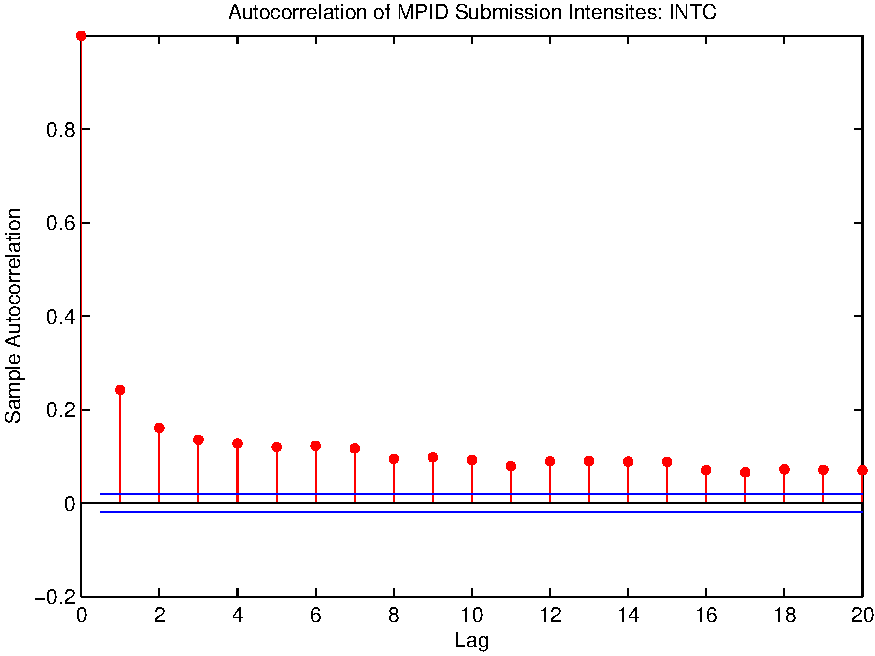
\includegraphics[width=\linewidth]{docs/Graphs_MPID_SUB_RATIO_INTC_30sec_FullTime.pdf}
%\caption{\tiny Caption} \label{fig:fig1b}
\end{subfigure}
\begin{subfigure}{0.24\textwidth}
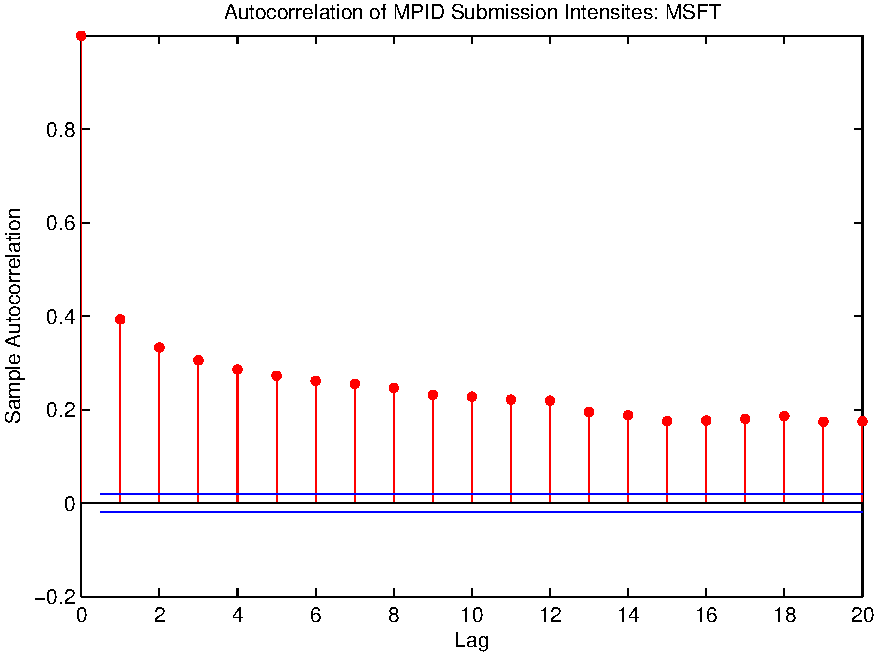
\includegraphics[width=\linewidth]{docs/Graphs_MPID_SUB_RATIO_MSFT_30sec_FullTime.pdf}
%\caption{\tiny Caption} \label{fig:fig1c}
\end{subfigure}
\begin{subfigure}{0.24\textwidth}
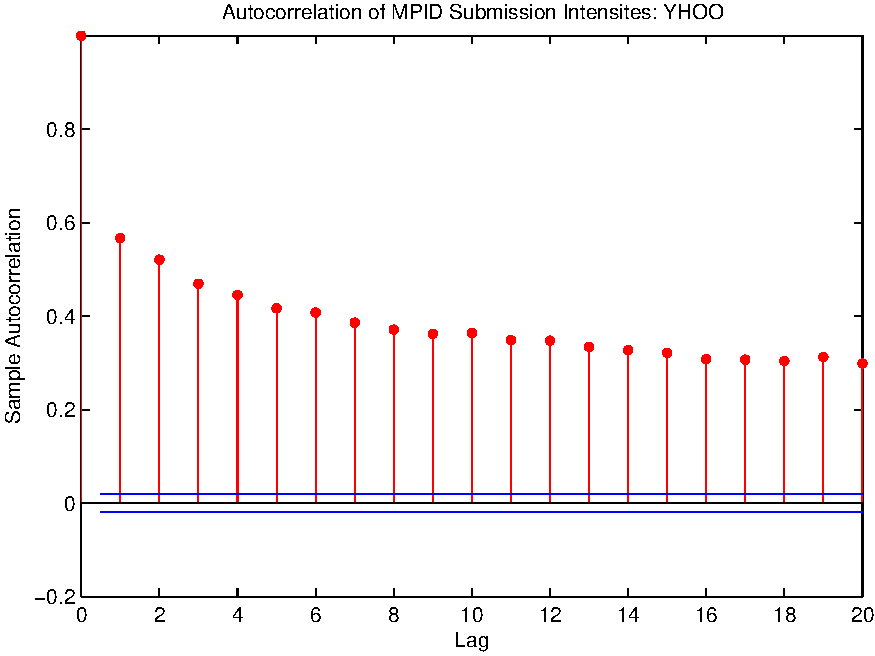
\includegraphics[width=\linewidth]{docs/Graphs_MPID_SUB_RATIO_YHOO_30sec_FullTime.pdf}
%\caption{\tiny Caption} \label{fig:fig1g}
\end{subfigure}
\begin{minipage}{\textwidth}
\footnotesize
Caption
\end{minipage}
\end{figure}

\begin{figure}[htp!]
\caption{Average Daily MPID Submission Ratios, by Firm}\label{ratiostats1}
\begin{center}
\begin{subfigure}{0.45\textwidth}
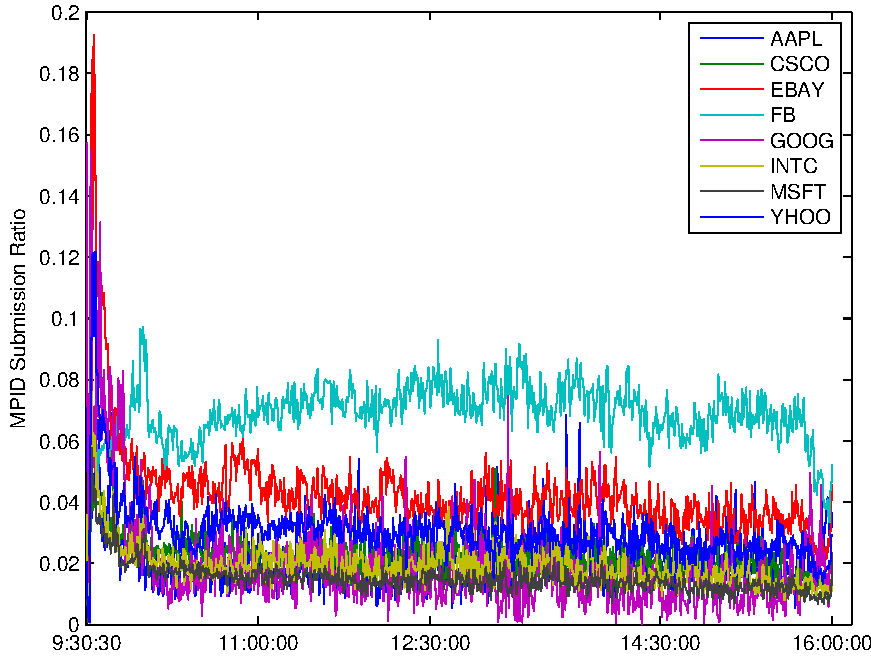
\includegraphics[width=\linewidth]{docs/MPIDSubmission_Daily_ByFirm_30sec_FullTime.pdf}
\end{subfigure}
\begin{subfigure}{0.45\textwidth}
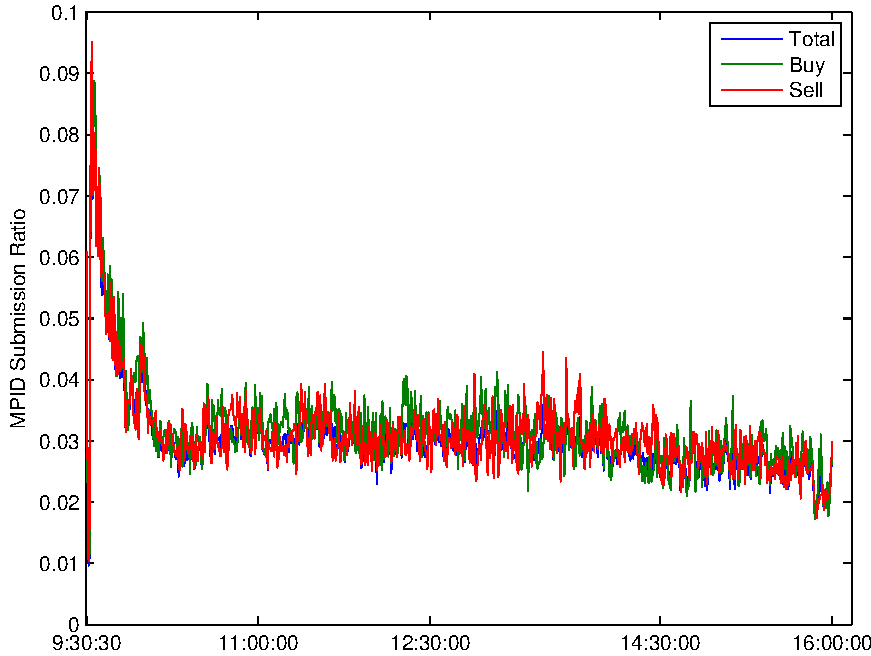
\includegraphics[width=\linewidth]{docs/MPIDSubmission_Daily_ByType_30sec_FullTime.pdf}
\end{subfigure}
\end{center}
\begin{minipage}{\textwidth}
\footnotesize
Caption
\end{minipage}
\end{figure}

\section{Determinants of MPID Order Submissions}\label{determinants}

\subsection{Methodology}\label{method1}

In the first step of our analysis, we would like to examine whether market makers submit MPID-attributed orders in their capacity as liquidity providers, in order to meet liquidity demand and/or stabilize uncertain markets. Therefore, we would like to know the marginal contribution that various market characteristics have on the rate at which MPID-attributed orders are submitted. To achieve this, we perform a panel regression of the MPID-attributed submission intensities on lagged market conditions hypothesized to influence the decision to submit MPID-attributed orders as described in Section \ref{hypothesis}. Specifically, we estimate:

\begin{equation}
MPID_t^i=\alpha_0^i + \sum_{p=1}^5 \alpha_p MPID_{t-p}^i +\alpha_6 OPEN_t + \beta' \textbf{x}_t^i + \gamma' \textbf{z}_t^i + \delta' DAY_t +\varepsilon_{t}^i, \label{prepanel}
\end{equation}

\noindent where $MPID_t^i$ is a variable intended to capture the intensity of MPID-attributed submissions over the interval $[t,t+1]$ (as described in the previous Section \ref{mpidsub}), $\textbf{x}_t^i$ is a vector containing the average order characteristics of MPID-attributed orders submitted over the interval $[t,t+1]$, such as average order size, and $\textbf{z}_t^i$ is a vector containing various market conditions averaged over the interval $[t-1,t]$ that are hypothesized to influence the decision to submit MPID-attributed orders, such as volatility and the bid-ask spread. To account for the high autocorrelation of MPID submission , $p=5$ lags of the dependent variable, $MPID_{t-p}^i$, are included as additional regressors.\footnote{Recall from Section~\ref{mpidsub} the high degree of autocorrelation detected in the MPID submission ratio time series. Therefore, $p=5$ lags are chosen as the number of lags at which there is no more autocorrelation in the error terms of the regressions when tested on a stock-by-stock basis. Durbin-Watson statistics close to 2 are considered generally to confirm no autocorrelation in the errors \citep[see, e.g.,][]{gujarati2004basic}; the average Durbin-Watson statistic across firms is equal to 2.014. Furthermore, the addition of lags implies that we have a \emph{dynamic panel regression}, which potentially introduces bias into the estimates, which can be corrected using, e.g., the GMM procedure of \citet{arellano1991some}. However, this bias $\rightarrow 0$ as $T \rightarrow \infty$. As we have a long time series ($T=10,920$ intervals) and rather short cross-section ($n=8$), our estimates should still be consistent \citep[see, e.g.,][p. 135]{baltagi2008econometric}.} $OPEN_t$ is a dummy variable equal to one if the interval $[t,t+1]$ is within the first thirty minutes of the trading day, and $DAY_t$ is a vector of dummy variables controlling for daily fixed effects. Firm fixed effects are captured by $\alpha_0^i$; results are presented for specifications both including and excluding daily and firm fixed effects. In different specifications, $MPID_t^i$ is defined as the buy- and sell-side MPID submission ratios, as well as the total MPID submission ratio. Additional robustness checks look at the coefficient values from running the panel regression in (\ref{prepanel}) as a time series regression on a stock-by-stock basis, and also look at the behaviour of an individual market maker (the largest market maker in our sample, Timber Hill, LLC) to minimize possible noise from different market makers following different strategies.

The vector of order characteristics, $\textbf{x}_t^i$, contains two variables: the average aggressiveness of MPID-attributed orders over the interval $[t,t+1]$, $AGGR.MPID_t^i$ defined as the signed distance of a submitted order to the midquote, and the average order size (in dollar volume) of MPID-attributed submissions over the interval $[t,t+1]$, $ORSZ.MPID_t^i$. These variables are included to control for the potential that a higher intensity of MPID orders may be driven by, e.g., order-splitting strategies or by ``hiding" attributed orders deep in the book.

The vector $\textbf{z}_t^i$, contains nine lagged variables meant to capture market conditions that are hypothesized in Section \ref{hypothesis} to influence market makers' decision to submit MPID-attributed orders: relative quoted bid-ask spreads ($RELSPR_{t-1}^i$), volatility ($VOL_{t-1}^i$), submission dollar volume ($SUB_{t-1}^i$), execution dollar volume ($EXE_{t-1}^i$), and depth ($DEPTH_{t-1}^i$). These variables are all averaged (or summed in the case of submissions and executions) across the interval $[t-1,t]$. Also included are (unsigned) relative changes in the midquote over the interval $[t-1,t]$ ($RELDPR_{t-1}^i$), a dummy variable equal to one is this relative price change is negative ($NEG.DUMMY_{t-1}^i$), and the interaction between these variables to capture the effects of large, negative changes in prices ($RELDPR_{t-1}^i \times NEG.DUMMY_{t-1}^i$). An alternative specification looks at the effect of positive changes in the prices, $POS.DUMMY_{t-1}^i$. Lastly, we include the Hasbrouck measure, $HASBROUCK_{t-1}^i$, which uses a VAR approach to measure pricing errors as the stationary component of prices after separating out the random walk component. Similarly to in \citet{rosch2017dynamics}, these pricing errors are taken as the maximum measure over the interval $[t-1,t]$. For more details on how these variables are calculated, see Appendix~\ref{sec:measures}.

Similarly to the calculation of $MPID_t^i$ as described in Section~\ref{mpidsub}, all regressors are calculated across 30-second intervals, giving us a time-series dimension of $t=10,920$ (i.e., 780 intervals per day over 14 trading days). Descriptive statistics of the order and market characteristics are presented in Table~\ref{regressstats}. In order to see if MPID-attributed orders differ in terms of their characteristics, the average aggressiveness and order size of all anonymous orders are also presented. The summary statistics reveal some interesting characteristics of MPID-attributed orders. Negative mean and median MPID-attributed order aggressiveness reveals that market makers tend to submit MPID-attributed orders deeper than the first level of the limit order book, and comparing them with anonymous orders reveals that they may be less aggressive on average. Furthermore, comparing MPID-attributed with anonymous orders in terms of size reveals that MPID-attributed orders may be larger on average (both in terms of mean and median order sizes). Furthermore, the highly positive skew on MPID-attributed order sizes perhaps reveals the presence of a few very large MPID-attributed order submissions. Before estimating the panel regression, all variables (excluding the dummies) in the stock-level regressions and in the panel regression in (\ref{prepanel}) are standardized by the stock-level standard deviation, in order to control for differences in regressor magnitudes across stocks and ease interpretation of the coefficients.

\begin{table}[htp!]
\caption{Summary Statistics for Market Condition and Order Characteristic Variables}\label{regressstats}
\begin{center}
\resizebox{0.75\linewidth}{!}{%
\begin{tabular}{lp{1.5cm}p{1.5cm}p{1.5cm}p{1.5cm}p{1.5cm}p{1.5cm}p{1.5cm}} \hline \hline \\
& (1) & (2) & (3) & (4) & (5) & (6) \\ \\
& MEAN               & MEDIAN     & STDEV      & MIN        & MAX     & SKEWNESS           \\
RELSPR             & 0.035   & 0.032   & 0.013   & 0.003  & 0.226     & 1.396  \\
VOL & 0.218   & 0.071   & 0.588   & 0.000  & 31.985    & 13.897 \\
AGGR.MPID      & -0.078  & -0.068  & 0.057   & -0.804 & 0.079     & -1.262 \\
AGGR.ANON & -0.041	& -0.037&	0.018	&-0.188&	0.021&	-1.221  \\
ORSZ.MPID     & 0.025   & 0.007   & 0.065   & 0.000  & 2.970     & 15.504 \\
ORSZ.ANON & 0.011&	0.030&	0.001&	0.359&	2.931 \\
SUB.ALL   & 5.874   & 3.483   & 7.531   & 0.000  & 374.183   & 5.100  \\
EXE.ALL      & 0.519   & 0.197   & 1.100   & 0.000  & 67.423    & 12.872 \\
SUB.BUY       & 2.996   & 1.653   & 4.110   & 0.000  & 107.886   & 4.278  \\
EXE.BUY      & 0.253   & 0.074   & 0.555   & 0.000  & 20.012    & 8.122  \\
SUB.SELL     & 2.877   & 1.612   & 4.105   & 0.000  & 366.986   & 11.945 \\
EXE.SELL     & 0.266   & 0.072   & 0.705   & 0.000  & 63.447    & 20.900 \\
DEPTH.TOTAL & 0.402   & 0.235   & 0.447   & 0.004  & 22.704    & 7.341  \\
DEPTH.BUY    & 0.200   & 0.111   & 0.236   & 0.001  & 6.949     & 5.286  \\
DEPTH.SELL   & 0.202   & 0.112   & 0.288   & 0.001  & 22.465    & 18.798 \\
RELDPR        & 0.000   & 0.000   & 0.047   & -0.801 & 0.749     & 0.144  \\
HASBROUCK     & 0.312   & 0.126   & 0.832   & -4.435 & 48.357    & 15.542 \\
\\
\hline \hline
\end{tabular}}
\begin{minipage}{0.75\textwidth}
\footnotesize
This table shows summary statistics for the order characteristic and market condition variables. Relative bid-ask spreads (RELSPR), relative price changes (RELDPR), aggressiveness of MPID-attributed orders (AGGR.MPID), and pricing errors (HASBROUCK) are scaled by $10^3$. Volatility (VOL) is scaled by $10^6$. Total, buy-side, and sell-side submission and execution volumes and depth, as well as MPID-attributed order sizes (ORSZ.MPID), are expressed as dollar volumes and scaled by $10^{-6}$.
\end{minipage}
\end{center}
\end{table}

\subsection{Empirical Results}\label{results1}

This section presents results from the panel regression as described in Section~\ref{method1}, which examines the marginal impact that various market conditions have on the decisions by market makers to submit MPID-attributed orders. As laid out in Hypothesis 1, if MPID-attributed orders are indeed submitted by market makers in their capacity as liquidity providers, then we should see an increase in MPID submission in response to an imbalance between submission and execution volumes, lower depth, higher volatility, and higher bid-ask spreads. Furthermore, if MPID-attributed orders are submitted by market makers in their capacity as ``contrarian traders", in order to reduce price uncertainty and correct pricing errors, then we might see a higher MPID-attributed order submission ratio correspond to a higher level of aggressiveness, as well as in response to higher pricing errors as measured by the \citet{hasbrouck1993assessing} measure.

Table~\ref{panelMPID} shows results from the panel regression estimation in (\ref{prepanel}). Columns 1-3 show results in which the dependent variable is defined as the total MPID submission intensity, $MPID_t^i$. Panel 1 shows results from an OLS pooling panel regression, excluding firm and time fixed effects. Column 2 includes firm fixed effects, while Column 3 additionally includes day dummies $DAY_t^i$ capturing daily time fixed effects. Column 4 replaces the dummy variable capturing negative prices changes, $NEG.DUMMY_t^i$, with a dummy variable capturing positive price changes, $POS.DUMMY_t^i$, to check if market makers respond differently to large, downward vs. upward price movements. Lastly, in order to see if buy- and sell-side MPID submission vary in terms of their reactions to different sides of the book, the panel regression in (\ref{prepanel}) is further specified to consider the buy- and sell-sides of the book separately. Columns 5-6 show results from specifications in which the dependent variable is defined as, respectively, buy-side MPID submission intensity, $MPID.BUY_t^i$, and sell-side MPID submission intensity, $MPID.SELL_t^i$, including firm and daily time fixed effects. Buy- and sell-side submission volumes are subsequently regressed on same-side submission and executions volumes and depth.

The results broadly support Hypothesis 1, in that market makers indeed submit MPID-attributed orders within the capacity of a liquidity provider. However, the results are more consistent with the idea that market makers submit MPID-attributed orders in order to meet demand from market orders according to the ``reliable counterparties" hypothesis, rather than to stabilize pricing errors according to the ``contrarian trader" hypothesis.

First, the results show that market makers tend to intervene using MPID-attributed orders following periods of high volatility and high relative bid-ask spreads. Positive and significant coefficients (at least at a $\alpha<10\%$ significance level) on lagged volatility, $VOL_{t-1}^i$ reflect that MPID submission ratios tend to be higher following intervals of high volatility: a one-standard-deviation increase in volatility leads to a marginal increase in MPID submissions in the next period of about one basis point (a relative increase of about 2-4\%). \footnote{Note from Table \ref{mpidsubstats} that the standard deviation of $MPID_t^i$ is between 0.031 and 0.040, depending on whether it is defined according to the buy-side, sell-side, or both sides of the book. Since we standardize variables by dividing by the standard deviation, regression coefficients can be interpreted as the marginal increase in standard deviation units of the dependent variable associated with a one-standard deviation increase in the regressor.} Likewise, coefficients on lagged relative quote bid-ask spreads, $RELSPR_{t-1}^i$, are also positive and significant ($\alpha<10\%$) for most specifications, reflecting a 3-4\% (relative) marginal increase in MPID submission ratios following periods of high bid-ask spreads. However, significance is lost once the sell side of the book is considered. Particularly in terms of magnitude, one of the most important drivers of MPID submission ratios seems to be time-of-day effects. The coefficient on the open dummy, $OPEN_t^i$, reflects that MPID order submission ratios tend to be ceteris paribus 15-24\% higher during the first thirty minutes of the trading day. This reflects that market makers are active in supplying limit orders early in the trading day as limit order books are being filled, and as when uncertainty is high as information revealed through after-hours trading is compounded into prices \citep[see, e.g., ][]{foster1993variations,Gerety01071994}.

Furthermore, the results show that market makers tend to intervene using MPID-attributed orders following periods of low submission volume. The negative and significant coefficient on submission volume across all specifications ($\alpha<1\%$) shows that MPID submission ratios tend to be higher following periods of low submission volume, on both sides of the book. In terms of magnitude, a one-standard-deviation decrease in submission volume is followed by up to a $6\%$ relative increase in the MPID submission ratio. Coefficients on execution volume are largely insignificant, but show some evidence that MPID submission ratios tend to be higher following periods of high execution volume. Coefficients on depth are negative and significant (except for sell-side MPID orders), confirming from Hypothesis 1 that MPID order submission ratios increase following intervals of low depth.

However, note that the coefficient on relative price changes $RELDPR_{t-1}^i$ is negative and significant across all specifications. Taken along with the results for volatility, the implication is the market makers respond with MPID-attributed orders following intervals of high variations in price, but actually \emph{reduce} their MPID exposure when prices are moving in a consistent direction. The coefficient on the interaction term between $RELDPR_{t-1}^i$ and the dummy variables capturing the directions of prices changes ($NEG.DUMMY_{t-1^i}$ and $POS.DUMMY_{t-1^i}$) are mostly insignificant, reflecting that market makers are not more likely to respond to positive vs. negative price changes. Specifically, Column 5 shows that MPID-attributed buy orders do not increase following periods of large, negative price changes, and Column 6 shows that MPID-attributed sell orders actually decrease following large, positive price changes. This provides evidence that market makers do not necessarily take on the role of ``contrarian" traders, at least with their MPID-attributed limit orders. No significance is found for the coefficient on pricing errors, $HASBROUCK_{t-1}^i$. Furthermore, from the negative coefficient on $AGGR.MPID_t^i$, a higher MPID-attributed ratio is associated with a lower level of price aggressiveness, showing that market makers are not necessarily interested in the executions of their orders, e.g., to mean-revert pricing errors. Interestingly, positive coefficients on MPID-attributed order size, $ORSZ.MPID_t^i$, show that a higher MPID-attributed ratio is associated with larger orders in terms of volume, which rules out that market makers follow order splitting strategies in submitting MPID-attributed orders.

Overall, the panel regressions provide evidence that, in support of Hypothesis 1, market makers tend to submit a higher intensity of MPID-attributed orders following periods of high volatility, high relative-bid ask spreads, and low submission volume. However, the low aggressiveness of orders and lack of significance response to pricing changes and errors indicates that market makers tend to follow a liquidity provision strategy more akin to that of ``reliable counterparty", rather than ``contrarian trader", in submitting their MPID-attributed orders.

%\subsubsection{Robustness: Stock-Level Regressions}

In order to see if our main results are robust at the individual stock level, Figure~\ref{indreg1} plots the coefficients of MPID submission ratios regressed on the market condition variables of interest, for individual stock-level regressions. In other words, instead of the panel regression in (\ref{prepanel}), time-series regressions are separately run for each individual stock $i$. These regressions include the same explanatory and control variables as described in Section \ref{method1}. The regressions are similarly specified to include daily dummies, $DAY_t$, and for simplicity only the results from regressions defining the dependent variables as total MPID submission ratios are presented.

Results largely confirm the main results from the panel regressions. Coefficients on volatility are positive across all stocks (although only significant for half of the stocks), while positive and significant coefficients on relative bid-ask spreads for the majority of stocks confirm that MPID submission ratios tend to be higher following intervals of high bid-ask spreads. Likewise, the stock-level regressions confirms that MPID submission ratios are higher following periods of low submission volumes, as the coefficient on $SUB_{t-1}$ is negative and significant for the majority of stocks. Coefficients on execution volume are somewhat more mixed in terms of sign, reflecting the limited significance found from the panel regression. Lastly, also confirms the results from the panel regression, the coefficients on $HASBROUCK_{t-1}$ are largely insignificant, and do not show a consistency in terms of sign.

\begin{figure}[htp!]
\caption{Coefficients from Firm-Level Regressions} \label{indreg1}

\begin{subfigure}{0.31\textwidth}
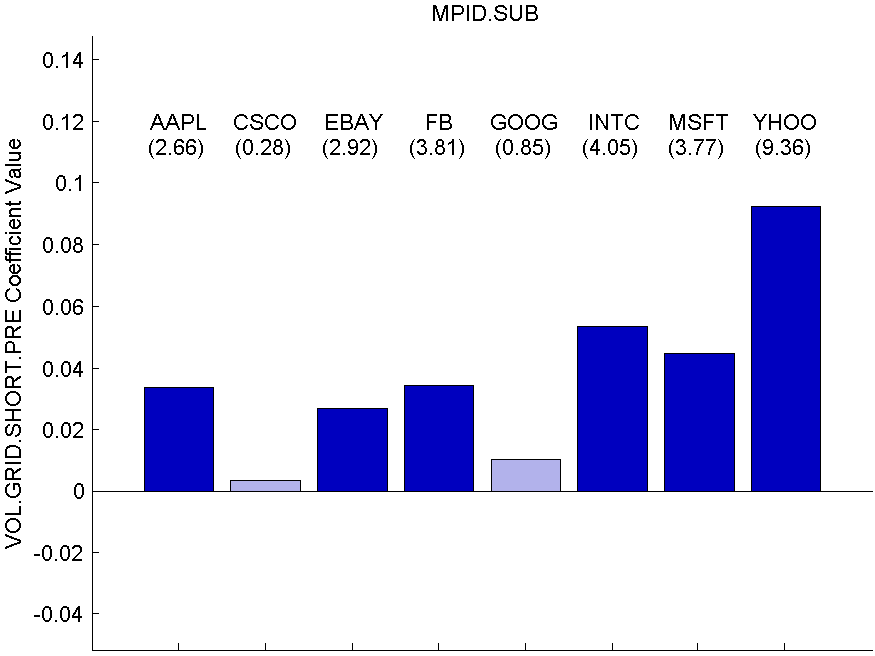
\includegraphics[width=\linewidth]{docs/Regression_Ratio_30sec_1_VOL_GRID_SHORT_PRE.pdf}
%\caption{\tiny Caption} \label{fig:fig1a}
\end{subfigure}
\hspace*{\fill}
\begin{subfigure}{0.31\textwidth}
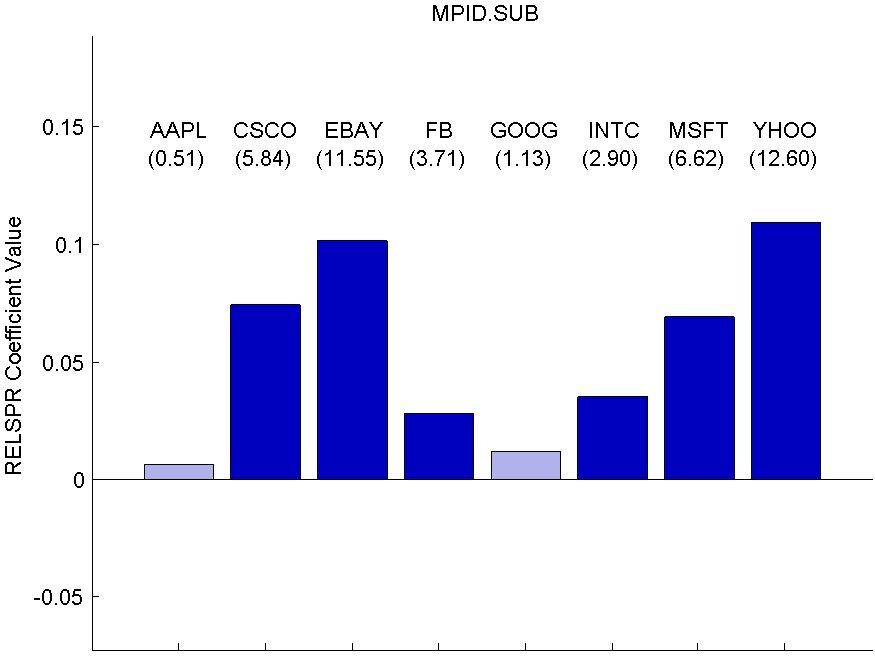
\includegraphics[width=\linewidth]{docs/Regression_Ratio_30sec_1_RELSPR.pdf}
%\caption{\tiny Caption} \label{fig:fig1b}
\end{subfigure}
\begin{subfigure}{0.31\textwidth}
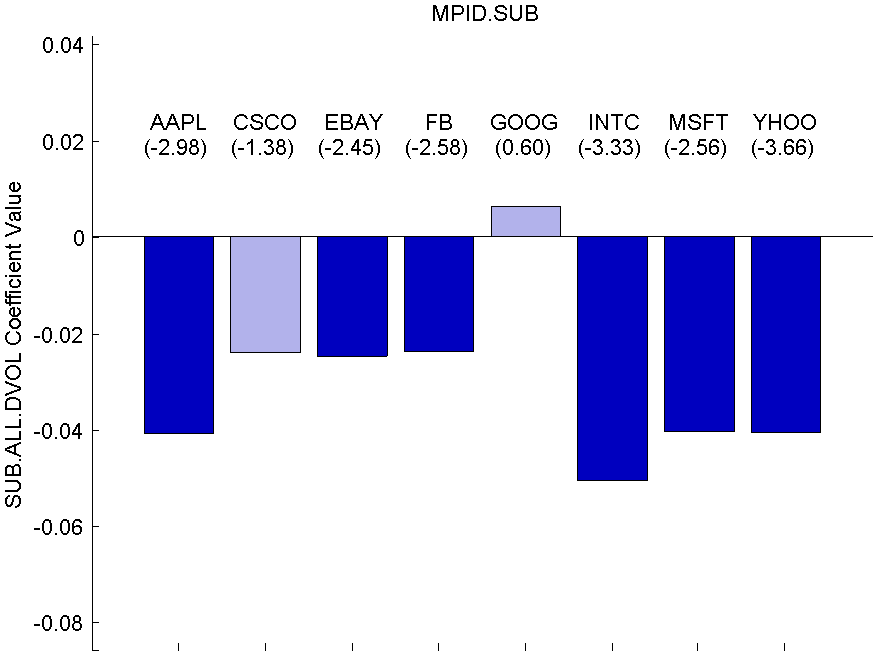
\includegraphics[width=\linewidth]{docs/Regression_Ratio_30sec_1_SUB_ALL_DVOL.pdf}
%\caption{\tiny Caption} \label{fig:fig1c}
\end{subfigure}

\begin{subfigure}{0.31\textwidth}
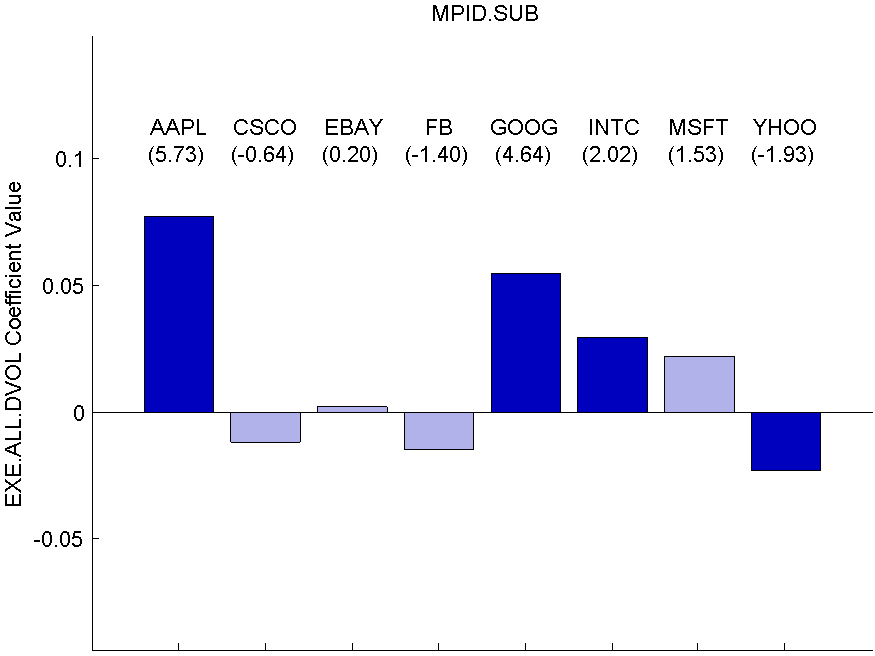
\includegraphics[width=\linewidth]{docs/Regression_Ratio_30sec_1_EXE_ALL_DVOL.pdf}
%\caption{\tiny Caption} \label{fig:fig1g}
\end{subfigure}
\begin{subfigure}{0.31\textwidth}
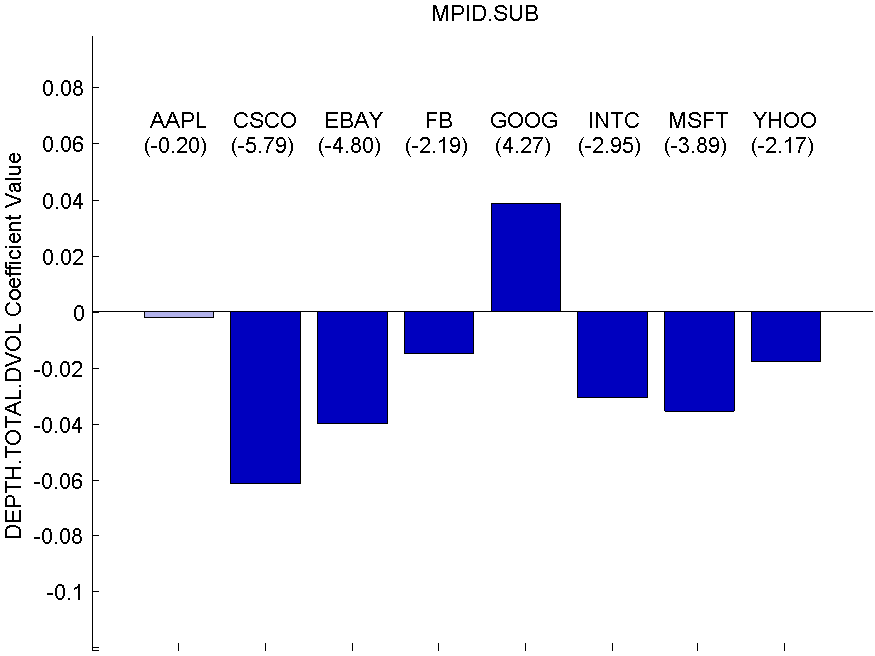
\includegraphics[width=\linewidth]{docs/Regression_Ratio_30sec_1_DEPTH_TOTAL_DVOL.pdf}
%\caption{\tiny Caption} \label{fig:fig1h}
\end{subfigure}
\begin{subfigure}{0.31\textwidth}
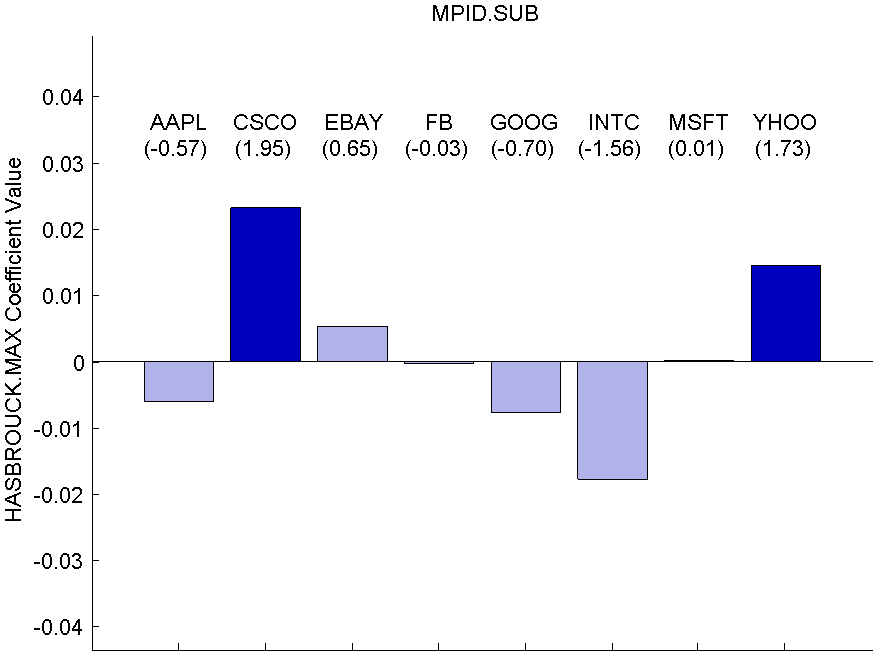
\includegraphics[width=\linewidth]{docs/Regression_Ratio_30sec_1_HASBROUCK_MAX.pdf}
%\caption{\tiny Caption} \label{fig:fig1h}
\end{subfigure}
%\begin{subfigure}{0.31\textwidth}
%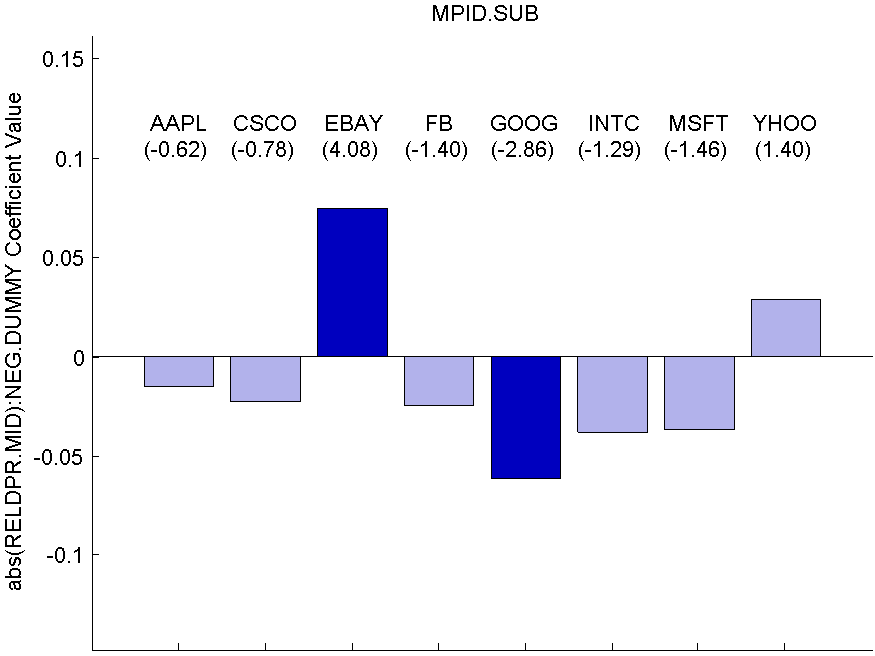
\includegraphics[width=\linewidth]{docs/Regression_Ratio_30sec_1_abs(RELDPR_MID)xNEG_DUMMY.pdf}
%\caption{\tiny Caption} \label{fig:fig1h}
%\end{subfigure}

\begin{minipage}{\textwidth}
\footnotesize
%The bar graphs in the figure above correspond to key coefficients from a regression of measures capturing various dimensions of market quality, on a dummy variable equal to one if a submitted order is attributed to an MPID, and zero otherwise. The dependent variables are calculated during the interval $[t, t+\Delta t]$, where $\Delta t$ is the time it takes to observe $N=20$ consecutive submissions, proceeding the submitted order. Results are presented separately for buy- and sell-side MPID-attributed orders, and separately for each firm in the sample, ordered according to the stock's mean stock price during the sample time period, 4-22 November, from highest to lowest. $t$-statistics are presented in parenthesis above the bar. Dark blue and red bars correspond to coefficients that are significant at a significance level of $\alpha=5\%$. Light blue and red bars correspond to coefficients that are insignificant at this level.
\end{minipage}
\end{figure}

Another robustness check considers that different market makers may have different strategies in terms of MPID attribution. Recall from Table~\ref{tab:mpidnames} that Timber Hill, LLC (MPID: TMBR) accounts for 76.36\% of total MPID submission volume across stocks. This leaves us with a sufficient sample of MPID-attributed orders, in order to consider the determinants of Timber Hill, LLC's placing of TMBR-attributed orders. Therefore, to decrease the potential noise created by aggregating all market makers into one analysis, the panel regression in (\ref{prepanel}) is run, in which the dependent variable is redefined to include only order submissions by Timber Hill, LLC, $TMBR_t^i$. The dependent variable $TMBR_t^i$ thus represents the ratio of the total number of MPID-attributed orders submitted by Timber Hill, to the total number of submitted orders, over the interval $[t,t+1]$.

Results from this panel regression are presented in Table~\ref{panelTMBR}. The results are largely consistent with the results from Table~\ref{panelMPID} using the entire sample of MPID-attributed orders, showing that TMBR-attributed order submissions increase following intervals of high relative bid-ask spreads, high volatility, low submission volume, and low depth. Significance and magnitudes tend to increase, perhaps reflecting a reduction in potential noise from aggregating across market makers. A one-standard-deviation increase in relative bid-ask spreads and volatility implies an increase in the TMBR submission ratio of, resp., 4-6\% and up to $10\%$, in the next interval. A one-standard-deviation decrease in submission volumes implies an increase in MPID-attributed submissions of up to 13\%. The coefficient on pricing errors is insignificant in most specifications, although are positive and significant when fixed effects are excluded.

%\subsubsection{Robustness: Individual Market Maker}

Overall, the findings that MPID-attributed order submissions are higher following intervals of high volatility, high relative bid-ask spreads, low submission volumes, and low depth are rather robust across various specifications, and support the hypothesis that market makers submit MPID-attributed orders within their capacity to provide liquidity. However, the lack of evidence that MPID-attributed orders respond to pricing errors, price changes, and the finding that they tend to be less aggressive, point to the idea that these markets makers are following a role of ``bridging the gap" between buyers and sellers, rather than working to correct pricing errors. The next section explores the extent to which market makers may succeed in generating order flow or stabilizing prices, by exploring whether and how the market reacts to MPID-attributed orders.


\section{Market Reactions to MPID Order Submissions}\label{reactions}

\subsection{Empirical Methodology}\label{method2}

\noindent In this section, we aim to explore the market's reaction to MPID-attributed orders posted by market makers, and the implications that this has for market quality. This approach entails a simple regression of ex-post market quality measures (i.e., measures of market conditions following the submissions of limit orders) on the lagged MPID submission ratio. However, in estimating this regression, we must take into account that, although faced with a quota of non-anonymous order that they must submit, market makers still have discretion over the timing of these orders, and their selection of when to reveal likely depends on the expected costs of doing so. By submitting an MPID-attributed order, for example, when they expect execution volumes to increase, market makers reduce their own exposure to execution risk. Therefore, it would be difficult for an observer to determine whether executions increase as a result of the market maker's submission, or the submission was a result of an expected increase in executions. This introduces a likely endogeneity problem between the market maker's submission decision, and ex-post market conditions. Therefore, in to correct for this potential endogeneity problem, an instrumental variable panel regression is used, in which stock-level MPID order submission ratios are instrumented using the average MPID order submission ratios from the other stocks in our sample. Similar techniques are used in \citet{ComertonForde201570}, \citet{Hasbrouck2013646}, and \citet{buti2011diving}, and follow from the idea that, while MPID-attributed orders submissions in other stocks are likely not driven by the market characteristics in the individual stock, MPID-attributed order submissions are correlated across stocks due to, e.g., trading capacities or constraints of each market makers.

\noindent Consider first a panel regression of ex-post market quality measures on the lagged MPID submission ratio, $MPID_{t-1}^i$. The estimated coefficient on $MPID_{t-1}^i$ thus measures the marginal effect that the submission of an MPID-attributed order has on market quality and market conditions:%
\vspace{-\baselineskip}

\begin{equation}
q_t^{i}=\alpha_0 + \sum_{p=1}^5 \alpha_p q_{t-p}^i + \alpha_6 MPID_{t-1}^i + \alpha_7 SUB_{t-1}^i + \alpha_8 OPEN_t +\beta'\textbf{x}_{t-1}^i+\gamma'\textbf{z}_{t-1}^i+\mu'D_t+\varepsilon_{it}, \label{panel2}
\end{equation}

\noindent where $q_t^{i}$ represents a measure of ex post market quality measured over the interval $[t+1,t]$, such as relative bid-ask spreads or volatility, $\textbf{x}_{t-1}^i$ is a vector controlling for the average order characteristics of MPID-attributed orders submitted over the interval $[t-1,t]$, and $\textbf{z}_{t-1}^i$ is a vector controlling for various market conditions averaged over the interval $[t-1,t]$. Since these measure of market quality tend to also exhibit high degrees of autocorrelation, the regression in (\ref{panel2}) also includes $p=5$ dependent variable lags.\footnote{Durbin-Watson tests statistics confirm a failure to reject a null hypothesis of no autocorrelation in the error terms (tested on a stock-by-stock basis) in the majority of specifications for $q_t^i$, for the majority of firms. The average Durbin-Watson test statistic across specifications and stocks in our case is 1.98.} The key coefficient of interest is the coefficient on lagged MPID order submission intensity, $\alpha_6$, which should give the effect on market quality of an increase in MPID submission intensity. Note that (\ref{panel2}) also controls for changes in the denominator of $MPID_t^i$, i.e., the total submission intensity $SUB.NUM_t^i$. 

%In a first step, the regression in (\ref{panel1}) is run using a standard OLS pooling procedure, including firm fixed effects. In this procedure, we implicity assume no endogeneity between MPID submission intensities and market characteristics. Given the results in [], this is a rather naive assumption, but the results are presented here as Wu-Hausman tests for endogeneity (in which the null) show that OLS is more consistent than 2SLS for at least one of our model specifications (see below).

To account for the endogeneity between MPID submission intensities and market characteristics, we instrument the submission intensity of MPID-attributed orders $MPID_t^{i}$ using the average submission intensities in the other stocks in our sample, $MPID_t^{-i}$. Note that this also requires instrumenting the denominator of $MPID_t^{i}$, $SUB.NUM_t^{i}$ with the average submission intensity of all other stocks, $SUB.NUM_t^{-i}$.

Table~\ref{pearson} shows the Pearson correlation coefficient between the MPID submission ratios in each stock with that of the MPID submission ratios in the other sample stocks, as well as the correlation between each stocks' total submission intensities with the total submission intensities in all other stocks. The table shows a relatively high level of correlation between $SUB.NUM_t^{-i}$ and $SUB.NUM_t^{i}$, with correlation coefficients ranging from 0.19-0.55. Correlation coefficients between $MPID_t^{i}$ and $MPID_t^{-i}$ are also relatively high for six of the stocks, ranging from 0.13-0.447. However, there is nearly zero correlation for AAPL. Therefore, it is possible that $MPID_t^{-i}$ will serve as a weak instrument for this stock.

In order to check this, explicit tests for instrument weakness, as well as tests for the endogeneity of $MPID_t^{i}$ and $SUB.NUM_t^{i}$, are conducted by running two-stage least squares (2SLS) regressions on a firm-by-firm basis. In the first stage, $MPID_t^{i}$ and $SUB.NUM_t^{i}$ are regressed on the instruments $MPID_t^{-i}$ and $SUB.NUM_t^{-i}$, along with the control variables, in order to obtain fitted values $\overline{MPID}_t^{i}$ and $\overline{SUB.NUM}_t^{i}$. In the second stage, $\overline{MPID}_t^{i}$ and $\overline{SUB.NUM}_t^{i}$ are used to substitute for $MPID_t^{i}$ and $SUB.NUM_t^{i}$ in the regression in (\ref{panel2}), estimated on a firm-by-firm basis. A test for weakness of the instruments conducts an $F$-test on the first stage-regressions under the null hypothesis that the instruments is not significant for the first-stage regression. To test for endogeneity of $MPID_t^{i}$ and $SUB.NUM_t^{i}$, a Wu-Hausman test is conducted under the null hypothesis that OLS and 2SLS are equally consistent.

Results for the $F$-tests and Wu-Hausman tests for each stock are presented in Panel B of Table \ref{pearson}, substituting our main market quality measures of interest for $q_t^{i}$ for the dependent variable in regression (\ref{panel2}): relative bid-ask spreads ($RELSPR_t^i$), volatility ($VOL_t^i$), submission volume ($SUB_t^i$), execution volume ($EXE_t^i$), and depth ($DEPTH_t^i$). These results confirm the weakness of $MPID_t^{-i}$ as an instrument for AAPL: the $F$-test fails to reject that $MPID_t^{-i}$ does not enter the first-stage regression at a $\alpha=<10\%$ level for two regressions (relative bid-ask spreads and submission volumes), at a $\alpha<1\%$ for all regressions. Therefore, the proceeding panel regression in which instrumental variable estimation is implemented excludes AAPL from the panel. Interestingly, Panel (E) shows that the Wu-Hausman test fails to reject ($\alpha<5\%$) that OLS is more consistent for two out of the eight firms, when depth ($DEPTH_t^i$) enters as the dependent variable in (\ref{panel2}). 

Similarly to in Section~\ref{method1}, additional robustness checks examine results from (\ref{panel2}) assessed on a stock-by-stock basis, as well as from a regression defining the key regressor of interest as $TMBR_{t-1}^i$, i.e., the ratio of TMBR-attributed orders to the total number of orders submitted during the interval $[t-1,t]$. Furthermore, to see if market conditions also respond to the raw number of MPID-attributed submissions, as well as the ratio of MPID-attributed orders, a further specification replaces the MPID order submission ratio $MPID_{t-1}^i$ with the number of MPID order submissions over the interval $[t-1,t]$, $MPID.NUM_{t-1}^i$.

\subsection{Empirical Results}

This section presents results from the instrumental variable panel regression described in Section~\ref{method2}, which aims to measure the market's reaction to MPID-attributed orders by regressing ex post measures of market quality on lagged MPID submission intensities. According to Hypothesis 2, if the MPID-attributed orders are submitted by market markers in their capacity as liquidity providers, then in response to higher rates of MPID submission we should see higher market participation levels in the form of higher execution and submission volumes. If MPID-attributed orders attract market participation from ``reactive traders", we should see improvements in market quality, such as higher depth, and lower bid-ask spreads and lower volatility. Furthermore, if MPID-attributed orders are submitted by market makers in the capacity as ``contrarian traders" such that their orders are seen by the market as anchoring prices, then in response to higher rates of MPID submission we should see a decrease in pricing errors.

Results are presented in Table~\ref{postpanelMPID}.\footnote{Coefficients on the control variables and lagged dependent variables are suppressed for reasons of space, but full results are available upon request.} Column 1 shows results from an OLS panel regression, including firm and day fixed effects, while Columns 2-5 reflect results using 2SLS estimation. Column 2 excludes day fixed effects, while Column 3 additionally includes includes the day fixed effects $DAY_t^i$. Columns 4 and 5 replace $MPID_t^i$ with $MPID.BUY_t^i$ and $MPID.SELL_t^i$, respectively. Lastly, in order to see if the raw number of MPID-attributed submissions drives ex post market conditions, Column 6 shows results where the regressor of interest is defined as the total \emph{number} of MPID submissions $MPID.NUM_t^i$, as opposed to the ratio of MPID submissions.

The results are somewhat with Hypothesis 2, that market participation rates increase following MPID-attributed market maker orders. However, MPID-attributed orders are not shown to have much of an effect on other measures of market quality by lowering bid-ask spreads or volatility, and are furthermore shown to potentially lead to an increase in pricing errors. This is again more consistent with the ``reliable counterparty" idea of liquidity provision, rather than the ``contrarian trader".

First, Panels A and B show little evidence that MPID submissions have a consistent effect on relative bid-ask spreads and volatility. From Panel A, the coefficients from a regression of $RELSPR_t^i$ on $MPID_{t-1}^i$ show no significance. The one exception is when $MPID_{t-1}^i$ is defined as the \emph{number} of MPID-attributed orders. In this case, relative bid-ask spreads are shown to decrease following intervals of high MPID-attributed submissions; however, significance for this specification is still low. From Panel B, coefficients from a regression of $VOL_t^i$ on $MPID_{t-1}^i$ show more significance, but little consistency in terms of sign. Finally, in contrast to Hypothesis 2b, Panel F shows that intervals of higher MPID-attributed order submissions tend to be followed by an \emph{increase} in pricing errors. Overall, this shows that the revelation of a market maker's presence does not necessarily succeed at ``anchoring" the price and reducing price uncertainty.

On the other hand, Panels C and D generally show an increase in market participation levels following intervals of high MPID-attributed submissions. Panel C shows a positive and significant ($\alpha < 5\%$) coefficient for submission volumes $SUB_t$ across all specifications using the 2SLS instrumental variable estimation. In terms of economic significance, the magnitude of the coefficients point to a 1-3\% increase in submission volumes following a one-standard-deviation increase in MPID submission ratios (5\% increase for an increase in the number of MPID submissions). The strongest results are shown in Panel D, which looks at the impact of MPID submissions on execution volumes. The results show that a significant and positive coefficient for $EXE_t$ across all 2SLS specifications, pointing to a 14-42\% increase in execution volumes following a one-standard deviation increase in MPID submission ratios (55\% increase for an increase in the number of MPID submissions). Note that the coefficient for depth is significant across all specifications; however, it is negative for the OLS estimation and positive for the 2SLS estimations. Given the results from the Wu-Hausman tests from Section~\ref{pearson}, inference for this variable is therefore not straightforward.

Similarly to in Section~\ref{results1}, Figure~\ref{indreg2} plots the coefficients from a 2SLS regression in (\ref{panel2}), estimated on a stock-by-stock basis, in order to see if our main results are robust at the individual stock level. Overall, the results from the stock-level regressions are much noisier. Figure~\ref{indreg2} shows that execution volumes increase significantly for four out of seven stocks, but that they actually \emph{decrease} for two of them. Again, this may be due to noise from aggregating market makers that follow different strategies.

Therefore, a next step looks at both panel regressions and individual stock-level regressions as in (\ref{panel2}), in which the main regressor of interest is redefined to include only order submissions by Timber Hill, LLC, $TMBR_t^i$. Table \ref{panelMPID} shows results for the panel regressions, while Figure \ref{indreg3} plots coefficients from a 2SLS regression estimated on a stock-by-stock basis. Results from the panel regression mostly mirror those from the full sample of market makers, though they show a more significant decrease in relative bid-ask spreads following an increase in TMBR-attributed submissions. Importantly, the main result still holds: a one-standard deviation increase in TMBR submission ratios increases submission volumes by 2-5\% and execution volumes by 13-44\%. The results from stock-level regressions also show more consistency across firms: submissions are shown to increase for four of seven firms, while executions are shown to increase for five of the seven firms. 

Overall, there is little evidence that relative bid-ask spreads and volatility decrease following intervals of high MPID-attributed orders, and pricing errors are furthermore shown to potentially \emph{increase} following intervals of high MPID-attributed orders. Where significant market reactions are found are with variable capturing market participation rates: submission and execution volumes are shown to increase following periods of high MPID-attributed order submissions across nearly all specifications in the panel regression, and are mostly consistent with stock-level results once the noise from aggregating across market makers is reduced.

\begin{figure}[htp!]
\caption{Coefficients from Firm-Level Post Regressions} \label{indreg2}

\begin{subfigure}{0.31\textwidth}
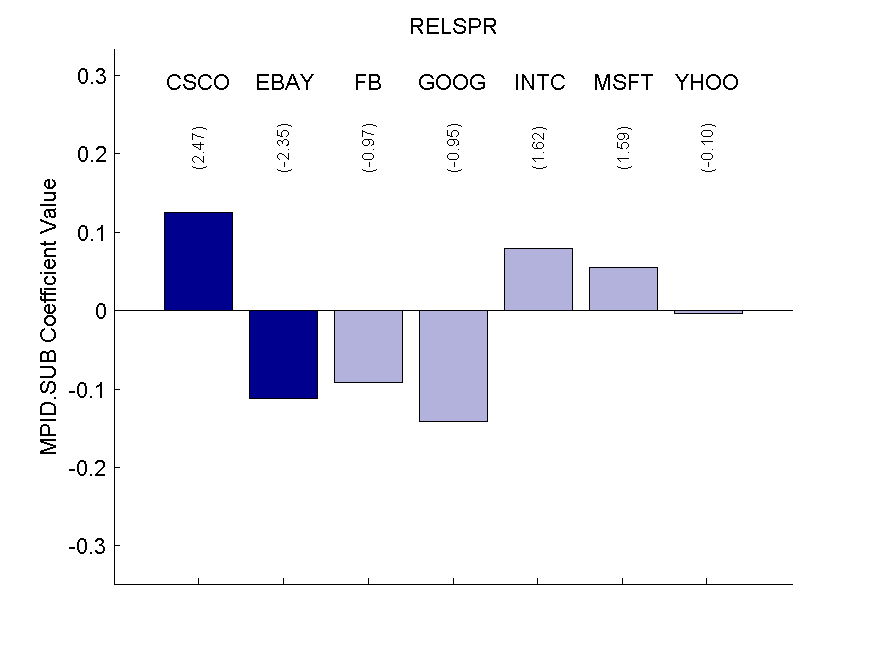
\includegraphics[width=\linewidth]{docs/Regression_Ratio_30sec_1_MPID_SUB_1MPIDLags_5DepVarLags.pdf}
%\caption{\tiny Caption} \label{fig:fig1a}
\end{subfigure}
\hspace*{\fill}
\begin{subfigure}{0.31\textwidth}
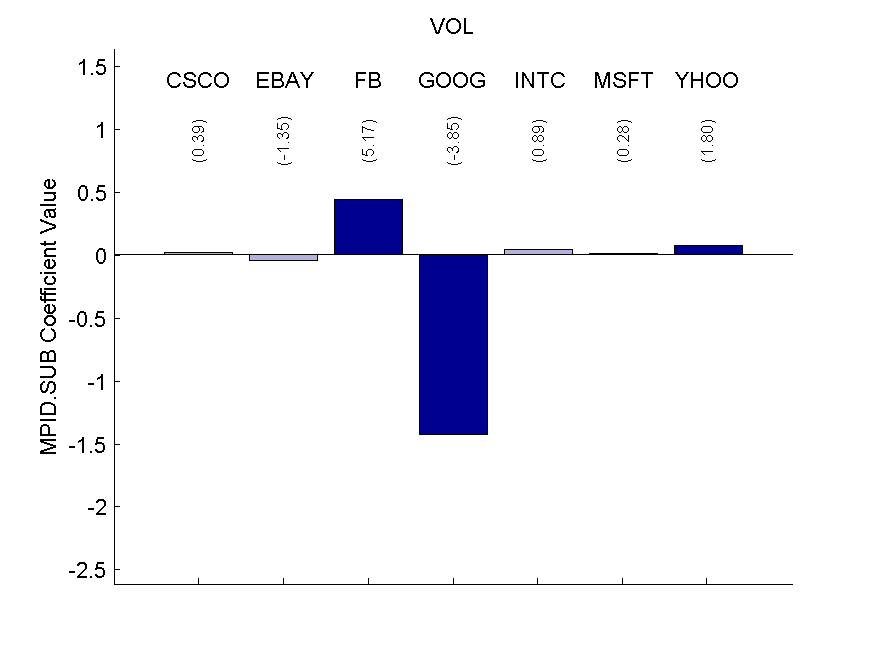
\includegraphics[width=\linewidth]{docs/Regression_Ratio_30sec_6_MPID_SUB_1MPIDLags_5DepVarLags.pdf}
%\caption{\tiny Caption} \label{fig:fig1b}
\end{subfigure}
\begin{subfigure}{0.31\textwidth}
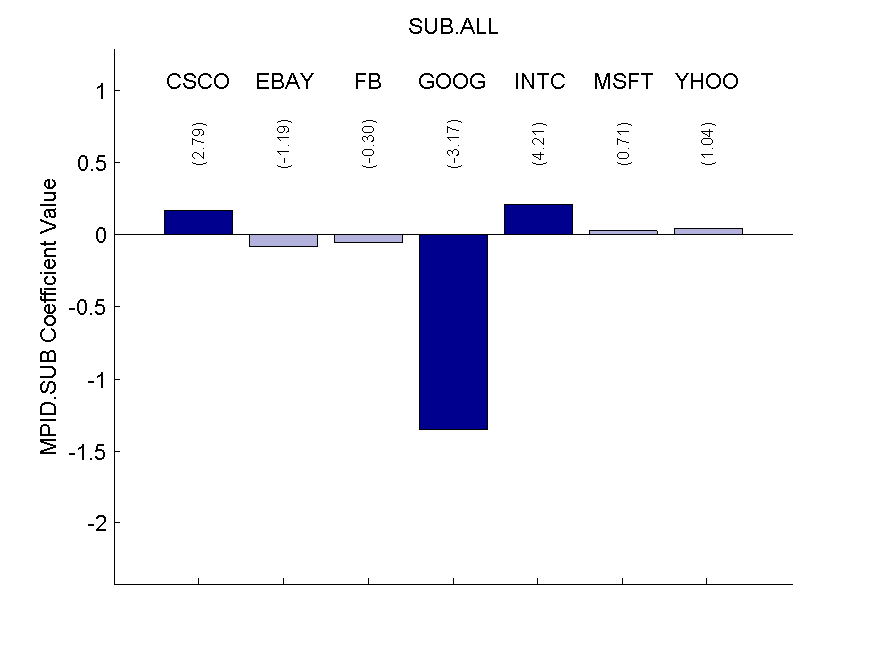
\includegraphics[width=\linewidth]{docs/Regression_Ratio_30sec_11_MPID_SUB_1MPIDLags_5DepVarLags.pdf}
%\caption{\tiny Caption} \label{fig:fig1c}
\end{subfigure}


\begin{subfigure}{0.31\textwidth}
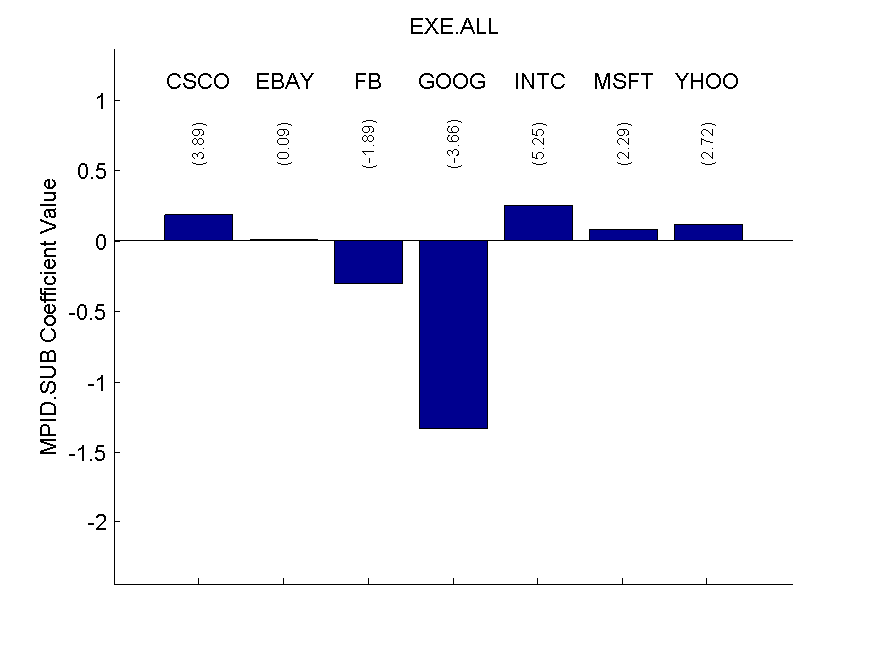
\includegraphics[width=\linewidth]{docs/Regression_Ratio_30sec_16_MPID_SUB_1MPIDLags_5DepVarLags.pdf}
%\caption{\tiny Caption} \label{fig:fig1g}
\end{subfigure}
\begin{subfigure}{0.31\textwidth}
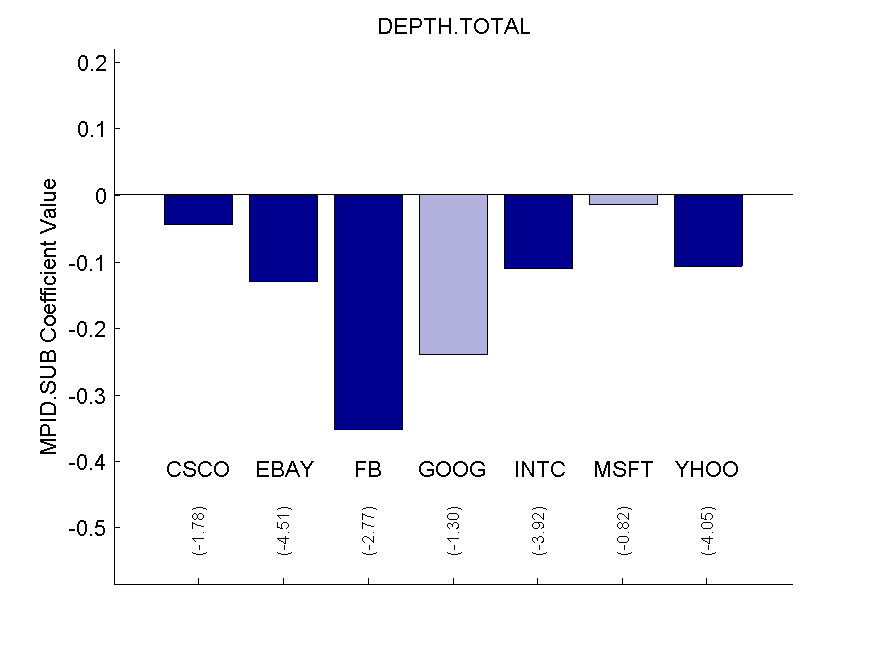
\includegraphics[width=\linewidth]{docs/Regression_Ratio_30sec_21_MPID_SUB_1MPIDLags_5DepVarLags.pdf}
%\caption{\tiny Caption} \label{fig:fig1h}
\end{subfigure}
\begin{subfigure}{0.31\textwidth}
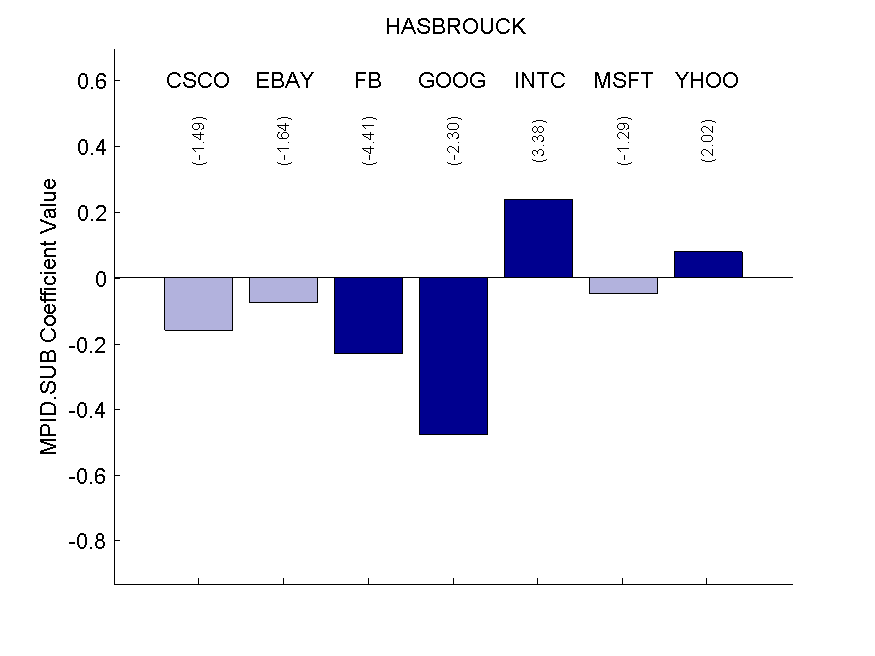
\includegraphics[width=\linewidth]{docs/Regression_Ratio_30sec_26_MPID_SUB_1MPIDLags_5DepVarLags.pdf}
%\caption{\tiny Caption} \label{fig:fig1h}
\end{subfigure}
%\begin{subfigure}{0.31\textwidth}
%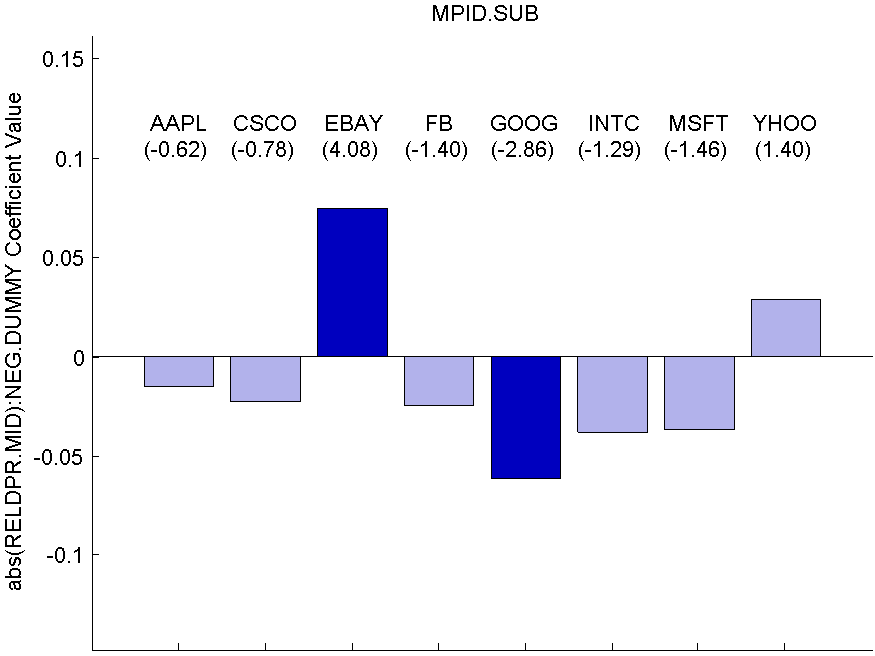
\includegraphics[width=\linewidth]{docs/Regression_Ratio_30sec_1_abs(RELDPR_MID)xNEG_DUMMY.pdf}
%\caption{\tiny Caption} \label{fig:fig1h}
%\end{subfigure}

\begin{minipage}{\textwidth}
\footnotesize
%The bar graphs in the figure above correspond to key coefficients from a regression of measures capturing various dimensions of market quality, on a dummy variable equal to one if a submitted order is attributed to an MPID, and zero otherwise. The dependent variables are calculated during the interval $[t, t+\Delta t]$, where $\Delta t$ is the time it takes to observe $N=20$ consecutive submissions, proceeding the submitted order. Results are presented separately for buy- and sell-side MPID-attributed orders, and separately for each firm in the sample, ordered according to the stock's mean stock price during the sample time period, 4-22 November, from highest to lowest. $t$-statistics are presented in parenthesis above the bar. Dark blue and red bars correspond to coefficients that are significant at a significance level of $\alpha=5\%$. Light blue and red bars correspond to coefficients that are insignificant at this level.
\end{minipage}
\end{figure}

\begin{figure}[htp!]
\caption{Coefficients from Firm-Level Post Regressions: TMBR} \label{indreg3}

\begin{subfigure}{0.31\textwidth}
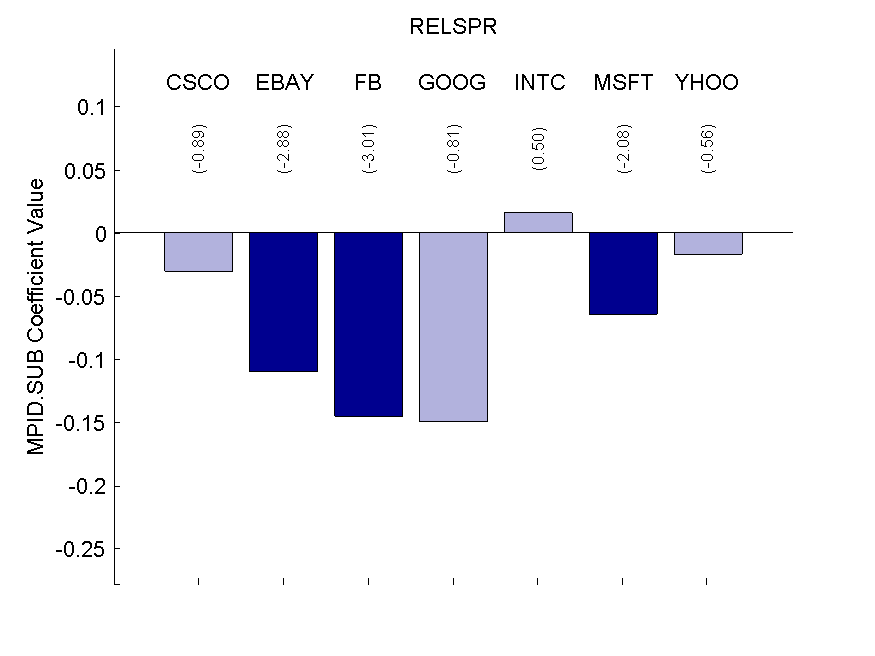
\includegraphics[width=\linewidth]{docs/TMBR_Regression_Ratio_30sec_1_MPID_SUB_1MPIDLags_5DepVarLags.pdf}
%\caption{\tiny Caption} \label{fig:fig1a}
\end{subfigure}
\hspace*{\fill}
\begin{subfigure}{0.31\textwidth}
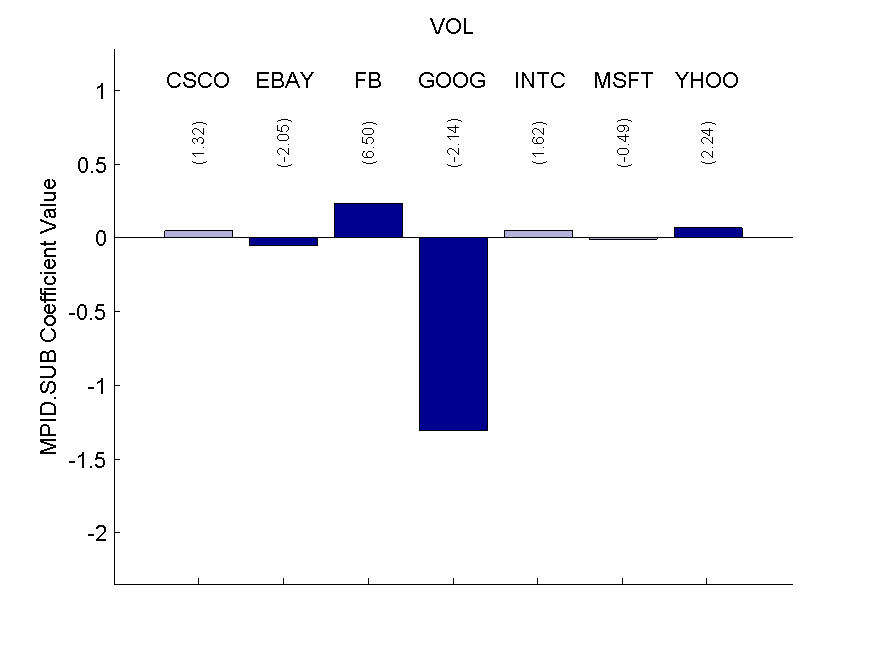
\includegraphics[width=\linewidth]{docs/TMBR_Regression_Ratio_30sec_6_MPID_SUB_1MPIDLags_5DepVarLags.pdf}
%\caption{\tiny Caption} \label{fig:fig1b}
\end{subfigure}
\begin{subfigure}{0.31\textwidth}
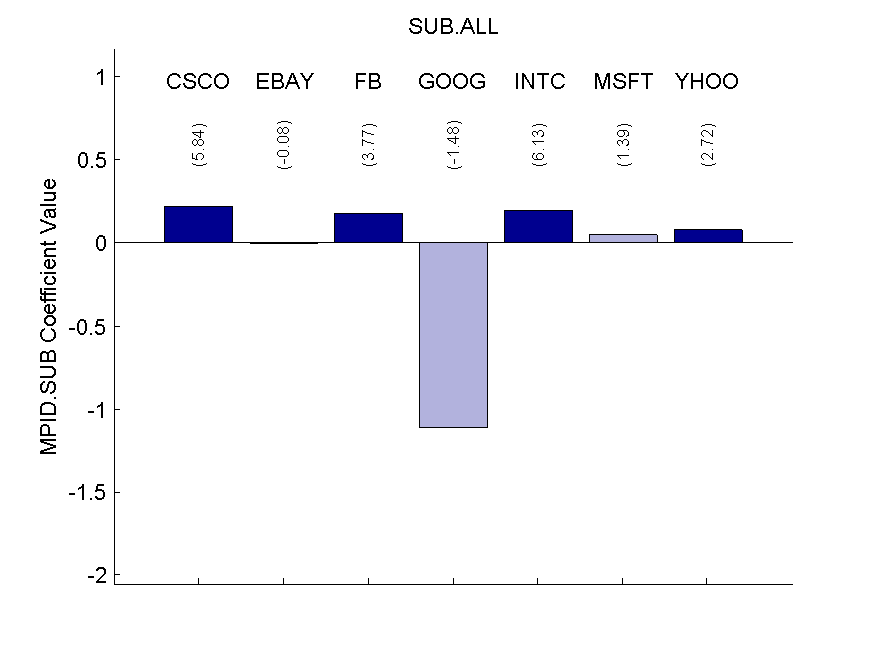
\includegraphics[width=\linewidth]{docs/TMBR_Regression_Ratio_30sec_11_MPID_SUB_1MPIDLags_5DepVarLags.pdf}
%\caption{\tiny Caption} \label{fig:fig1c}
\end{subfigure}


\begin{subfigure}{0.31\textwidth}
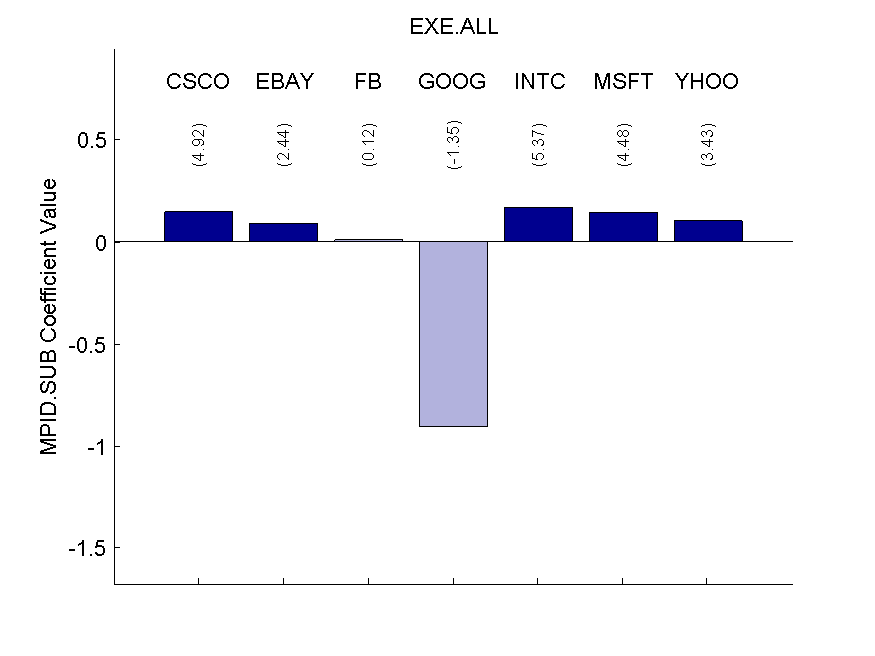
\includegraphics[width=\linewidth]{docs/TMBR_Regression_Ratio_30sec_16_MPID_SUB_1MPIDLags_5DepVarLags.pdf}
%\caption{\tiny Caption} \label{fig:fig1g}
\end{subfigure}
\begin{subfigure}{0.31\textwidth}
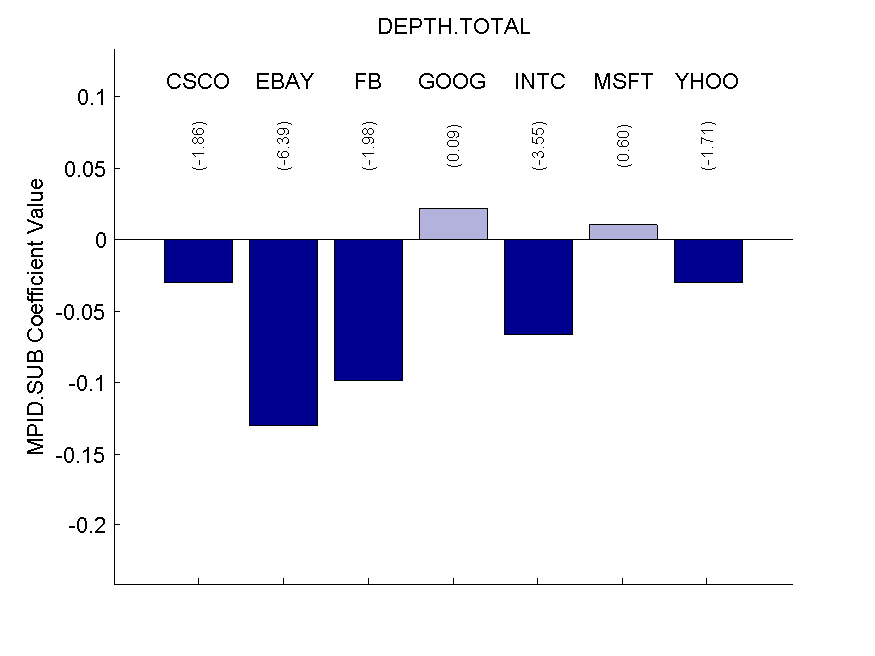
\includegraphics[width=\linewidth]{docs/TMBR_Regression_Ratio_30sec_21_MPID_SUB_1MPIDLags_5DepVarLags.pdf}
%\caption{\tiny Caption} \label{fig:fig1h}
\end{subfigure}
\begin{subfigure}{0.31\textwidth}
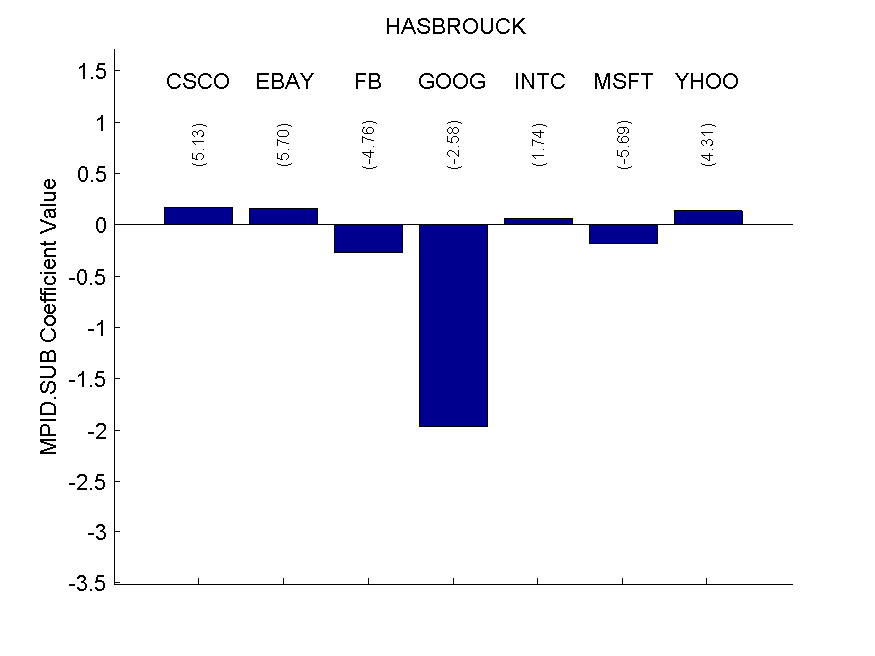
\includegraphics[width=\linewidth]{docs/TMBR_Regression_Ratio_30sec_26_MPID_SUB_1MPIDLags_5DepVarLags.pdf}
%\caption{\tiny Caption} \label{fig:fig1h}
\end{subfigure}
%\begin{subfigure}{0.31\textwidth}
%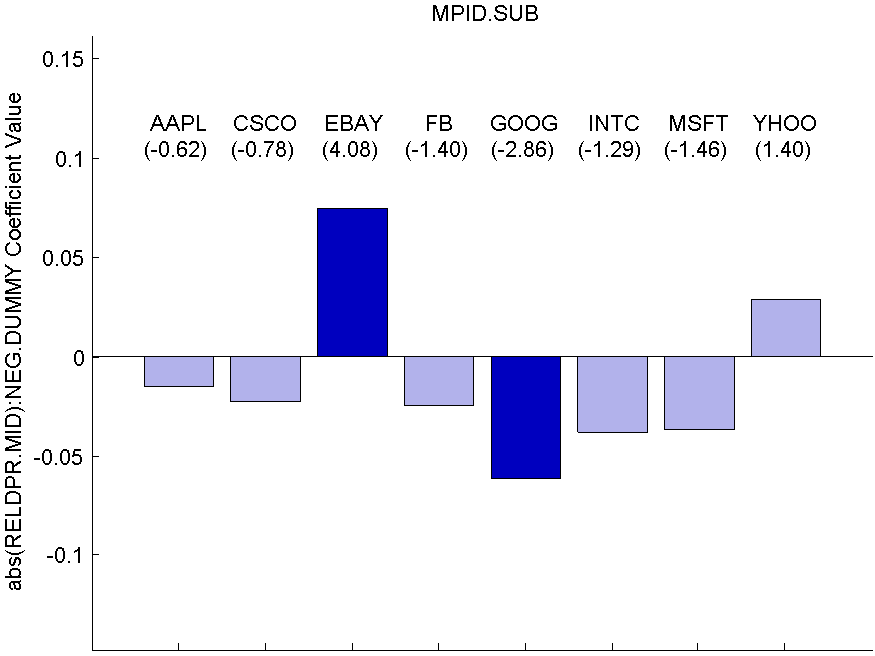
\includegraphics[width=\linewidth]{docs/Regression_Ratio_30sec_1_abs(RELDPR_MID)xNEG_DUMMY.pdf}
%\caption{\tiny Caption} \label{fig:fig1h}
%\end{subfigure}

\begin{minipage}{\textwidth}
\footnotesize
%The bar graphs in the figure above correspond to key coefficients from a regression of measures capturing various dimensions of market quality, on a dummy variable equal to one if a submitted order is attributed to an MPID, and zero otherwise. The dependent variables are calculated during the interval $[t, t+\Delta t]$, where $\Delta t$ is the time it takes to observe $N=20$ consecutive submissions, proceeding the submitted order. Results are presented separately for buy- and sell-side MPID-attributed orders, and separately for each firm in the sample, ordered according to the stock's mean stock price during the sample time period, 4-22 November, from highest to lowest. $t$-statistics are presented in parenthesis above the bar. Dark blue and red bars correspond to coefficients that are significant at a significance level of $\alpha=5\%$. Light blue and red bars correspond to coefficients that are insignificant at this level.
\end{minipage}
\end{figure}

From the results examining market reactions to MPID-attributed orders, MPID-attributed orders appear to encourage market participation, but this increased participation does not seem to bring about an improvement in market quality. This goes along with the idea from \citet{harris1997order} of order exposure potentially attracting participation by ``parasitic traders". Rather than encouraing participation by reactive traders, who wish to trade for exogenous reasons but wait for reliable trading opportunities to appear before acting upon trading intentions, order exposure by market makers may encourage participation from ``parasitic traders", whose trading strategies use the information gleaned from MPID-attributed orders in order to profit. For example, a parasitic traders may view and MPID-attributed order as containing some information about the market maker's inventory, and they may attempt to exploit this information by front-running the MPID-attributed order. As orders by parasitic traders do not provide liquidity or generate information of their own, encouraging trading by such market participants does not necessarily lead to improvements in market quality in terms of lower volatility or spreads or an increased price efficiency.

In their paper on pricing errors, \citet{Hendershott2014405} shows that specialists who act to correct pricing errors at the same time exposure themselves to significant levels of adverse selection. As MPID-attributed orders are already exposed to a high degree of adverse selection through the revelation of trading intensions, market makers may not be willing to go the extra step with their MPID-attributed orders to actively trade against pricing errors. Instead of ``anchoring" the price and encouraging reactive traders, who might help improve market quality by providing their own contr-side liquidity and may contain exogenous information that could improve price efficiency, MPID-attributed orders may encourage the ``wrong" types of traders, who exploit information revealed through MPIDs, without contributing liquidity or information of their own. Therefore, while achieving the classic goal of increased market participation, the requirement that market makers expose a portion of their limit orders may not translate into an overall improvement in market quality.

\section{Conclusion}\label{conclusion}

Since the mid-2000s, technological advances and regulatory changes have largely pushed out the role of traditional market makers, mandated to maintain orderly markets, and led to the rise of endogenous liquidity providers, who provide liquidity on their own accounts without direct obligations. To ensure a smooth and continuous provision of liquidity, Nasdaq and other exchanges have implemented a number of programs, to encourage market participants who register as market makers to fulfill the roles that make market makers invaluable to financial markets: namely, to step in as counterparties when they are scarce, and to stabilize markets when uncertainty is high. On the other hand, such incentive programs mandate that market makers disclose their identities for a certain quota of submissions throughout the trading day. This leaves market makers at a crossroads between fulfilling their obligations as liquidity providers, and avoiding the adverse selection that comes along with order disclosure within highly anonymized electronic markets. Thus, with this paper, we aim to explore whether MPID-attributed orders by market makers are indeed aligned with incentives to act according to these obligations, and the potential implications that this has for market quality in modern-day equity markets.

\noindent Using a unique dataset that contains information on the identities of the market makers who submit orders, our results show that market makers for the most part respond to market conditions in which liquidity provision is needed. They tend to submit higher intensities of MPID-attributed limit orders when relative bid-ask spreads and volatility are high, and when depth and submission volumes are low. However, there is little evidence that market makers submit non-anonymous orders in order to correct pricing errors and stabilize markets. 

\noindent Further results show the implications that this has for market quality. MPID-attributed orders, while shown to increase market participation levels in the form of higher submissions and executions, do not seem to lead to improvements in overall market quality. There is only mixed evidence that these orders lead to reduced bid-ask spreads, lower volatility, and lower pricing errors, while execution volumes in particular are shown to increase considerably.  

%\noindent Our results further show that, internalizing the market's response to their MPID-attributed orders, market makers choose to submit MPID-attributed orders when they expect the impacts of their orders to be minimized. Market makers tend to submit MPID-attributed orders when quoted spreads are low, and are less likely to submit MPID-attributed orders following price changes (both negative and positive). They are also less likely to submit MPID-attributed following increases in opposite-side execution volume; in other words, they avoid contributing additional signals to information flows. Furthermore, MPID-attributed orders also tend to be smaller and less aggressive, to avoid signalling further that the order is informed. These results show that mandates for identity disclosure may constrain market makers more than incentivize them, as they must act to minimize the de-stabilizing impacts of their non-anonymous orders, rather than using them in their capacity to stabilize markets.

\citet{Hendershott2014405} suggest that one way to encourage liquidity provision is by reducing the risk exposure of liquidity providers, as such allowing them to better act to use their inventory positions to correct pricing errors. By requiring market makers to expose themselves to a \emph{higher} level of adverse selection by exposing their identities in highly anonymous markets, the market maker incentive program may thus be counterproductive to this goal. While MPID-attributed order achieve one goal of increasing order executions, these executions may stem from the attraction of ``parasitic traders", and thus lead to an overall lack of improvement in market quality. 



%"for very
%large
%T
%, they argue that individual unit root time series tests"
%\url{https://fvela.files.wordpress.com/2011/10/baltagi-2005-econometric-analysis-of-panel-data-3e.pdf}

\clearpage

\begin{table}[!htbp] \centering
  \caption{Panel Regression Results}
  \label{panelMPID}
\resizebox{0.9\linewidth}{!}{%
\begin{tabular}{@{\extracolsep{5pt}}lp{1.5cm}p{1.5cm}p{1.5cm}p{1.5cm}p{1.5cm}p{1.5cm}}
\\[-1.8ex]\hline
\hline \\[-1.8ex]
 & \multicolumn{6}{c}{\textit{Dependent variable:}} \\
\cline{2-7}
\\[-1.8ex] & \multicolumn{4}{c}{MPID} & MPID.BUY & MPID.SELL \\
\\[-1.8ex] & (1) & (2) & (3) & (4) & (5) & (6)\\
\hline \\[-1.8ex]
% L1.MPID.SUB.RATIO, k = c(1:mpidlags))1 & 0.278$^{***}$ & 0.273$^{***}$ & 0.270$^{***}$ & 0.270$^{***}$ &  &  \\
%  & (0.028) & (0.029) & (0.028) & (0.028) &  &  \\
%  L1.MPID.SUB.RATIO, k = c(1:mpidlags))2 & 0.134$^{***}$ & 0.130$^{***}$ & 0.128$^{***}$ & 0.128$^{***}$ &  &  \\
%  & (0.014) & (0.015) & (0.014) & (0.014) &  &  \\
%  L1.MPID.SUB.RATIO, k = c(1:mpidlags))3 & 0.085$^{***}$ & 0.081$^{***}$ & 0.078$^{***}$ & 0.078$^{***}$ &  &  \\
%  & (0.009) & (0.010) & (0.008) & (0.008) &  &  \\
%  L1.MPID.SUB.RATIO, k = c(1:mpidlags))4 & 0.078$^{***}$ & 0.074$^{***}$ & 0.071$^{***}$ & 0.071$^{***}$ &  &  \\
%  & (0.006) & (0.007) & (0.006) & (0.006) &  &  \\
%  L1.MPID.SUB.RATIO, k = c(1:mpidlags))5 & 0.075$^{***}$ & 0.070$^{***}$ & 0.067$^{***}$ & 0.067$^{***}$ &  &  \\
%  & (0.006) & (0.007) & (0.007) & (0.007) &  &  \\
%  L1.MPID.SUB.BUY.RATIO, k = c(1:mpidlags))1 &  &  &  &  & 0.238$^{***}$ &  \\
%  &  &  &  &  & (0.024) &  \\
%  L1.MPID.SUB.BUY.RATIO, k = c(1:mpidlags))2 &  &  &  &  & 0.117$^{***}$ &  \\
%  &  &  &  &  & (0.012) &  \\
%  L1.MPID.SUB.BUY.RATIO, k = c(1:mpidlags))3 &  &  &  &  & 0.073$^{***}$ &  \\
%  &  &  &  &  & (0.008) &  \\
%  L1.MPID.SUB.BUY.RATIO, k = c(1:mpidlags))4 &  &  &  &  & 0.071$^{***}$ &  \\
%  &  &  &  &  & (0.005) &  \\
%  L1.MPID.SUB.BUY.RATIO, k = c(1:mpidlags))5 &  &  &  &  & 0.066$^{***}$ &  \\
%  &  &  &  &  & (0.007) &  \\
%  L1.MPID.SUB.SELL.RATIO, k = c(1:mpidlags))1 &  &  &  &  &  & 0.242$^{***}$ \\
%  &  &  &  &  &  & (0.026) \\
%  L1.MPID.SUB.SELL.RATIO, k = c(1:mpidlags))2 &  &  &  &  &  & 0.122$^{***}$ \\
%  &  &  &  &  &  & (0.012) \\
%  L1.MPID.SUB.SELL.RATIO, k = c(1:mpidlags))3 &  &  &  &  &  & 0.071$^{***}$ \\
%  &  &  &  &  &  & (0.010) \\
%  L1.MPID.SUB.SELL.RATIO, k = c(1:mpidlags))4 &  &  &  &  &  & 0.069$^{***}$ \\
%  &  &  &  &  &  & (0.008) \\
%  L1.MPID.SUB.SELL.RATIO, k = c(1:mpidlags))5 &  &  &  &  &  & 0.065$^{***}$ \\
%  &  &  &  &  &  & (0.008) \\
  AGGR.MPID & $-$0.152$^{***}$ & $-$0.142$^{***}$ & $-$0.139$^{***}$ & $-$0.139$^{***}$ & $-$0.120$^{***}$ & $-$0.110$^{***}$ \\
  & (0.017) & (0.017) & (0.017) & (0.017) & (0.017) & (0.018) \\
  ORSZ.MPID & 0.066$^{***}$ & 0.056$^{**}$ & 0.057$^{**}$ & 0.057$^{**}$ & 0.037$^{*}$ & 0.043$^{**}$ \\
  & (0.025) & (0.026) & (0.026) & (0.026) & (0.020) & (0.021) \\
  L1.VOL & 0.027$^{**}$ & 0.030$^{***}$ & 0.027$^{**}$ & 0.027$^{**}$ & 0.029$^{***}$ & 0.019$^{*}$ \\
  & (0.013) & (0.011) & (0.011) & (0.011) & (0.009) & (0.010) \\
  L1.RELSPR & 0.030$^{***}$ & 0.032$^{*}$ & 0.034$^{*}$ & 0.034$^{*}$ & 0.030$^{*}$ & 0.015 \\
  & (0.005) & (0.018) & (0.020) & (0.020) & (0.017) & (0.014) \\
  L1.SUB.ALL & $-$0.044$^{***}$ & $-$0.048$^{***}$ & $-$0.044$^{***}$ & $-$0.045$^{***}$ &  &  \\
  & (0.008) & (0.010) & (0.010) & (0.010) &  &  \\
  L1.EXE.ALL & 0.025 & 0.023$^{*}$ & 0.022 & 0.022 &  &  \\
  & (0.016) & (0.014) & (0.015) & (0.015) &  &  \\
  L1.DEPTH.ALL & $-$0.026$^{***}$ & $-$0.024$^{**}$ & $-$0.024$^{***}$ & $-$0.024$^{***}$ &  &  \\
  & (0.007) & (0.009) & (0.007) & (0.007) &  &  \\
  L1.SUB.BUY &  &  &  &  & $-$0.033$^{***}$ &  \\
  &  &  &  &  & (0.005) &  \\
  L1.EXE.BUY &  &  &  &  & $-$0.004 &  \\
  &  &  &  &  & (0.009) &  \\
  L1.DEPTH.BUY &  &  &  &  & $-$0.014$^{*}$ &  \\
  &  &  &  &  & (0.008) &  \\
  L1.SUB.SELL &  &  &  &  &  & $-$0.027$^{**}$ \\
  &  &  &  &  &  & (0.011) \\
  L1.EXE.SELL &  &  &  &  &  & 0.007 \\
  &  &  &  &  &  & (0.011) \\
  L1.DEPTH.SELL &  &  &  &  &  & $-$0.011 \\
  &  &  &  &  &  & (0.007) \\
  L1.RELDPR & $-$0.028$^{***}$ & $-$0.030$^{***}$ & $-$0.032$^{***}$ & $-$0.028$^{***}$ & $-$0.026$^{*}$ & $-$0.031$^{**}$ \\
  & (0.007) & (0.009) & (0.009) & (0.011) & (0.013) & (0.013) \\
  L1.NEG.DUMMY & 0.038$^{***}$ & 0.023$^{**}$ & 0.023$^{**}$ &  & 0.016 &  \\
  & (0.013) & (0.010) & (0.010) &  & (0.014) &  \\
  L1.POS.DUMMY &  &  &  & 0.024$^{***}$ &  & 0.021$^{**}$ \\
  &  &  &  & (0.008) &  & (0.009) \\
  OPEN & 0.150$^{**}$ & 0.169$^{**}$ & 0.182$^{**}$ & 0.182$^{**}$ & 0.169$^{***}$ & 0.184$^{***}$ \\
  & (0.065) & (0.073) & (0.073) & (0.073) & (0.060) & (0.069) \\
  L1.HASBROUCK & $-$0.001 & 0.0003 & $-$0.001 & $-$0.001 & $-$0.001 & 0.006 \\
  & (0.008) & (0.007) & (0.007) & (0.007) & (0.006) & (0.007) \\
%  DUMMIESday.f5 &  &  & 0.057$^{**}$ & 0.057$^{**}$ & 0.049$^{*}$ & 0.059 \\
%  &  &  & (0.026) & (0.025) & (0.029) & (0.037) \\
%  DUMMIESday.f6 &  &  & 0.045 & 0.045 & 0.054 & 0.033 \\
%  &  &  & (0.056) & (0.056) & (0.047) & (0.085) \\
%  DUMMIESday.f7 &  &  & 0.038 & 0.039 & 0.056 & 0.003 \\
%  &  &  & (0.057) & (0.057) & (0.041) & (0.055) \\
%  DUMMIESday.f8 &  &  & 0.019 & 0.020 & $-$0.013 & 0.018 \\
%  &  &  & (0.058) & (0.057) & (0.032) & (0.079) \\
%  DUMMIESday.f12 &  &  & $-$0.002 & $-$0.002 & $-$0.024 & 0.009 \\
%  &  &  & (0.039) & (0.039) & (0.017) & (0.050) \\
%  DUMMIESday.f13 &  &  & 0.022 & 0.022 & $-$0.009 & 0.021 \\
%  &  &  & (0.057) & (0.057) & (0.046) & (0.063) \\
%  DUMMIESday.f14 &  &  & $-$0.026 & $-$0.026 & $-$0.020 & $-$0.043 \\
%  &  &  & (0.038) & (0.038) & (0.041) & (0.037) \\
%  DUMMIESday.f15 &  &  & $-$0.045 & $-$0.044 & $-$0.053 & $-$0.045 \\
%  &  &  & (0.056) & (0.056) & (0.054) & (0.045) \\
%  DUMMIESday.f18 &  &  & $-$0.047 & $-$0.047 & $-$0.059$^{*}$ & $-$0.035 \\
%  &  &  & (0.043) & (0.043) & (0.033) & (0.044) \\
%  DUMMIESday.f19 &  &  & $-$0.060 & $-$0.059 & $-$0.055 & $-$0.061 \\
%  &  &  & (0.045) & (0.045) & (0.036) & (0.051) \\
%  DUMMIESday.f20 &  &  & $-$0.061 & $-$0.061 & $-$0.038 & $-$0.065 \\
%  &  &  & (0.048) & (0.048) & (0.043) & (0.060) \\
%  DUMMIESday.f21 &  &  & $-$0.083$^{**}$ & $-$0.083$^{**}$ & $-$0.117$^{***}$ & $-$0.036 \\
%  &  &  & (0.038) & (0.039) & (0.034) & (0.055) \\
%  DUMMIESday.f22 &  &  & $-$0.063 & $-$0.063 & $-$0.046 & $-$0.081 \\
%  &  &  & (0.048) & (0.048) & (0.044) & (0.053) \\
  L1.RELDPR*L1.NEG.DUMMY & $-$0.019 & $-$0.011 & $-$0.010 &  & $-$0.009 &  \\
  & (0.014) & (0.014) & (0.015) &  & (0.016) &  \\
  L1.RELDPR*L1.POS.DUMMY &  &  &  & $-$0.017 &  & $-$0.025$^{*}$ \\
  &  &  &  & (0.012) &  & (0.014) \\
  Constant & 0.071$^{**}$ &  &  &  &  &  \\
  & (0.034) &  &  &  &  &  \\
 \hline \\[-1.8ex]
 Firm Fixed Effects & NO & YES & YES & YES& YES& YES \\
 Day Dummies & NO & NO & YES & YES & YES & YES  \\
Lagged Dep. Var. & YES & YES & YES & YES & YES & YES  \\
Observations & 87,320 & 87,320 & 87,320 & 87,320 & 87,320 & 87,320 \\
R$^{2}$ & 0.441 & 0.293 & 0.295 & 0.295 & 0.221 & 0.207 \\
Adjusted R$^{2}$ & 0.441 & 0.293 & 0.294 & 0.294 & 0.221 & 0.207 \\
\hline
\hline \\[-1.8ex]
\textit{Note:}  & \multicolumn{6}{r}{$^{*}$p$<$0.1; $^{**}$p$<$0.05; $^{***}$p$<$0.01} \\
\end{tabular}}
\end{table}


\begin{table}[!htbp] \centering
  \caption{Panel Regression Results: TMBR}
  \label{panelTMBR}
\resizebox{0.9\linewidth}{!}{%
\begin{tabular}{@{\extracolsep{5pt}}lp{1.5cm}p{1.5cm}p{1.5cm}p{1.5cm}p{1.5cm}p{1.5cm}}
\\[-1.8ex]\hline
\hline \\[-1.8ex]
 & \multicolumn{6}{c}{\textit{Dependent variable:}} \\
\cline{2-7}
\\[-1.8ex] & \multicolumn{4}{c}{MPID} & MPID.BUY & MPID.SELL \\
\\[-1.8ex] & (1) & (2) & (3) & (4) & (5) & (6)\\
\hline \\[-1.8ex]
% L1.MPID.SUB.RATIO, k = c(1:mpidlags))1 & 0.260$^{***}$ & 0.250$^{***}$ & 0.247$^{***}$ & 0.247$^{***}$ &  &  \\
%  & (0.030) & (0.030) & (0.029) & (0.029) &  &  \\
%  L1.MPID.SUB.RATIO, k = c(1:mpidlags))2 & 0.099$^{***}$ & 0.097$^{***}$ & 0.095$^{***}$ & 0.095$^{***}$ &  &  \\
%  & (0.021) & (0.021) & (0.020) & (0.020) &  &  \\
%  L1.MPID.SUB.RATIO, k = c(1:mpidlags))3 & 0.065$^{***}$ & 0.065$^{***}$ & 0.063$^{***}$ & 0.063$^{***}$ &  &  \\
%  & (0.012) & (0.011) & (0.009) & (0.009) &  &  \\
%  L1.MPID.SUB.RATIO, k = c(1:mpidlags))4 & 0.051$^{***}$ & 0.053$^{***}$ & 0.051$^{***}$ & 0.051$^{***}$ &  &  \\
%  & (0.008) & (0.008) & (0.007) & (0.007) &  &  \\
%  L1.MPID.SUB.RATIO, k = c(1:mpidlags))5 & 0.044$^{***}$ & 0.047$^{***}$ & 0.045$^{***}$ & 0.045$^{***}$ &  &  \\
%  & (0.007) & (0.005) & (0.004) & (0.004) &  &  \\
%  L1.MPID.SUB.BUY.RATIO, k = c(1:mpidlags))1 &  &  &  &  & 0.230$^{***}$ &  \\
%  &  &  &  &  & (0.025) &  \\
%  L1.MPID.SUB.BUY.RATIO, k = c(1:mpidlags))2 &  &  &  &  & 0.095$^{***}$ &  \\
%  &  &  &  &  & (0.015) &  \\
%  L1.MPID.SUB.BUY.RATIO, k = c(1:mpidlags))3 &  &  &  &  & 0.055$^{***}$ &  \\
%  &  &  &  &  & (0.008) &  \\
%  L1.MPID.SUB.BUY.RATIO, k = c(1:mpidlags))4 &  &  &  &  & 0.056$^{***}$ &  \\
%  &  &  &  &  & (0.005) &  \\
%  L1.MPID.SUB.BUY.RATIO, k = c(1:mpidlags))5 &  &  &  &  & 0.047$^{***}$ &  \\
%  &  &  &  &  & (0.006) &  \\
%  L1.MPID.SUB.SELL.RATIO, k = c(1:mpidlags))1 &  &  &  &  &  & 0.236$^{***}$ \\
%  &  &  &  &  &  & (0.024) \\
%  L1.MPID.SUB.SELL.RATIO, k = c(1:mpidlags))2 &  &  &  &  &  & 0.095$^{***}$ \\
%  &  &  &  &  &  & (0.015) \\
%  L1.MPID.SUB.SELL.RATIO, k = c(1:mpidlags))3 &  &  &  &  &  & 0.055$^{***}$ \\
%  &  &  &  &  &  & (0.009) \\
%  L1.MPID.SUB.SELL.RATIO, k = c(1:mpidlags))4 &  &  &  &  &  & 0.046$^{***}$ \\
%  &  &  &  &  &  & (0.010) \\
%  L1.MPID.SUB.SELL.RATIO, k = c(1:mpidlags))5 &  &  &  &  &  & 0.048$^{***}$ \\
%  &  &  &  &  &  & (0.003) \\
  AGGR.TMBR & $-$0.136$^{***}$ & $-$0.084$^{***}$ & $-$0.084$^{***}$ & $-$0.085$^{***}$ & $-$0.077$^{***}$ & $-$0.065$^{***}$ \\
  & (0.023) & (0.022) & (0.023) & (0.023) & (0.024) & (0.018) \\
  ORSZ.TMBR & 0.074$^{***}$ & 0.171$^{***}$ & 0.172$^{***}$ & 0.172$^{***}$ & 0.121$^{***}$ & 0.138$^{***}$ \\
  & (0.022) & (0.033) & (0.032) & (0.032) & (0.018) & (0.025) \\
  L1.VOL & 0.042$^{***}$ & 0.037$^{***}$ & 0.035$^{***}$ & 0.035$^{***}$ & 0.034$^{***}$ & 0.024$^{*}$ \\
  & (0.014) & (0.013) & (0.013) & (0.013) & (0.009) & (0.013) \\
  L1.RELSPR & 0.005 & 0.064$^{***}$ & 0.062$^{***}$ & 0.062$^{***}$ & 0.046$^{***}$ & 0.043$^{***}$ \\
  & (0.010) & (0.020) & (0.022) & (0.021) & (0.017) & (0.015) \\
  L1.SUB.ALL & $-$0.056$^{***}$ & $-$0.075$^{***}$ & $-$0.073$^{***}$ & $-$0.074$^{***}$ &  &  \\
  & (0.007) & (0.008) & (0.006) & (0.006) &  &  \\
  L1.EXE.ALL & $-$0.013$^{**}$ & 0.015$^{**}$ & 0.016$^{**}$ & 0.016$^{**}$ &  &  \\
  & (0.006) & (0.007) & (0.006) & (0.006) &  &  \\
  L1.DEPTH.ALL & $-$0.034$^{***}$ & $-$0.052$^{***}$ & $-$0.049$^{***}$ & $-$0.049$^{***}$ &  &  \\
  & (0.007) & (0.010) & (0.009) & (0.009) &  &  \\
  L1.SUB.BUY &  &  &  &  & $-$0.047$^{***}$ &  \\
  &  &  &  &  & (0.009) &  \\
  L1.EXE.BUY &  &  &  &  & $-$0.007 &  \\
  &  &  &  &  & (0.005) &  \\
  L1.DEPTH.BUY &  &  &  &  & $-$0.027$^{***}$ &  \\
  &  &  &  &  & (0.008) &  \\
  L1.SUB.SELL &  &  &  &  &  & $-$0.047$^{***}$ \\
  &  &  &  &  &  & (0.007) \\
  L1.EXE.SELL &  &  &  &  &  & $-$0.001 \\
  &  &  &  &  &  & (0.004) \\
  L1.DEPTH.SELL &  &  &  &  &  & $-$0.024$^{***}$ \\
  &  &  &  &  &  & (0.006) \\
  L1.RELDPR & $-$0.016$^{***}$ & $-$0.015$^{*}$ & $-$0.018$^{**}$ & $-$0.011 & $-$0.035$^{***}$ & $-$0.025 \\
  & (0.006) & (0.008) & (0.009) & (0.011) & (0.012) & (0.016) \\
  L1.NEG.DUMMY & $-$0.024 & 0.027$^{***}$ & 0.027$^{***}$ &  & 0.028$^{**}$ &  \\
  & (0.020) & (0.010) & (0.010) &  & (0.013) &  \\
  L1.POS.DUMMY &  &  &  & 0.034$^{***}$ &  & 0.034$^{***}$ \\
  &  &  &  & (0.010) &  & (0.007) \\
  OPEN & 0.339$^{***}$ & 0.324$^{***}$ & 0.343$^{***}$ & 0.344$^{***}$ & 0.297$^{***}$ & 0.284$^{***}$ \\
  & (0.064) & (0.080) & (0.077) & (0.077) & (0.059) & (0.067) \\
  L1.HASBROUCK & 0.013$^{**}$ & 0.010$^{***}$ & 0.007 & 0.007 & 0.004 & 0.007 \\
  & (0.006) & (0.004) & (0.004) & (0.004) & (0.005) & (0.005) \\
%  DUMMIESday.f5 &  &  & $-$0.019 & $-$0.019 & $-$0.016 & $-$0.003 \\
%  &  &  & (0.040) & (0.040) & (0.035) & (0.043) \\
%  DUMMIESday.f6 &  &  & $-$0.019 & $-$0.019 & $-$0.022 & 0.017 \\
%  &  &  & (0.044) & (0.044) & (0.035) & (0.044) \\
%  DUMMIESday.f7 &  &  & 0.020 & 0.020 & 0.072$^{***}$ & $-$0.017 \\
%  &  &  & (0.033) & (0.034) & (0.025) & (0.037) \\
%  DUMMIESday.f8 &  &  & $-$0.043$^{*}$ & $-$0.042$^{*}$ & $-$0.017 & $-$0.051$^{*}$ \\
%  &  &  & (0.023) & (0.023) & (0.015) & (0.030) \\
%  DUMMIESday.f12 &  &  & $-$0.065 & $-$0.064 & $-$0.055 & $-$0.054$^{*}$ \\
%  &  &  & (0.042) & (0.042) & (0.034) & (0.031) \\
%  DUMMIESday.f13 &  &  & $-$0.066 & $-$0.066 & $-$0.060 & $-$0.053 \\
%  &  &  & (0.059) & (0.058) & (0.048) & (0.054) \\
%  DUMMIESday.f14 &  &  & $-$0.098$^{***}$ & $-$0.098$^{***}$ & $-$0.073$^{*}$ & $-$0.088$^{***}$ \\
%  &  &  & (0.033) & (0.033) & (0.038) & (0.022) \\
%  DUMMIESday.f15 &  &  & $-$0.134$^{**}$ & $-$0.133$^{**}$ & $-$0.095 & $-$0.123$^{***}$ \\
%  &  &  & (0.062) & (0.062) & (0.063) & (0.039) \\
%  DUMMIESday.f18 &  &  & $-$0.080 & $-$0.080 & $-$0.054 & $-$0.063 \\
%  &  &  & (0.054) & (0.054) & (0.043) & (0.039) \\
%  DUMMIESday.f19 &  &  & $-$0.085$^{**}$ & $-$0.085$^{**}$ & $-$0.032 & $-$0.087$^{***}$ \\
%  &  &  & (0.042) & (0.042) & (0.045) & (0.027) \\
%  DUMMIESday.f20 &  &  & $-$0.009 & $-$0.008 & 0.035 & $-$0.019 \\
%  &  &  & (0.052) & (0.052) & (0.037) & (0.047) \\
%  DUMMIESday.f21 &  &  & $-$0.161$^{***}$ & $-$0.161$^{***}$ & $-$0.148$^{***}$ & $-$0.090$^{**}$ \\
%  &  &  & (0.043) & (0.043) & (0.038) & (0.041) \\
%  DUMMIESday.f22 &  &  & $-$0.096$^{*}$ & $-$0.095$^{*}$ & $-$0.051 & $-$0.092$^{**}$ \\
%  &  &  & (0.052) & (0.052) & (0.046) & (0.039) \\
  L1.RELDPR*L1.NEG.DUMMY & 0.019$^{*}$ & $-$0.009 & $-$0.010 &  & 0.012 &  \\
  & (0.011) & (0.015) & (0.015) &  & (0.011) &  \\
  L1.RELDPR*L1.POS.DUMMY &  &  &  & $-$0.026$^{**}$ &  & $-$0.007 \\
  &  &  &  & (0.011) &  & (0.017) \\
  Constant & 0.193$^{***}$ &  &  &  &  &  \\
  & (0.041) &  &  &  &  &  \\
 \hline \\[-1.8ex]
 Firm Fixed Effects & NO & YES & YES & YES& YES& YES \\
 Day Dummies & NO & NO & YES & YES & YES & YES  \\
Lagged Dep. Var. & YES & YES & YES & YES & YES & YES  \\
Observations & 87,320 & 87,320 & 87,320 & 87,320 & 87,320 & 87,320 \\
R$^{2}$ & 0.528 & 0.351 & 0.354 & 0.354 & 0.244 & 0.244 \\
Adjusted R$^{2}$ & 0.527 & 0.351 & 0.354 & 0.354 & 0.244 & 0.243 \\
%F Statistic & 3,631.542$^{***}$ (df = 19; 87300) & 1,904.185$^{***}$ (df = 19; 87293) & 1,141.153$^{***}$ (df = 32; 87280) & 1,141.180$^{***}$ (df = 32; 87280) & 775.266$^{***}$ (df = 32; 87280) & 712.668$^{***}$ (df = 32; 87280) \\
\hline
\hline \\[-1.8ex]
\textit{Note:}  & \multicolumn{6}{r}{$^{*}$p$<$0.1; $^{**}$p$<$0.05; $^{***}$p$<$0.01} \\
\end{tabular}}
\end{table}

\begin{table}[]
\centering
\caption{Pearson Correlation Coefficients and Instrument Tests}
\label{pearson}
\begin{tabular}{lllllllll} \hline \\
 & AAPL                & CSCO  & EBAY  & FB    & GOOG  & INTC  & MSFT  & YHOO       \\ \hline \\
MPID Submissions (All)     & 0.018 & 0.206 & 0.447 & 0.113 & 0.211 & 0.229 & 0.392 & 0.421 \\
MPID Submissions (Buy)  & 0.053 & 0.125 & 0.366 & 0.158 & 0.154 & 0.139 & 0.291 & 0.356 \\
MPID Submissions (Sell) & 0.006 & 0.167 & 0.313 & 0.073 & 0.145 & 0.180 & 0.280 & 0.288 \\
Total Submissions (All)        & 0.446 & 0.367 & 0.399 & 0.437 & 0.296 & 0.423 & 0.546 & 0.456 \\
Total Submissions (Buy)         & 0.325 & 0.389 & 0.268 & 0.357 & 0.193 & 0.375 & 0.460 & 0.301 \\
Total Submissions (Sell)        & 0.434 & 0.335 & 0.377 & 0.421 & 0.266 & 0.384 & 0.509 & 0.450 \\ \\ \hline
\end{tabular}
\resizebox{0.9\linewidth}{!}{%
\begin{tabular}{lllllllll}
(A) RELSPR &           &            &            &            &           &            &            &            \\
 & AAPL                & CSCO  & EBAY  & FB    & GOOG  & INTC  & MSFT  & YHOO       \\
L1.MPID & $1.0121$  & $43.5986$ & $345.8960$ & $209.2358$ & $22.5476$ & $29.7195$  & $310.3840$ & $382.5864$ \\
$p$-value                  & $[0.36]$  & $[0.00]$  & $[0.00]$   & $[0.00]$   & $[0.00]$  & $[0.00]$   & $[0.00]$   & $[0.00]$   \\
L1.SUB.NUM            & $74.0952$ & $29.1068$ & $62.2626$  & $285.7932$ & $21.5877$ & $262.0331$ & $364.3365$ & $132.1929$ \\
$p$-value                 & $[0.00]$  & $[0.00]$  & $[0.00]$   & $[0.00]$   & $[0.00]$  & $[0.00]$   & $[0.00]$   & $[0.00]$   \\
Wu-Hausman            & $26.5697$ & $21.2992$ & $32.6534$  & $12.6323$  & $13.8192$ & $9.4095$   & $20.4472$  & $44.7524$  \\
$p$-value                 & $[0.00]$  & $[0.00]$  & $[0.00]$   & $[0.00]$   & $[0.00]$  & $[0.00]$   & $[0.00]$   & $[0.00]$   \\
(B) VOL               &           &            &            &            &           &            &            &            \\
 & AAPL                & CSCO  & EBAY  & FB    & GOOG  & INTC  & MSFT  & YHOO       \\
L1.MPID  & $0.0537$  & $36.6646$ & $389.8504$ & $218.3061$ & $21.9289$ & $24.7731$  & $293.3916$ & $401.8182$ \\
$p$-value                & $[0.95]$  & $[0.00]$  & $[0.00]$   & $[0.00]$   & $[0.00]$  & $[0.00]$   & $[0.00]$   & $[0.00]$   \\
L1.SUB.NUM            & $67.5483$ & $16.6312$ & $58.0900$  & $220.9729$ & $22.1402$ & $251.3902$ & $299.6725$ & $101.5248$ \\
$p$-value                & $[0.00]$  & $[0.00]$  & $[0.00]$   & $[0.00]$   & $[0.00]$  & $[0.00]$   & $[0.00]$   & $[0.00]$   \\
Wu-Hausman            & $21.4821$ & $10.3246$ & $7.3870$   & $22.5627$  & $33.5475$ & $7.8843$   & $20.2535$  & $42.1015$  \\
$p$-value                  & $[0.00]$  & $[0.00]$  & $[0.00]$   & $[0.00]$   & $[0.00]$  & $[0.00]$   & $[0.00]$   & $[0.00]$  \\
(C) SUB       &           &            &            &            &           &            &            &            \\
 & AAPL                & CSCO  & EBAY  & FB    & GOOG  & INTC  & MSFT  & YHOO       \\
L1.MPID & $0.2910$  & $42.2334$ & $400.1014$ & $216.6753$ & $22.6059$ & $28.8959$  & $324.6362$ & $463.9466$ \\
$p$-value                 & $[0.75]$  & $[0.00]$  & $[0.00]$   & $[0.00]$   & $[0.00]$  & $[0.00]$   & $[0.00]$   & $[0.00]$   \\
L1.SUB.NUM            & $79.2081$ & $18.9281$ & $45.4822$  & $138.6094$ & $24.7890$ & $253.6003$ & $314.2303$ & $82.2377$  \\
$p$-value                  & $[0.00]$  & $[0.00]$  & $[0.00]$   & $[0.00]$   & $[0.00]$  & $[0.00]$   & $[0.00]$   & $[0.00]$   \\
Wu-Hausman           & $52.9162$ & $55.3093$ & $59.0221$  & $24.1377$  & $49.6411$ & $34.2822$  & $39.7484$  & $36.8733$  \\
$p$-value                 & $[0.00]$  & $[0.00]$  & $[0.00]$   & $[0.00]$   & $[0.00]$  & $[0.00]$   & $[0.00]$   & $[0.00]$    \\
(D) EXE       &           &            &            &            &           &            &            &            \\
 & AAPL                & CSCO  & EBAY  & FB    & GOOG  & INTC  & MSFT  & YHOO       \\
L1.MPID & $0.5507$  & $43.7236$ & $401.0519$ & $211.9522$ & $23.4636$ & $28.5680$  & $322.0739$ & $455.2235$ \\
$p$-value               & $[0.58]$  & $[0.00]$  & $[0.00]$   & $[0.00]$   & $[0.00]$  & $[0.00]$   & $[0.00]$   & $[0.00]$   \\
L1.SUB.NUM            & $58.8393$ & $30.9562$ & $61.3434$  & $221.2458$ & $22.1254$ & $256.2507$ & $368.4792$ & $112.8857$ \\
$p$-value                & $[0.00]$  & $[0.00]$  & $[0.00]$   & $[0.00]$   & $[0.00]$  & $[0.00]$   & $[0.00]$   & $[0.00]$   \\
Wu-Hausman            & $28.0712$ & $8.4825$  & $41.4882$  & $31.1733$  & $47.8060$ & $25.7083$  & $21.8675$  & $36.9534$  \\
$p$-value               & $[0.00]$  & $[0.00]$  & $[0.00]$   & $[0.00]$   & $[0.00]$  & $[0.00]$   & $[0.00]$   & $[0.00]$  \\
(E) DEPTH                 &           &            &            &            &           &            &            &            \\
 & AAPL                & CSCO  & EBAY  & FB    & GOOG  & INTC  & MSFT  & YHOO       \\
L1.MPID & $3.4856$  & $36.7437$ & $382.5597$ & $200.0372$ & $10.0972$ & $27.2741$ & $287.3497$ & $447.6710$ \\
$p$-value                 & $[0.03]$  & $[0.00]$  & $[0.00]$   & $[0.00]$   & $[0.00]$  & $[0.00]$  & $[0.00]$   & $[0.00]$   \\
L1.SUB.NUM           & $29.7727$ & $9.9495$  & $160.2558$ & $43.5021$  & $34.8251$ & $2.8226$  & $2.5824$   & $58.8099$  \\
$p$-value                 & $[0.00]$  & $[0.00]$  & $[0.00]$   & $[0.00]$   & $[0.00]$  & $[0.06]$  & $[0.08]$   & $[0.00]$   \\
Wu-Hausman             & $12.6103$ & $26.0992$ & $3.1434$   & $3.7876$   & $3.6179$  & $8.1764$  & $0.6162$   & $0.1229$   \\
$p$-value                & $[0.00]$  & $[0.00]$  & $[0.04]$   & $[0.02]$   & $[0.03]$  & $[0.00]$  & $[0.54]$   & $[0.88]$  \\
(F) HASBROUCK               &           &            &            &            &           &            &            &            \\
 & AAPL                & CSCO  & EBAY  & FB    & GOOG  & INTC  & MSFT  & YHOO       \\
L1.MPID & $0.6061$  & $43.4550$ & $414.1352$ & $217.0973$ & $22.1253$ & $31.5793$  & $322.3262$ & $462.3977$ \\
$p$-value                  & $[0.55]$  & $[0.00]$  & $[0.00]$   & $[0.00]$   & $[0.00]$  & $[0.00]$   & $[0.00]$   & $[0.00]$   \\
L1.SUB.NUM            & $66.6095$ & $28.7002$ & $62.3291$  & $283.4437$ & $19.4753$ & $258.6682$ & $375.5122$ & $120.2962$ \\
$p$-value                 & $[0.00]$  & $[0.00]$  & $[0.00]$   & $[0.00]$   & $[0.00]$  & $[0.00]$   & $[0.00]$   & $[0.00]$   \\
Wu-Hausman           & $23.5750$ & $8.1808$  & $32.4808$  & $27.5482$  & $36.6869$ & $9.1078$   & $14.0903$  & $39.7888$  \\
$p$-value                 & $[0.00]$  & $[0.00]$  & $[0.00]$   & $[0.00]$   & $[0.00]$  & $[0.00]$   & $[0.00]$   & $[0.00]$  \\ \\ \hline
\end{tabular}}
\end{table}


\begin{table}[!htbp] \centering
  \caption{Post Panel Regression Results}
  \label{postpanelMPID}
  \resizebox{1\linewidth}{!}{%
\begin{tabular}{@{\extracolsep{5pt}}lp{2cm}p{2cm}p{2cm}p{2cm}p{2cm}p{2cm}}
\\[-1.8ex]\hline
\hline \\[-1.8ex]
\\[-1.8ex] & (1) & (2) & (3) & (4) & (5) & (6)\\ \\ \hline \\
 & \multicolumn{6}{c}{Panel A: \textit{Dependent variable:}} \\
%\cline{2-7}
\\[-1.8ex] & \multicolumn{6}{c}{RELSPR} \\
\hline \\[-1.8ex]
 L1.MPID & $-$0.011 & $-$0.039 & $-$0.014 & $-$0.060 & 0.047 & $-$0.029$^{*}$ \\
  & (0.010) & (0.030) & (0.041) & (0.049) & (0.051) & (0.016) \\  \\
  R$^{2}$ & 0.365 & 0.879 & 0.879 & 0.878 & 0.878 & 0.895  \\ \hline \\
   & \multicolumn{6}{c}{Panel B: \textit{Dependent variable:}} \\
\\[-1.8ex] & \multicolumn{6}{c}{VOL} \\
%\\[-1.8ex] & (1) & (2) & (3) & (4) & (5) & (6)\\
\hline \\[-1.8ex]
  L1.MPID &  $-$0.007  & 0.036$^{***}$ & 0.001 & $-$0.085$^{***}$ & $-$0.014 & 0.236$^{***}$ \\
  & (0.006) & (0.010) & (0.011) & (0.021) & (0.014) & (0.017) \\ \\
  R$^{2}$ & 0.278 & 0.280 & 0.282 & 0.279 & 0.277 & 0.283 \\ \hline \\
 & \multicolumn{6}{c}{Panel C: \textit{Dependent variable:}} \\
%\cline{2-7}
\\[-1.8ex] & \multicolumn{3}{c}{SUB.ALL} & SUB.BUY & SUB.SELL & SUB.ALL \\
%\\[-1.8ex] & (1) & (2) & (3) & (4) & (5) & (6)\\
\hline \\[-1.8ex]
  L1.MPID & $-$0.011 & 0.071$^{**}$ & 0.105$^{***}$ & 0.101$^{***}$ & 0.070$^{**}$ & 0.256$^{***}$ \\
  & (0.007) & (0.029) & (0.024) & (0.025) & (0.030) & (0.027)  \\ \\
  R$^{2}$ & 0.321 & 0.300 & 0.301 & 0.285 & 0.226 & 0.332 \\  \hline \\
 & \multicolumn{6}{c}{Panel D: \textit{Dependent variable:}} \\
%\cline{2-7}
\\[-1.8ex] & \multicolumn{3}{c}{EXE.ALL} & EXE.BUY & EXE.SELL & EXE.ALL \\
%\\[-1.8ex] & (1) & (2) & (3) & (4) & (5) & (6)\\
\hline \\[-1.8ex]
  L1.MPID & 0.008  & 0.172$^{***}$ & 0.188$^{***}$ & 0.064$^{***}$ & 0.148$^{***}$ & 0.262$^{***}$ \\
  & (0.012) & (0.023) & (0.027) & (0.016) & (0.027) & (0.034) \\  \\
  R$^{2}$ & 0.246 & 0.255 & 0.257 & 0.198 & 0.184 & 0.254 \\ \hline \\
 & \multicolumn{6}{c}{Panel E: \textit{Dependent variable:}} \\
%\cline{2-7}
\\[-1.8ex] & \multicolumn{3}{c}{DEPTH.ALL} & DEPTH.BUY & DEPTH.SELL & DEPTH.ALL \\
%\\[-1.8ex] & (1) & (2) & (3) & (4) & (5) & (6)\\
\hline \\[-1.8ex]
  L1.MPID & $-$0.015$^{***}$ & 0.047$^{**}$ & 0.075$^{***}$ & 0.052$^{**}$ & 0.048$^{***}$ & 0.036 \\
  & (0.004) & (0.023) & (0.022) & (0.024) & (0.018) & (0.038) \\   \\
  R$^{2}$ & 0.471 & 0.567 & 0.567 & 0.486 & 0.478 & 0.502 \\  \hline \\
 & \multicolumn{6}{c}{Panel F: \textit{Dependent variable:}} \\
%\cline{2-7}
\\[-1.8ex] & \multicolumn{6}{c}{HASBROUCK} \\
%\\[-1.8ex] & (1) & (2) & (3) & (4) & (5) & (6)\\
\hline \\[-1.8ex]
  L1.MPID & 0.016 & 0.103$^{***}$ & 0.095$^{***}$ & 0.053$^{*}$ & 0.080$^{***}$ & 0.146$^{***}$ \\
    & (0.010) & (0.021) & (0.023) & (0.030) & (0.025) & (0.037) \\ \\
R$^{2}$ & 0.105 & 0.104 & 0.108 & 0.106 & 0.102 & 0.110 \\  \hline \\
Model & OLS & 2SLS & 2SLS & 2SLS & 2SLS & 2SLS \\
Ind. Var. & MPID & MPID & MPID & MPID.BUY & MPID.SELL & MPID.NUM \\
Controls & YES & YES & YES & YES & YES & YES \\
Firm Fixed Effects & YES & NO & NO & NO & NO & NO  \\
Day Dummies & YES & NO & YES & YES & YES & YES  \\
Lagged Dep. Var. & YES & YES & YES & YES & YES & YES \\
%Observations & 87,320 & 76,398 & 76,398 & 76,398 & 76,398 & 87,312 \\
%R$^{2}$ & 0.456 & 0.881 & 0.881 & 0.880 & 0.880 & 0.896 \\
%Adjusted R$^{2}$ & 0.455 & 0.880 & 0.880 & 0.880 & 0.880 & 0.896 \\
%F Statistic & 2,282.843$^{***}$ (df = 32; 87280) & 29,622.040$^{***}$ (df = 19; 76378) & 17,589.190$^{***}$ (df = 32; 76365) & 17,517.540$^{***}$ (df = 32; 76365) & 17,537.750$^{***}$ (df = 32; 76365) & 24,346.960$^{***}$ (df = 31; 87280) \\
\hline
\hline \\[-1.8ex]
\textit{Note:}  & \multicolumn{6}{r}{$^{*}$p$<$0.1; $^{**}$p$<$0.05; $^{***}$p$<$0.01} \\
\end{tabular}  }
\end{table}

\begin{table}[!htbp] \centering
  \caption{Post Panel Regression Results: TMBR}
  \label{}
  \resizebox{1\linewidth}{!}{%
\begin{tabular}{@{\extracolsep{5pt}}lp{2cm}p{2cm}p{2cm}p{2cm}p{2cm}p{2cm}}
\\[-1.8ex]\hline
\hline \\[-1.8ex]
\\[-1.8ex] & (1) & (2) & (3) & (4) & (5) & (6)\\ \\ \hline \\
 & \multicolumn{6}{c}{Panel A: \textit{Dependent variable:}} \\
%\cline{2-7}
\\[-1.8ex] & \multicolumn{6}{c}{RELSPR} \\
\hline \\[-1.8ex]
  L1.MPID & $-$0.012$^{*}$ & $-$0.063$^{**}$ & $-$0.062$^{*}$ & $-$0.115$^{***}$ & $-$0.034 & $-$0.098$^{***}$ \\
  & (0.007) & (0.030) & (0.033) & (0.038) & (0.042) & (0.021)  \\ \\
 R$^{2}$ & 0.370 & 0.880 & 0.881 & 0.880 & 0.880 & 0.896 \\  \hline \\
   & \multicolumn{6}{c}{Panel B: \textit{Dependent variable:}} \\
\\[-1.8ex] & \multicolumn{6}{c}{VOL} \\
%\\[-1.8ex] & (1) & (2) & (3) & (4) & (5) & (6)\\
\hline \\[-1.8ex]
  L1.MPID & $-$0.005 & 0.015 & $-$0.018 & $-$0.089$^{***}$ & $-$0.028 & 0.136$^{***}$ \\
  & (0.005) & (0.016) & (0.018) & (0.032) & (0.023) & (0.028)  \\ \\
  R$^{2}$ & 0.278 & 0.280 & 0.282 & 0.279 & 0.277 & 0.282 \\  \hline \\
 & \multicolumn{6}{c}{Panel C: \textit{Dependent variable:}} \\
%\cline{2-7}
\\[-1.8ex] & \multicolumn{3}{c}{SUB.ALL} & SUB.BUY & SUB.SELL & SUB.ALL \\
%\\[-1.8ex] & (1) & (2) & (3) & (4) & (5) & (6)\\
\hline \\[-1.8ex]
  L1.MPID & $-$0.002 & 0.115$^{***}$ & 0.129$^{***}$ & 0.136$^{***}$ & 0.117$^{***}$ & 0.268$^{***}$ \\
  & (0.007)  & (0.023) & (0.022) & (0.023) & (0.031) & (0.026) \\
  R$^{2}$ & 0.322 & 0.301 & 0.303 & 0.286 & 0.227 & 0.335 \\ \hline \\
 & \multicolumn{6}{c}{Panel D: \textit{Dependent variable:}} \\
%\cline{2-7}
\\[-1.8ex] & \multicolumn{3}{c}{EXE.ALL} & EXE.BUY & EXE.SELL & EXE.ALL \\
%\\[-1.8ex] & (1) & (2) & (3) & (4) & (5) & (6)\\
\hline \\[-1.8ex]
  L1.MPID.SUB & 0.020$^{*}$ & 0.169$^{***}$ & 0.188$^{***}$ & 0.062$^{***}$ & 0.155$^{***}$ & 0.177$^{***}$ \\
  & (0.011) & (0.015) & (0.022) & (0.016) & (0.021) & (0.031) \\  \\
  R$^{2}$ & 0.448 & 0.255 & 0.257 & 0.198 & 0.184 & 0.253 \\ \hline \\
 & \multicolumn{6}{c}{Panel E: \textit{Dependent variable:}} \\
%\cline{2-7}
\\[-1.8ex] & \multicolumn{3}{c}{DEPTH.ALL} & DEPTH.BUY & DEPTH.SELL & DEPTH.ALL \\
%\\[-1.8ex] & (1) & (2) & (3) & (4) & (5) & (6)\\
\hline \\[-1.8ex]
  L1.MPID & $-$0.016$^{***}$ & 0.038 & 0.068$^{***}$ & 0.042$^{*}$ & 0.049$^{**}$ & 0.076$^{***}$ \\
  & (0.004) & (0.025) & (0.024) & (0.023) & (0.023) & (0.025) \\  \\
  R$^{2}$ & 0.474 & 0.566 & 0.567 & 0.486 & 0.478 & 0.504 \\ \hline \\
 & \multicolumn{6}{c}{Panel F: \textit{Dependent variable:}} \\
%\cline{2-7}
\\[-1.8ex] & \multicolumn{6}{c}{HASBROUCK} \\
%\\[-1.8ex] & (1) & (2) & (3) & (4) & (5) & (6)\\
\hline \\[-1.8ex]
  L1.MPID & 0.015$^{*}$ & 0.100$^{***}$ & 0.081$^{***}$ & 0.060$^{***}$ & 0.047$^{***}$ & 0.130$^{***}$ \\
    & (0.009) & (0.014) & (0.012) & (0.019) & (0.017) & (0.035) \\
R$^{2}$ & 0.105 & 0.106 & 0.109 & 0.106 & 0.103 & 0.111 \\  \hline \\
Model & OLS & 2SLS & 2SLS & 2SLS & 2SLS & 2SLS \\
Ind. Var. & MPID & MPID & MPID & MPID.BUY & MPID.SELL & MPID.NUM \\
Controls & YES & YES & YES & YES & YES & YES \\
Firm Fixed Effects & YES & NO & NO & NO & NO & NO  \\
Day Dummies & YES & NO & YES & YES & YES & YES  \\
Lagged Dep. Var. & YES & YES & YES & YES & YES & YES \\
Observations & 87,320 & 76,398 & 76,398 & 76,398 & 76,398 & 87,312 \\
%R$^{2}$ & 0.456 & 0.881 & 0.881 & 0.880 & 0.880 & 0.896 \\
%Adjusted R$^{2}$ & 0.455 & 0.880 & 0.880 & 0.880 & 0.880 & 0.896 \\
%F Statistic & 2,282.843$^{***}$ (df = 32; 87280) & 29,622.040$^{***}$ (df = 19; 76378) & 17,589.190$^{***}$ (df = 32; 76365) & 17,517.540$^{***}$ (df = 32; 76365) & 17,537.750$^{***}$ (df = 32; 76365) & 24,346.960$^{***}$ (df = 31; 87280) \\
\hline
\hline \\[-1.8ex]
\textit{Note:}  & \multicolumn{6}{r}{$^{*}$p$<$0.1; $^{**}$p$<$0.05; $^{***}$p$<$0.01} \\
\end{tabular}  }
\end{table}

\bibliographystyle{apalike}
\bibliography{bib}

\appendix

\section{Measures of Market Conditions and Order Characteristics: Details}\label{sec:measures}

\begin{itemize}
\item \textbf{Absolute Volume of MPID Orders}: $ABSVOL_{t}^i$, The submission volume during the interval $[t-\Delta,t]$ that is attributed to any MPID; letting $v_t^i$ represent the dollar volume of the submitted order and letting $\mathbb{I}_t^i$ represent a dummy variable equal to one if a submission is attributed to an MPID, for stock $i$ for an order submission at time $t$ the measure is equal to:

    \begin{equation*}\label{eq:relnum_pre}
    ABSVOL_{t}^i = \sum_{s=t-\Delta t}^t (\mathbb{I}_s^i \cdot v_s^i)
    \end{equation*}

\item \textbf{Relative Quoted Bid-Ask Spread}: $REL\_QSPR_{t-\Delta t:t}^i$, the average difference between the observed bid and ask quotes during the interval $[t-\Delta,t]$, standardized by the average midquote (i.e., the average of the bid and ask price) during the respective interval; for stock $i$ for an order submission at time $t$, denoting by $\#( \cdot)$ the number of quotes during that interval:

    \begin{equation}\label{eq:relqspr_pre}
    REL\_QSPR_{t}^i = \frac{\sum _{s=t-\Delta t} ^{t} (ask_s^i - bid_s^i) / \#(t-\Delta t:t)}{\sum _{s=t-\Delta t} ^{t} \frac{1}{2}(ask_s^i + bid_s^i) / \#(t-\Delta t:t)}
    \end{equation}

\item \textbf{Relative Effective Bid-Ask Spread}: $REL\_ESPR_{t}^i$, the average difference between the prices actually obtained by investors upon order execution and the midquote during the interval $[t-\Delta,t]$, standardized by the midquote. Let $\mathbb{I}_{t}^{EXE}$ be an indicator variable equal to 1 if the order book message at time $t$ is represents an order execution, and 0 otherwise. Denote by $p_t^i$ and by $d_t^i$ the price and direction of an order executed at time $t$, and by $m_t^i$ the prevailing midquote at time $t$ (as defined about and in equations \ref{eq:relqspr_pre} and \ref{eq:relqspr_post}); for firm $i$ for an order submission at time $t$, this is equal to:

    \begin{align}\label{eq:espr_pre}
    ESPR_{t-\Delta t:t}^i &= \sum _{s=t-\Delta t:t} ^{t} d_s^i\cdot (p_s^i - m_s^i)\cdot \mathbb{I}_{s}^{EXE} / \sum _{s=t-\Delta t:t} ^{t} \mathbb{I}_{s}^{EXE} \\
    REL\_ESPR_{t-\Delta t:t}^i &= \frac{ESPR_{t-\Delta t:t}^i}{m_{t-\Delta t:t}^i}
    \end{align}

\item \textbf{Volatility}: $VOL_{t}^i$, for a given order, is defined as the sum of squared 1-minute midquote returns for the five minutes prior to the that order, calculated using sub-sampling over 10-second grids. This definition follows that of \citet{hautsch2011econometrics}. A more detailed description of the calculation steps is given below.

\noindent In a first step, log midquotes are calculated as the average bid and ask price; for firm $i$ at time $t$ this is given by:

\begin{equation}\label{eq:mid}
m_t^i := \log\left(\frac{1}{2}(ask_t^i + bid_t^i)\right).
\end{equation}

\noindent The interval of interest is taken as the $x$-minute interval prior to an order submission, denoted by $[t-x,t]$. For simplicity, in the following notation the interval is normalized to $[0,t]$. Midquote returns of length $\Delta_n = t/n$ are then calculated. The realized variance is then calculated as the sum of the $n$ squared returns during the $x$-minute interval prior to a given submission time $t$:

\begin{equation*}
RV_{0:t,n}^i := \sum_{s=1}^n (m_{s\Delta_n}^i - m_{(s-1)\Delta_n}^i)^2 =: \sum_{s=1}^n (r_{j,n}^i)^2
\end{equation*}

\noindent Next, consider $K$ sub-intervals of midquotes given by:

\begin{equation*}
\begin{array}{c}
\{m_{1\Delta_n},m_{(K+1)\Delta_n},m_{(2K+1)\Delta_n},...,m_{(n_1K+1)\Delta_n}\} \\
\{m_{2\Delta_n},m_{(K+2)\Delta_n},m_{(2K+2)\Delta_n},...,m_{(n_2K+2)\Delta_n}\} \\
\vdots \\
\{m_{K\Delta_n},m_{2K\Delta_n},m_{3K\Delta_n},...,m_{(n_k+1)K\Delta_n}\} \\
\end{array}
\end{equation*}

\noindent The realized variance specific to each sub-interval is thus given by (for $k=1,...,K$):

\begin{equation*}
RV_{0:t,n_k}^i := \sum_{s=1}^{n_k} (m_{(sK+k)\Delta_n}^i - m_{((s-1)K+k)\Delta_n}^i)^2 =: \sum_{s=1}^{n_k} (r_{j,n_k}^i)^2
\end{equation*}

\noindent The volatility measure is then calculated as the average realized variances over the sub-intervals. In this study, to ensure an equally-spaced grid the interval of interest is the $x=5$-minute interval prior to a given order submission, with returns calculated over interval length 1 minute such that $\Delta_n = 1/5$. For the sub-sampling, $K=10$ intervals are chosen over a 10-second grid. Therefore, for stock $i$ and order submission time $t$, this is given by:

\begin{equation*}
VOL_{t}^i := \frac{1}{10} \sum_{k=1}^{10} RV_{t-5:t,{n_k}}^i
\end{equation*}

\item \textbf{Absolute Volume of Submission Orders}: $SUB_{t}^i$, the dollar volume of submissions during the interval $[t-\Delta,t]$ preceding a given submission; denoting by $\mathbb{I}_t^{SUB,i}$ an indicator variable equal to 1 if the order book message for stock $i$ at time $t$ represents an order submission and 0 otherwise and by $v_t^i$ the dollar volume of an order, for stock $i$ for an order submission at time $t$ the measure is equal to:

    \begin{equation*}\label{eq:absnum_pre}
    SUB_{t}^i = \sum_{s=t-\Delta t}^t \mathbb{I}_s^{SUB,i} \cdot v_s^i
    \end{equation*}

\item \textbf{Absolute Volume of Execution Orders}: $EXE_{t-\Delta t:t}^i$, the dollar volume of executions during the interval $[t-\Delta,t]$ preceding a given submission; $\mathbb{I}_{t}^{EXE}$ be an indicator variable equal to 1 if the order book message at for stock $i$ at time $t$ is represents an order execution and 0 otherwise and by $v_t^i$ the dollar volume of an order, for stock $i$ for an order submission at time $t$ the measure is equal to:

    \begin{equation*}\label{eq:absnum_pre}
    EXE_{t}^i = \sum_{s=t-\Delta t}^t \mathbb{I}_s^{EXE,i} \cdot v_s^i
    \end{equation*}

\item \textbf{Total Depth}: $DEPTH_{t-\Delta t:t}^i$, the average total depth available on both sides of the book during the interval $[t-\Delta,t]$. Denoting by $bid_t^i$ the prevailing best bid quote, $qbid_t^i$ the quantity of shares available at the prevailing best bid quote, $ask_t^i$ the prevailing best ask quote, and $qask_t^i$ the quantity of shares available at the prevailing best ask quote; for stock $i$ for an order submission at time $t$, denoting by $\#( \cdot)$ the number of quotes during that interval:

    \begin{equation*}
    DEPTH_{t}^i := \sum _{s=t-\Delta t} ^{t} bid_s ^i \times qbid_s^i+ask_s ^i \times qask_s^i / \#(t-\Delta t:t)
    \end{equation*}

\item \textbf{Relative Changes in Price}: $RELPRC_{t-\Delta t:t}^i$, the relative change in the prices over during the interval $[t-\Delta,t]$ preceding an order submission. The absolute value is taken such this variable captures the magnitude but not the direction of the change. Denoting by $p_t^i$ the price at time $t$, for stock $i$ for an order submission at time $t$ this is equal to:

    \begin{equation}\label{eq:qspr_pre}
    \Delta RELPRC_{t}^i = |(p_t - p_{t-\Delta t}) / p_{t-\Delta t}|
    \end{equation}

\item \textbf{Aggressiveness}: $AGGR_t^i$, the aggressiveness of an order submission is defined as the distance of an submitted order's price to the best same-side quote divided by the midquote. The midquote for firm $i$ at time $t$ is defined as the average of the prevailing and bid and ask quote as in (\ref{eq:mid}).

\noindent Denoting by $p_t^i$ the price of the submitted order and $d_t^i$ the direction of the order (where $d_t^i=1$ represents a buy order and $d_t^i=-1$ represents a sell order), the aggressiveness $AGGR_t^i$ of a submitted buy order for stockm $i$ at submission time $t$ is thus given by:

\begin{align*}
ABS\_AGGR_t^i&=\begin{cases} p_t^i - bid_t^i &\mbox{if } d_t^i=1 \\
ask_t^i - p_t^i & \mbox{if } d_t^i=-1. \end{cases} \\
AGGR_t^i &= \frac{ABS\_AGGR_t^i}{m_t^i}
\end{align*}

\item \textbf{Order Size}: $ORSZ_t^i$, the size of an order submitted at time $t$ in terms of U.S. dollars. Denote by $p_t^i$ and $s_t^i$, respectively, the price and size (in terms of number of shares) of an order submitted at time $t$; for stock $i$ for an order submission at time $t$ the measure is equal to:

    \begin{equation*}\label{eq:qspr_pre}
    ORSZ_t^i=p_t^i \cdot s_t^i
    \end{equation*}

\item \textbf{\citet{hasbrouck1993assessing} Pricing Errors}: $HASBROUCK_t^i$, measures pricing errors as the stationary component of prices from decomposing log transaction prices $p_t$  into a random walk component (the efficient price, $m_t$ ) and a stationary component (the pricing error, $s_t$), such that $p_t=m_t+s_t$. To estimate this measure, \citet{hasbrouck1993assessing} proposes the following vector autoregressive (VAR) system of differences in log prices ($r_t=\Delta p_t$) and trade-related characteristics $x_t$\footnote{This summary follows and uses the notation of \citet{boehmer2013}. In the estimation we use $p=5$ lags.}:

    \begin{eqnarray}
    r_t &=& \sum_{j=1}^p a_j r_{t-j} + \sum_{j=1}^p (b_j)' \mathbf{x}_{t-j} + v_{1,t} \label{var} \\
    \mathbf{x}_t &=& \sum_{j=1}^p c_j r_{t-j} + \sum_{j=1}^p (d_j)' \mathbf{x}_{t-j} + v_{2,t}. \nonumber
    \end{eqnarray}

    The column vector of trade variables $\mathbf{x}_t$ includes: (1) a sign indicator reflecting the direction of the trade, (2) signed trading volume, and (3) the signed square root of trading volume. This VAR system can be rewritten in terms of a vector moving average (VMA) representation as:

     \begin{eqnarray}
    r_t &=& \sum_{j=0}^p a_j^{*} v_{1,t-j} + \sum_{j=0}^p b_j^{*} v_{2,t-j} \label{vma} \\
    \mathbf{x}_t &=& \sum_{j=0}^p c_j^{*} v_{1,t-j} + \sum_{j=0}^p d_j^{*} v_{2,t-j}. \nonumber
    \end{eqnarray}

   The first equation in (\ref{vma}) is used to calculate pricing errors as:

    \begin{eqnarray}
    s_t &=& \sum_{j=0}^p \alpha_j v_{1,t-j} + \sum_{j=0}^p \beta_j v_{2,t-j}, \text{ where }  \label{error}\\
    \alpha_j &=& -\sum_{k=j+1}^p a_k^{*} \nonumber \\
    \beta_j &=& -\sum_{k=j+1}^p a_k^{*} \nonumber \\
    \end{eqnarray}

    \citet{harris1997order} then suggest using the (daily) variance of the pricing error, $\sigma_s^2$ as an inverse measure of price efficiency. However, since we are interested in the relative magnitude of pricing errors, we follow \citet{rosch2017dynamics}, who use the maximum realization of $s_t$ in (\ref{error}). In other words, for the interval $[t,t+1]$, the pricing error is measured as the maximum realization of the pricing error over that interval:

    \begin{equation*}
    HASBROUCK_t=\max{s_t}
    \end{equation*}

%\item \textbf{Order Execution Time}: $EXE\_TIME_{t-\Delta t:t}^i$, the average time (in seconds) %during the respective interval between the submission of an order and an execution of an order. %Denoting by $time_t^i$ the time (in seconds) of order submission and $time_{t+x}^i$ is the %(potential) time of execution $x$ seconds later, and denoting by $\mathbb{I}_t^{EXE,i}$ an indicator %variable equal if the submission of an order for stock $i$ at time $t$ is executed, then for stock %$i$ for an order submission at time $t$ the measure is equal to:
%
%    \begin{equation*}
%    EXE\_TIME_{t-\Delta t:t}^i =\frac{ \sum_{s=t-\Delta t}^t time_{t+x}^i-time_t^i } %{\sum_{s=t-\Delta t}^t \mathbb{I}_s^{EXE,i}   }
%    \end{equation*}

\end{itemize}


\end{document}





